\documentclass[a4paper,11pt]{article}
\usepackage{commands}

\pdfoutput=1 % if your are submitting a pdflatex (i.e. if you have
             % images in pdf, png or jpg format)

\usepackage{jheppub} % for details on the use of the package, please
                     % see the JHEP-author-manual

\usepackage[T1]{fontenc} % if needed
\usepackage{amsmath}
\usepackage{graphicx}
\usepackage{booktabs}
\usepackage{multirow}
\usepackage{pagecolor}
%\usepackage{tcolorbox}
\usepackage[colorinlistoftodos]{todonotes}
%\usepackage[colorlinks=true, allcolors=blue]{hyperref}

\title{\boldmath Heavy resonances at energy frontier hadron colliders}

\author[a,c]{David~Jamin}
\author[a]{\!\!, Clement~Helsens}
\author[a]{\!\!, Michelangelo~L.~Mangano}
\author[b]{\!\!, Thomas~G.~Rizzo}
\author[a]{and Michele~Selvaggi}

\affiliation[a]{CERN, CH-1211 Geneva 23, Switzerland}
\affiliation[b]{SLAC National Accelerator Laboratory 2575 Sand Hill Rd., Menlo Park, CA, 94025 USA}
\affiliation[c]{Academia Sinica, Institute of  Physics, Taipei, Taiwan}

% e-mail addresses: one for each author, in the same order as the authors
\emailAdd{david.jamin@cern.ch}
\emailAdd{clement.helsens@cern.ch}
\emailAdd{michelangelo.mangano@cern.ch}
\emailAdd{rizzo@slac.stanford.edu}
\emailAdd{michele.selvaggi@cern.ch}



\abstract{This paper explores the physics reach of the proton-proton Future Circular Collider (FCC-hh) and High Energy LHC (HE-LHC) for searches of new particles produced in the $s$ channel and decaying to two high energetic leptons, jets (non-tops), tops and W/Z bosons. We discuss the expected exclusion limits and discovery potential for benchmark models predicting new massive particles that result in resonant structures in the invariant mass spectrum. We also present a detailed study on the discrimination potential of a $\Zp$ at HE-LHC, in case of its discovery at the end of High-Luminosity LHC (HL-LHC).}

\begin{document}
\maketitle
\flushbottom

%%%%%%%%%%%%%%%%%%%%%%%%%%%%%%%%%%%%%%%%%%%%%%%%%%%%%
\section{Introduction}
\label{sec:intro}
Particle accelerators are built to answer some of the most fundamental questions about the natural world. For LHC it was guaranteed that the Standard Model (SM) Higgs boson would be found; however, for the next generation of machines there is no possibility to guarantee that any new particle will be discovered. Still with much higher center of mass energies compared to LHC, there are guaranteed deliverables like for example the study of the Higgs and top-quark properties, the exploration of electroweak symmetry breaking phenomena with unmatchable precision and sensitivity.

Even though energy frontier machines are built to make direct discoveries, not having the certitude that new particles will be observed, we need to make sure that the largest possible fraction of the Beyond the SM (BSM) phase space is covered. Concerning the high mass reach, it should roughly scale by a factor of $\sqrt{s}/14$, so $\sim 7$ for FCC at \sqrtsfcc\ and $\sim 2$ for HE-LHC at \sqrtshelhc. However, with the parton luminosities evolving with $Q^2$, thus dropping a bit faster at high energy, a 30\% reduction compared to the naive scaling is expected. But the statistics is enhanced by several orders of magnitude for many BSM phenomena, which the LHC could barely have access to. Thus it is not only that the mass reach increases by a large factor, but if the LHC were to see some hints of possible new physics, by increasing the energy by a large factor, we would increase the statistics by two or even three orders of magnitude. This new machine could then be used to study with great accuracy what the LHC experiments would have started to detect. 
%In addition we could have the ability to provide firm answers to questions such as: does the SM dynamics still holds at the TeV scale, is there a TeV scale solution to the hierarchy problem, is dark matter a thermal WIMP\footnote{either we discover it as a WIMP, or we find out DM is not a WIMP and it has to be something else}, was the cosmological Electro-Weak phase transition $1^{\mathrm{st}}$ order, etc\dots

Concerning the topic of this paper, the discovery potential for BSM resonances %not predicted by the SM 
makes Future Circular Colliders (FCC) the only place to search directly for such heavy particles, compared to the current LHC and the coming HL-LHC.
In the framework of FCC it is also extremely relevant to discuss the main limitations of the detector in identifying high energetic particles. Indeed 100\,TeV proton-proton collisions will produce very large quantities of multi-TeV's objects, thus the design of the detector needs detailed optimisations in order to achieve the required physics goals which are discussed in this document.

This paper presents the expectations of some of the most relevant BSM scenarios together with the considered models in the Section~\ref{sec:bsmmodels}. Details on the generators, detector performance, statistical method and other analysis techniques are presented in section~\ref{sec:simulation}. The leptonic ($ee$, $\mu\mu$, $\tau\tau$) and the hadronic (WW, $t\bar{t}$ and jj) analyses are detailed in Sections~\ref{sec:lep} and~\ref{sec:hadronic} respectively. The results of the analyses are disucussed in the context of the FCC-hh, but the sensitivity of the HE-LHC to the same benchmark has been estimated and is summarised in Section~\ref{sec:ana27tev}. Finally, a study of \Zp model discrimination at the HE-LHC in case of a discovery at the HL-LHC is presented in Section~\ref{sec:zprimedisc}.

%%%%%%%%%%%%%%%%%%%%%%%%%%%%%%%%%%%%%%%%%%%%%%%%%%%%%
\section{BSM Models}
\label{sec:bsmmodels}

In order to explore and contrast the capabilities of future colliders to discover and examine the properties of new physics, a broad set of benchmark models needs to be employed. In the
case of new heavy resonances, this benchmark set should be sufficiently complete such that all of the major discovery channels of relevance are represented. As discussed above, here we
are particularly interested in the 2-body final states of these resonances (since they are generally dominant in almost all new physics scenarios) consisting of opposite sign dilepton
pairs ($e^+e^-, \mu^+\mu^-$ and $\tau^+\tau^-$), dijets, $ t\bar t$ and $W^+W^-$.  We note that it is highly likely that at least one or possibly more of these 2-body channels will posses
a respectable branching fraction for the new resonances that result from any specific beyond the Standard Model scenario. Note that decays into pairs of secondary objects that
then themselves decay hadronically can often populate the dijet channel if the final state jets are sufficiently boosted so this channel can represent many different final states unless
substructure studies are performed.  When there are 2 or more of these channels available for simultaneous study we have an increased chance of learning significantly more about
the underlying physics model behind the new resonance. The most important properties of a newly discovered resonance that need to be determined (other than the mass) are its
production cross section, which will sometimes require a good understanding of the underlying background shape especially for a broad resonance and its spin (as was the case in
the example of the Higgs boson). These properties alone can provide important information about the BSM model from which the signal originated. The spin measurement usually requires
the reconstruction of the angular distribution of the resonance decay products and, hence, a respectable amount of statistics although the observation of certain final states can
immediately exclude some spin possibilities as was the case with $H\rightarrow \gamma \gamma$.


A new, neutral, spin-1 gauge boson, $\Zp$, which is usually a color-singlet object produced in the $q\bar q$ channel, is a ubiquitous feature of many models that predict new
physics~\cite{Langacker:2008yv,Rizzo:2006nw,Carena:2004xs,Salvioni:2009mt}.  While falling into several distinct classes, $\Zp$ are most commonly associated with the
extension of the the SM electroweak gauge group by an additional U(1) or SU(2) factor although more significant augmentations are possible. When the additional factor is non-abelian,
as in the case of SU(2), a new $W^\pm$' gauge boson generally also appears in the spectrum together with the $\Zp$ and with a comparable mass.  Of this subset of models, those
that arise from Grand Unified Theory frameworks are the ones most commonly encountered in the literature and include familiar examples such as the Left-Right Symmetric
Model (LRM)~\cite{Senjanovic:1975rk,Mohapatra:1980yp} which results from SO(10)
(or larger GUT groups) and where the SM is augmented by an SU(2)$_R$ factor. Most simply, the LRM can arise, e.g., from SO(10) GUT breaking directly to
SU(2)$_L \times$SU(2)$_R \times$U(1)$_{B-L}$ which then breaks to the SM at the few to multi-TeV scale. A second set of GUT-based $\Zp$ models arise from
$E_6$~\cite{Robinett:1982tq,London:1986dk,Hewett:1988xc,Joglekar:2016yap} where most simply $E_6 \rightarrow$ SM$\times$U(1)$_\psi \times$U(1)$_\chi \rightarrow $ SM$
\times$U(1)$_\theta$, where a new U(1)$_\theta$ gauge group factor is predicted. Note here $\theta$ labels the remaining linear combination of U(1)$_\psi$-U(1)$_\chi$ that remains
unbroken to lower energies (in comparison to the GUT scale).  A common set of features of this GUT-based model class include their possesing generation-universal couplings
of the $\Zp$ to the SM fermions, their charges commuting with those of the SM so that, e.g., $u_L$ and $d_L$ have the same $\Zp$ coupling and the resonances themselves are usually
narrow, reflecting electroweak strength or weaker couplings with width to mass ratios $\Gamma/M < 0.01-0.03$. In particular, the GUT origin of these models
implies that this class of $\Zp$ can be used to simultaneously study all of the dileptonic channels: $e^+e^-,~\mu^+\mu^+$ as well as $\tau^+\tau^-$ together with the dijets and boosted
$t\bar t$ channels as well.

With this much information potentially available from the observation of a given $\Zp$ in multiple channels one may try to distinguishable it from others of similar type given
sufficient statistics and
well-controlled systematics. In addition to relative cross section measurements,  e.g., that of dijets and/or $t\bar t$ compared to dileptons, the cleanliness of the dilepton channel itself
can allow us to obtain additional information.  Since the leptons can be signed, their angular distribution allows us to determine their forward-backward asymmetry, $A_{FB}$, (defined in the
dilepton center of mass frame) which depends upon the quark and lepton couplings of the $\Zp$ in a different manner than does the dilepton production cross section and, hence, will
differ from model to model. Note that theoretically the scattering angle is usually defined as the one between the outgoing negatively charged lepton and the incoming valence quark direction which is {\it usually} also the direction of the boost of the center of mass frame as seen in the lab frame. However, sometimes this condition does not hold and the anti-quark direction is
instead that of the boost and this must be corrected for statistically in Monte Carlo, but not an an event-by-event basis. This observable is discussed more fully below along with some of its
alternative definitions. A second possibility~\cite{delAguila:1993ym} is to make use of the fact
that the rapidity distributions of the $u\bar u$ and $d\bar d$ PDFs are somewhat different. Since various $\Zp$ will generally couple differently to the  $u$ and $d$ quarks the
rapidity distributions of the dilepton final state will probe these coupling variations. This possibility can be probed by forming the rapidity ratio, $r_y$, which is the ratio of the number of
central dilepton pairs to that at larger rapidities; this too will be discussed in further detail below.

Returning to our discussion of these specific GUT-inspired models, we note that in the LRM with the assumption of left- and right-handed gauge couplings, i.e., $\kappa=g_R/g_L=1$,
all of the various interactions of the $\Zp$ with the SM fields are completely fixed. However, in the $E_6$ model case, the
single new mixing parameter, $\theta$, controls the couplings of the $\Zp$ to the various SM particles; four particular choices for the value of this parameter correspond to the more
specific model cases discussed here and are denoted as $\psi$, $\chi$, $\eta$ and I. As in the SM, the $\Zp$ in GUT models generally couple to all the familiar quarks and leptons and
thus can easily populate simultaneously the various fermionic 2-body final states listed above at various predictable rates. The measurement of these rates (as well as other associated
observables) can be then used to discriminate among the various $\Zp$ possibilities after discovery as will be discussed further below. Note that the decay rate for $\Zp$ into the
$W^+W^-$ final state in GUT frameworks is highly dependent on the details of the model building assumptions within a specific scenario and especially upon the detailed nature
of spontaneous symmetry breaking as manifested by the amount of mixing (if it occurs at all) between the $\Zp$ and SM $\Z$; the $\Zp$ coupling to $W^+W^-$ in U(1) extensions is
always controlled solely by the amount of this gauge boson mixing.

The $\Zp$ of the Sequential Standard Model~\cite{Altarelli:1989ff} is often included within this GUT class of models although it is not a true gauge theory in the conventional sense.
However, it has been used very frequently for many years as a standard candle by experimenters since it conveniently posits the existence of heavier copies of the usual SM gauge bosons
with exactly the same couplings as do the gauge bosons in the SM; this provides a useful yardstick with which one can make comparisons easily.

Alternative models of electroweak symmetry breaking, including the topcolor assisted technicolor scenarios, can also frequently lead to $\Zp$-like states~\cite{Hill:1994hp}
that can produce resonance signatures. The greatest difference of such theories from the GUT-type $\Zp$ model class lies in their having generation-dependent couplings of
potentially QCD strength. (The color-octet versions of such states in this model class are called colorons.) This implies that the corresponding resonance will likely not be narrow and
will preferentially couple, by construction, to the
third generation, e.g., the highly boosted $t\bar t$ final state, thus proving another useful benchmark model for this channel. Similar new $\Zp$ states can also arise in Little Higgs
models~\cite{ArkaniHamed:2001nc} which can also have preferential decays to third generation states.

Occasionally the expected properties of a new $\Zp$ models are completely data-driven.  A $\Zp$ with an unusual flavor-dependent coupling structure has been suggested as
a (partially complete) UV model to explain the apparent anomaly seen in semileptonic $b\rightarrow sl^+l^-$ decays~\cite{Aaij:2014ora,Aaij:2017vbb}. In effective field theory language,
a new interaction of the form $\sim \bar bP_Ls \bar \mu P_L \mu$ of proper strength can provide a reasonable fit to these experimental observations~\cite{Bifani:2018zmi} which can
be the result of the exchange of a
very heavy $\Zp$ potentially accessible to high energy colliders ~\cite{Allanach:2017bta}. This $\Zp$, in the weak basis, couples only to the third generation quark doublet and to the
muon lepton doublet so that it will have a suppressed production cross section at hadron colliders. Such a $\Zp$ could be observed in both the dimuon and ditop channels.

Models of composite quarks and leptons offer another path wherein new resonances are predicted. Excited quarks ~\cite{Baur:1987ga,Baur:1989kv}, $Q^*$, are spin-1/2, color triplet
objects which carry the same SM quantum numbers as do the SM quarks. Here one imagines that the usual quarks have some type of internal structure and are held very tightly together
by some new BSM force; these constituents when excited in some way yield the more massive states we would then observe as $Q^*$. There is, as of yet, no fundamental, UV-complete
model encompassing this idea so that this framework is purely phenomenological. The SM quarks couple to these excited states via a magnetic dipole-like interaction together with an associated gauge boson such as the gluon or the SM $W,\Z$ or $\gamma$.  This interaction is suppressed by a large `compositeness scale', $\Lambda$, since it corresponds to a dim-6 operator, and the relative coupling strengths to the different gauge bosons are partially controlled by a set of essentially free parameters, $f_i$. Excited quarks can be singly produced in
the $gq$ channel to which they will also dominantly decay due to the presence of the strong coupling constant, yielding the dijet signature of interest to us here although decays into, e.g,
the $q\gamma$ channel are also of some interest. It is useful to have a benchmark model with dijet decays which take place in the $gq$ channel (as opposed to a $\Zp$ which can
only populate the $q\bar q$ dijet channel) with which to compare and contrast. The angular distributions of the 2 jets in the dijet decay, which will require significant statistics to
determine, can provide
us information about the spin of the original resonance and the nature of its couplings to the decay products~\cite{Harris:2011bh,Boelaert:2009jm,Chivukula:2014pma,Chivukula:2017nvl}.

Spin-2 graviton resonances occur in extra-dimensional scenarios that attempt to address the hierarchy problem, in particular, in the case of the warped extra dimensional model of
Randall and Sundrum (RS)~\cite{Randall:1999ee}. In such setups, the SM gauge fields and fermions are generally allowed to propagate in the 5-D
bulk~\cite{Pomarol:1999ad,Davoudiasl:1999tf,Grossman:1999ra,Davoudiasl:2000wi,Gherghetta:2000qt} whereas electroweak symmetry breaking occurs on or near the TeV/SM brane
via the usual Higgs mechanism. This approach simultaneously helps to address the SM fermion mass hierarchy by the localization properties of the SM fermions in the bulk.
One finds that, due to the shape of their 5-D wavefunctions, the Kaluza-Klein excitations of the familiar graviton, $G_{RS}$~\cite{Davoudiasl:1999jd} will dominantly decay into
objects localized near to where SM symmetry breaking occurs, i.e., Higgs boson pairs and $t\bar t$ as well as to the longitudinal components of the massive SM gauge bosons, e.g.,
$W^+_L W^-_L$, all with relatively fixed branching factions with only some small allowed variations. Thus $G_{RS}\rightarrow
W^+W^-$ in the RS framework provides an excellent benchmark model for the study of resonant $W$-pairs which are also quite highly boosted. If these $W$'s decay hadronically,
given this high boost, this final state may also (appear to) populate the resonant dijet channel. One notes that apart from the $G_{RS}$ mass scale itself, essentially the only other
free parameter in this RS model setup (wherein the lighter fermions are essentially decoupled from the graviton resonances), is frequently denoted by $c=k/\bar M_{Pl}$, which simply
controls the overall coupling strength to all of the various SM particles.


%%%%%%%%%%%%%%%%%%%%%%%%%%%%%%%%%%%%%%%%%%%%%%%%%%%%%
\section{Simulation setup}
\label{sec:simulation}

%%%%%%%%%%%%%%%%%%%%%%%%%%%%%%%%%%%%%%%%%%%%%%%%%%%%%
\subsection{Monte-Carlo production}
\label{subsec:mcprod}

Monte Carlo~(MC) event samples are used to simulate the response of the detector to signals and backgrounds processes. Signals are generated with \py~\cite{Sjostrand:2014zea} version 8.201 with the \pdf{NNPDF2\!.\!3NNLO} PDF set~\cite{Ball:2014uwa} using the leading order cross-section from the generator with no k-factor. The SM backgrounds considered are Drell-Yan, di-jet (QCD), top pairs (\ttbar), $VV$ and \vj\ where $V=W/Z$ and were generated using \MGAMC~\cite{Alwall:2014hca} version 2.5.5 at leading order only with the \pdf{NNPDF3\!.\!0NLO}~\cite{Ball:2014uwa} PDF set in bins of $\hht$. A k-factor of 2 is applied to all the background processes to account for higher order corrections and is considered to be very conservative.


%%%%%%%%%%%%%%%%%%%%%%%%%%%%%%%%%%%%%%%%%%%%%%%%%%%%%
\subsection{Simulation of the detector response}
\label{subsec:detparam}

This study discusses the discovery potential of heavy resonances decaying to multi-TeV final states. The ability to accurately reconstruct highly boosted final states is largely dependent on the nature of the object and on the detector assumptions. Generally speaking, the energy-momentum resolution of calorimetric objects such as electrons, photons and jets improves as a function of the energy. Conversely, the momentum resolution of charged particles reconstructed as tracks decrease with the momentum as the curvature of the trajectory vanishes. In addition, at high energies, composite objects such as jets, or hadronically decaying $\tau$'s and heavy bosons tend to be highly collimated. This results in an effectively coarser granularity of the detector, which can potentially limit the ability to resolve and identify the decay products inside the jets, thereby limiting the identification and QCD background rejection capabilities. 

The detector response has been simulated via the \delphes{}~software package~\cite{deFavereau:2013fsa}. For the \sqrtsfcc\ collider, the reference FCC-hh detector configuration has been used as a baseline~\cite{cdr_volume3, delphes_card_fcc}. For the HE-LHC study with \sqrtshelhc\, a generic detector configuration~\cite{delphes_card_helhc} has been designed to reproduce an average response of the HL-LHC general purpose ATLAS~\cite{Aad:2008zzm,Capeans:2010jnh} and CMS~\cite{Chatrchyan:2008aa} detectors. Hereafeter, we will simply refer to the HE-LHC and the FCC-hh detectors and will only discuss detector specifications that are relevant for high \pt\ objects. The overall contribution of pile-up is neglected altogether, as it is assumed to have a relative negligible impact of multi-TeV objects.

%%%%%%%%%%%%%%%%%%%%%%%%%%%%%%%%%%%%%%%%%%%%%%%%%%%%%
\subsubsection{Tracking}
\label{appsub:tracking}

After collision, parton showering, hadronisation, and decays, the first step of \delphes{}~is the propagation of long-lived particles inside the tracking volume within a uniform axial magnetic field parallel to the beam direction. The magnetic field strength $B$, the size of the tracking radius $L$ and the single hit spatial resolution $\sigma_{r\phi}$ are the main parameters that determine the resolution on the track transverse momentum:
\begin{equation}
\frac{\sigma(\pt)}{\pt} \approx \frac{\sigma_{r\phi}~ \pt}{B\cdot L^2}\,.
\end{equation}
The radius of the FCC-hh inner tracking detector is $3/2$ that of the HE-LHC detector with a similar magnetic field of 4 Tesla.  The spatial resolution $\sigma_{r\phi}$ is 3 times smaller than at HE-LHC, which is possible by thanks to a more granular pixel detector~\cite{CMS:2012sda}. These specifications of the FCC-hh detector would allow measurements of $\pt=$~1 TeV charged hadrons with a precision of $\sigma(\pt)/\pt  \simeq 2\%$, compared to $\sigma(\pt)/\pt \simeq 10\%$ for the HE-LHC detector. 

Central and isolated high momentum charged hadrons tracks are assumed to be reconstructed with an efficiency $\epsilon = 95\%$. However, charged particles confined inside a highly boosted jet can be extremely collimated, resulting in unresolvable tracker hits, especially in the innermost tracking layers. Although an accurate description of this feature would require a full event reconstruction by means of a GEANT4-based simulation~\cite{Agostinelli:2002hh,Allison:2006ve,Allison:2016lfl}, a specific \delphes{}~ module aiming at reproducing this effect has been designed. Whenever two or more tracks fall within an angular separation $\sigma(\eta,\phi)$, only the highest momentum track is reconstructed. This effect can result in an additional inefficiency to that shown in Table~\ref{tab:trk_param}, and can affect the ability to reconstruct tracks in the core of highly boosted jets, as shown in Figure~\ref{fig:substructure} (left).

\begin {table}[htb!]
\begin{center}
\begin{tabular}{l||c|c}
& FCC-hh & HE-LHC \\
  \hline
  \hline
$B_z$ $(T)$ &  4 & 4 \\
  \hline
Length $(m)$ & 10 & 6 \\
 \hline
Radius $(m)$ & 1.5 &  1.1 \\
 \hline
$\epsilon$ & 0.95 & 0.95\\
\hline
$\sigma(\eta,\phi) (mrad) $ & 1  & 3  \\
\hline
$\sigma(p_T)/p_T$ (tracks) &  $0.02\cdot \pt$ (TeV/c) &  $0.1\cdot \pt$ (TeV/c)\\
\hline
$\sigma(p_T)/p_T=5\%$ (muons) & $\pt=15$~TeV & $\pt=2$~TeV\\

\end{tabular}
\caption{Tracking-related parameters for the FCC-hh and HE-LHC detectors in Delphes.}
\label{tab:trk_param}
\end{center}
\end{table}

\begin{figure}[htb!]
  \centering
  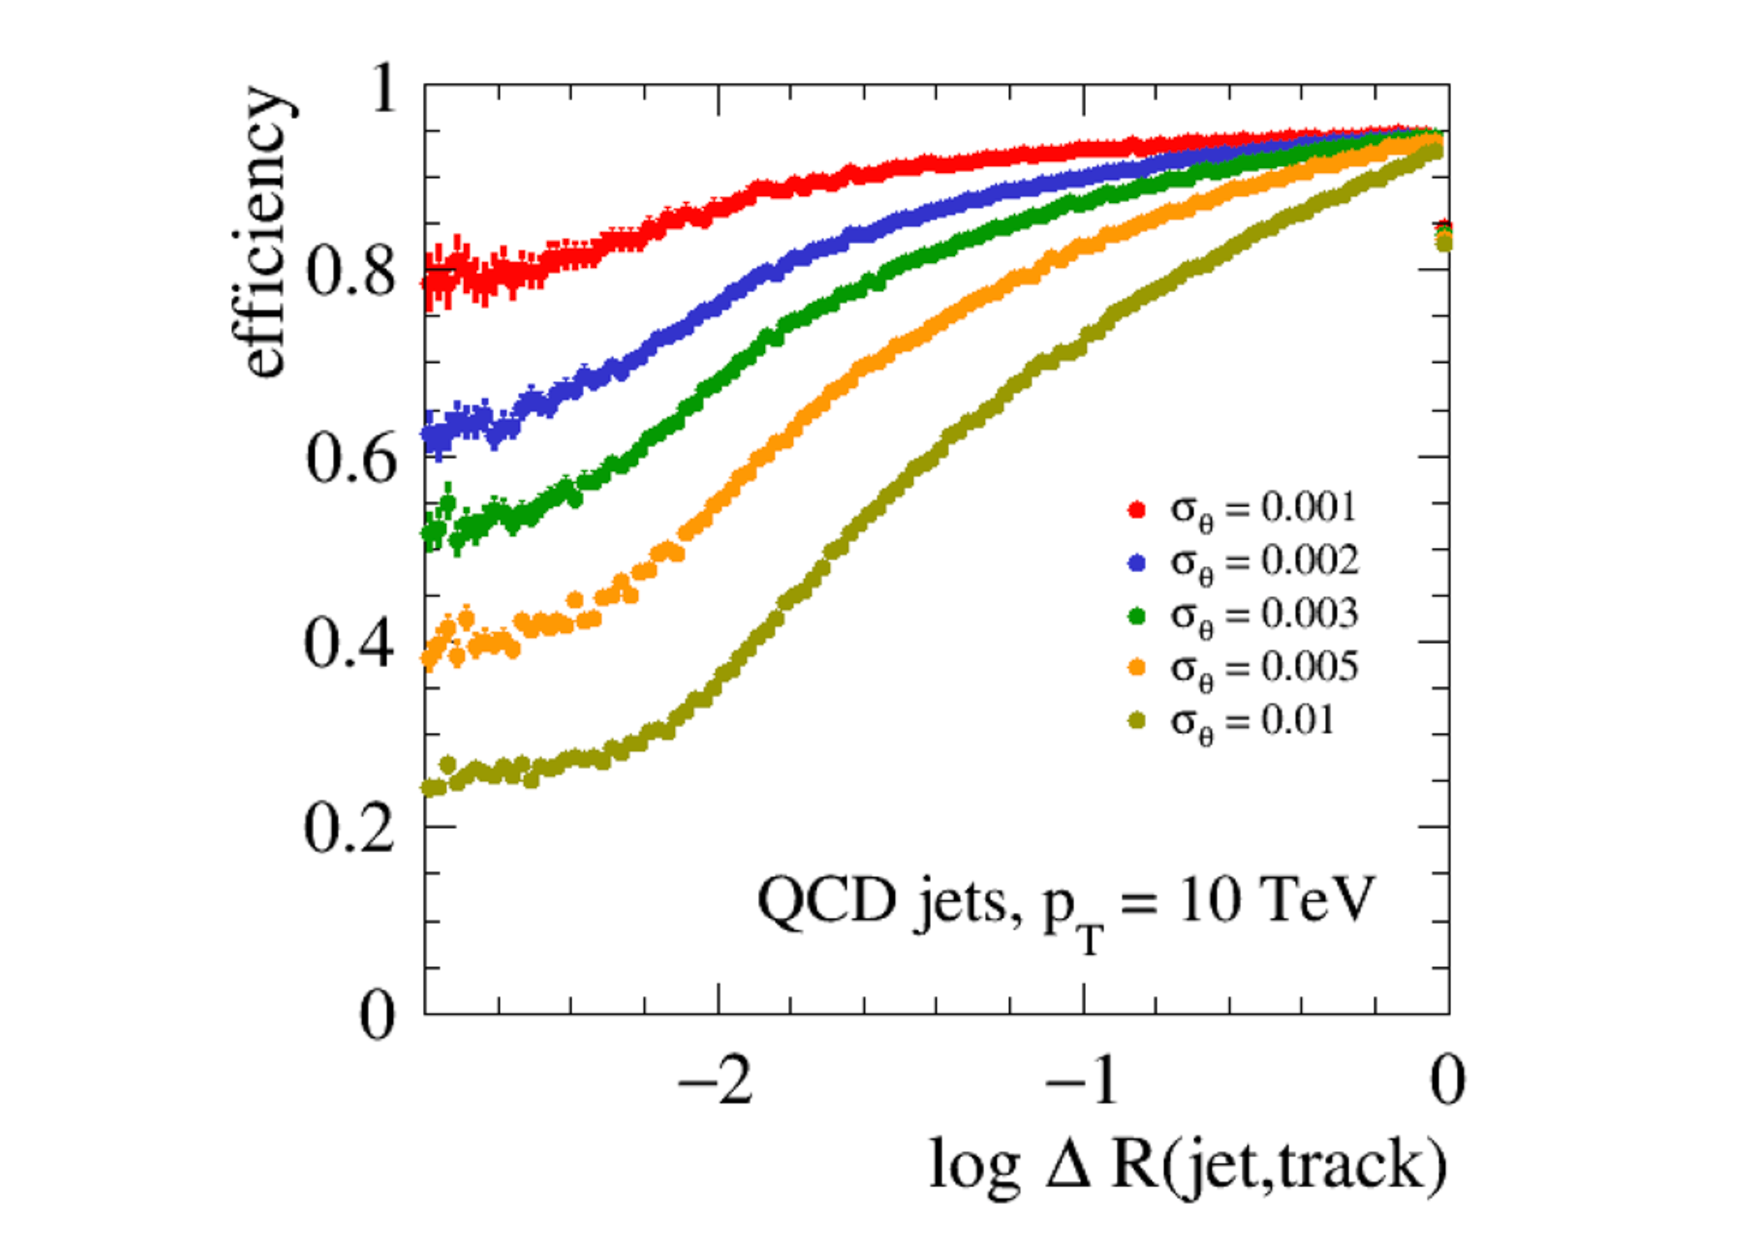
\includegraphics[width=0.56\columnwidth]{Fig/dtf.pdf}
  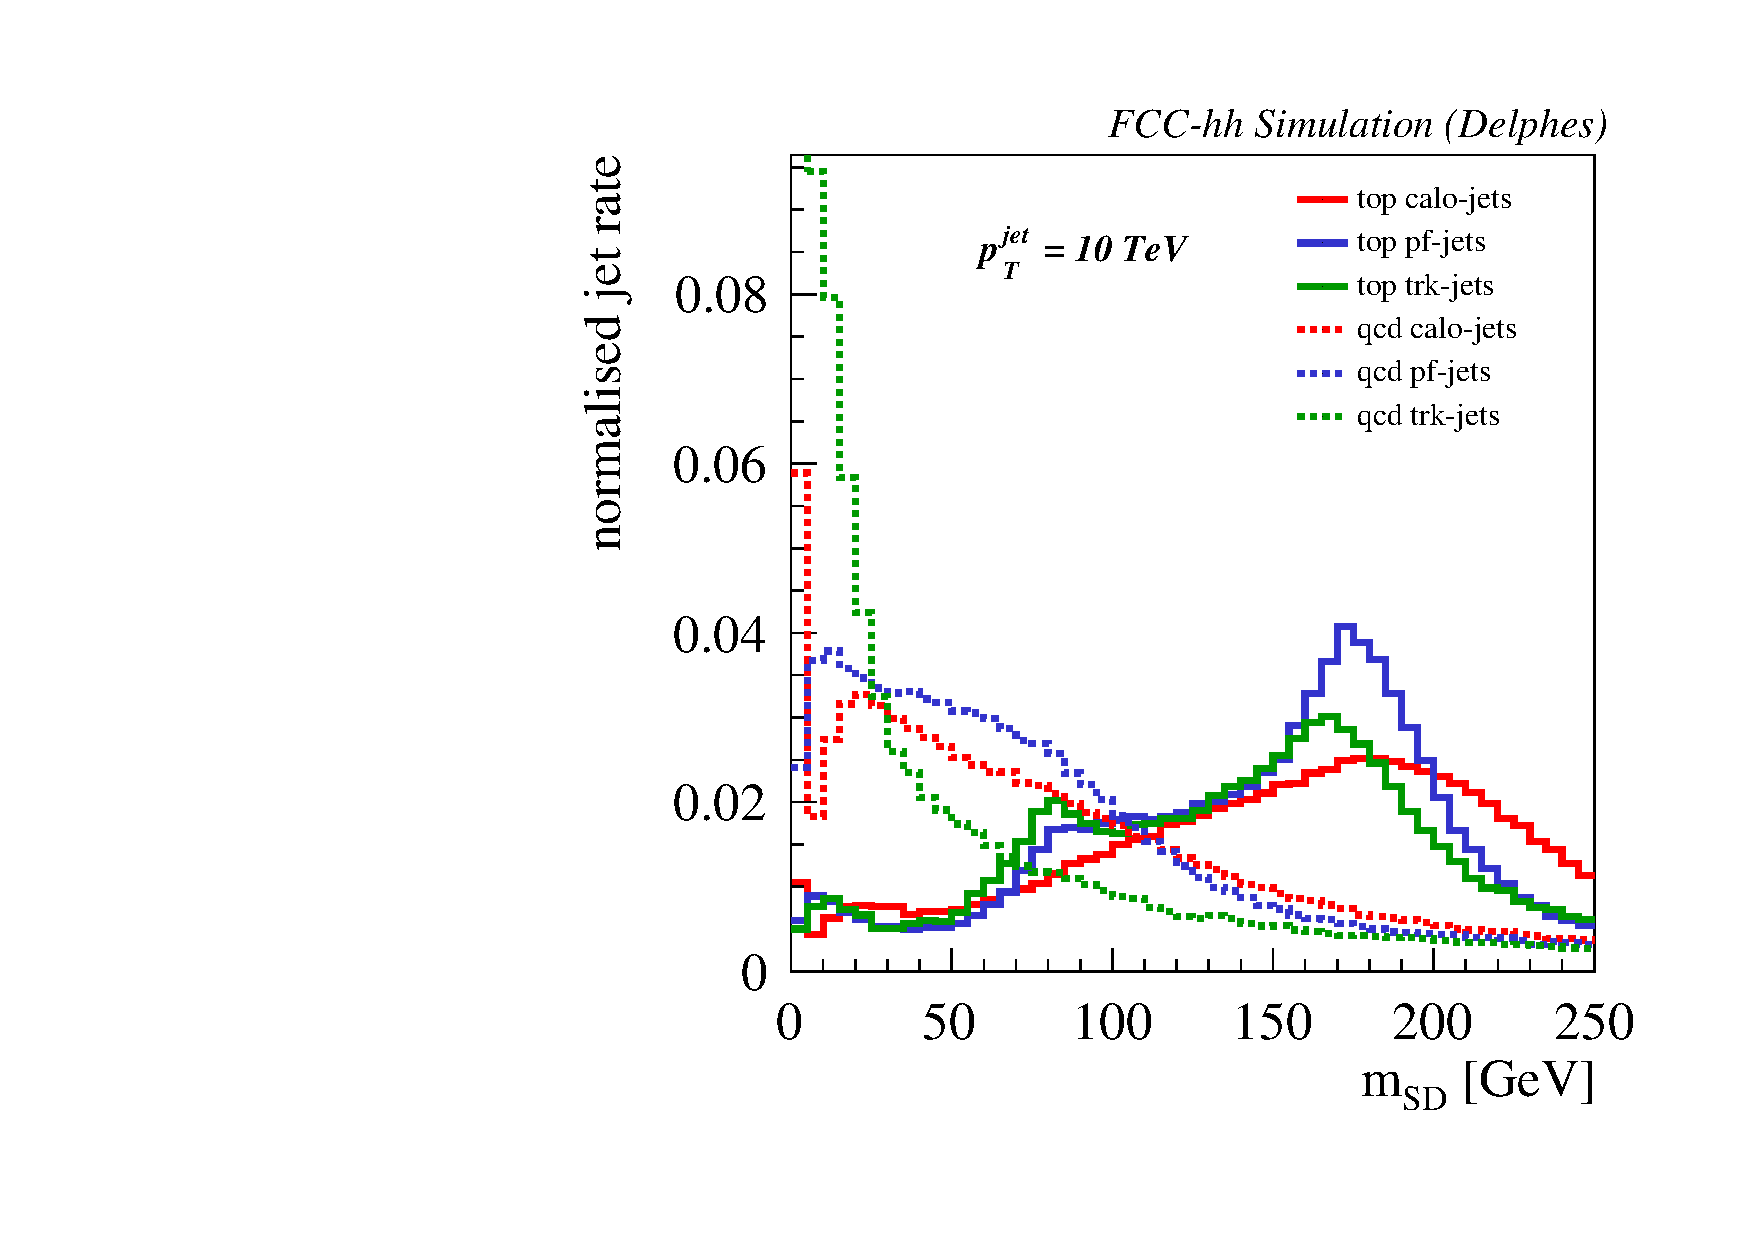
\includegraphics[width=0.42\columnwidth]{Fig/jetalgo.pdf}
  \caption{Left: Track reconstruction efficiency inside highly QCD boosted jets as function of the angular distance $\Delta R$ between the track and the center of the jet for different assumptions on the tracker spatial resolution. Right: Reconstructed 
  "soft-dropped" jet mass of highly boosted top and QCD jets with various sets of input to the jet clustering algorithm: tracks only, calorimeters towers only and particle-flow candidates. }
  \label{fig:substructure}
\end{figure}

Muons are also reconstructed using tracking. However, an additional stand-alone muon measurement is provided by the angular difference between track angle in the muon system and the radial line connection to the beam axis, giving a large improvement on the resolution at high \pt~\cite{cdr_volume3}. Assuming a 2 times better position resolution of the muon system for the FCC-hh detector, a combined muon momentum resolution of $\sigma(\pt)/\pt  \simeq 5\%$ can be achieved for momenta as high as $\pt=$~15 TeV, as opposed to $\pt=2~$TeV for the HE-LHC detector.





%%%%%%%%%%%%%%%%%%%%%%%%%%%%%%%%%%%%%%%%%%%%%%%%%%%%%
\subsubsection{Calorimetry and Particle-Flow}
\label{appsub:calorimetry}

After propagating within the magnetic field, long-lived particles reach the electromagnetic (ECAL) and hadronic (HCAL) calorimeters. Since these are modeled in \delphes{}~by two-dimensional grids of variable spacing, the calorimeter deposits natively include finite angular resolution effects. Separate grids for ECAL and HCAL have been designed for both the FCC-hh and the HE-LHC detectors in order to accurately model the angular resolution on reconstructed jets. The FCC-hh detector features an improved angular resolution by a factor 2 in the ECAL and a factor 4 in the HCAL compared to the HE-LHC detector. The energy resolution of the calorimeters is assumed to be the same for both detectors and the calorimeter parameters are summarised in Table~\ref{tab:cal_param}.

In \delphes{}~the information provided by the tracker and calorimeters is combined within the particle-flow algorithm for an optimal event reconstruction. If the momentum resolution of the tracking system is better than the energy resolution of calorimeters (typically for momenta below some threshold) the charged particles momenta are measured mainly through tracking. Vice-versa at high energy, calorimeters provide a better momentum measurement. The particle-flow algorithm exploits this complementarity to provide the best possible single charged particle measurement --- the \emph{particle-flow tracks}. These contain electron, muons and charged hadrons. Jet collections are then formed using several different input objects such as tracks (\emph{Track-jets}), calorimeter (\emph{Calo-jets}) and particle-flow candidates (\emph{PF-jets}). The Delphes framework integrates the FastJet package~\cite{Cacciari:2011ma}, allowing for jet reconstruction with the most popular jet clustering algorithms. In the present study the anti-$k_T$ algorithm~\cite{Cacciari:2008gp} is used with several jet clustering R parameters ($R=0.2, 0.4, 0.8, 1.5$).

Common jet shape observables used for jet substructure analysis such as N-subjettiness~\cite{Thaler:2010tr} and the soft-dropped mass~\cite{Larkoski:2014wba} are computed on-the-fly and stored in the output jet collections. As an illustration, the reconstructed soft-dropped mass in the FCC-hh detector for top and QCD jets with $\pt=10$~TeV and cone size $R=0.2$ is shown in Figure~\ref{fig:substructure}(right). Thanks to the superior tracker segmentation, we find \emph{Track-jets} to perform better in terms of QCD background rejection despite the slightly worse jet mass resolution.

\begin {table}[htb!]
\begin{center}
\begin{tabular}{l||c|c}
& FCC-hh & HE-LHC  \\
  \hline
  \hline
$\sigma(E)/E $ (ECAL)& 10\%/$\sqrt{E} \oplus 1\%$ &  10\%/$\sqrt{E} \oplus 1\%$\\
   \hline
$\sigma(E)/E $ (HCAL)& 50\%/$\sqrt{E} \oplus 3\%$  &  50\%/$\sqrt{E} \oplus 3\%$\\
  \hline
  \hline
$\eta \times \phi$ cell size (ECAL)& $(0.01\times0.01)$ &  $(0.02\times0.02)$\\
  \hline
 $\eta \times \phi$ cell size  (HCAL)& $(0.025\times0.025)$ & $(0.1\times0.1)$
\end{tabular}
\caption{Calorimeter parameters for the FCC-hh and HE-LHC detectors in Delphes.}
\label{tab:cal_param}
\end{center}
\end{table}
%\caption{Comparison of basic detector performances for FCC-hh and HE-LHC.}

%%%%%%%%%%%%%%%%%%%%%%%%%%%%%%%%%%%%%%%%%%%%%%%%%%%%%
\subsubsection{Object identification efficiencies}
\label{appsub:objid}

Trigger, reconstruction and identification efficiencies are parametrised as function of the particle momentum in~\delphes{}. Given that these parameterisations depend on the detailed knowledge of the detector, we simply use a global parameterisation for each object.

For electron and muons, the isolation around a cone is computed as the sum of over the full list of \emph{particle-flow candidates} within a cone $R$ excluding the particle under consideration. No selection on the isolation variable is applied during \delphes\ processing since the optimal selection working point is analysis and object dependent. Electrons and muons originating from heavy resonances are highly boosted and populate the central rapidity region of the detector. For the purpose of this study flat reconstruction identification efficiencies are assumed (see Table~\ref{tab:effs}).

The identification of jets that result from $\rm{\tau}$ decays or heavy flavour quarks --- $\rm{b}$ or $\rm{c}$ quarks --- typically involves the input from tracking information, such as vertex displacement or low level detector input such as hit multiplicity~\cite{PerezCodina:2631478,PerezCodina:2635893}. Such information is not available as a default in~\delphes{}. Instead, a purely parametric approach based on Monte-Carlo generator information is used. The probability to be identified as $\rm{b}$ or $\rm{\tau}$ depends on user-defined parameterizations(see Table~\ref{tab:effs}). The behaviour of vanilla heavy flavour tagging algorithms in regimes of extreme boosts is yet unknown. We make the conservative assumption of vanishing efficiency as a function of the transverse momentum for both $\rm{b}$ and $\rm{\tau}$-jets, as shown in Table~\ref{tab:effs}. This choice is motivated by the fact that decay products originating from highly boosted $\rm{b}$ and $\rm{\tau}$ decays will be extremely collimated and highly displaced, making their reconstruction difficult. 

\begin {table}[htb!]
\begin{center}
\begin{tabular}{ l | c | c | c | c | c }
  & electrons & muons & photons & b-jets & $\tau$-jets\\
  \hline
  \hline
FCC-hh & 99\% & 95\% & 95\%  & (1 - \pt~[TeV]/15)$\cdot$85\% & (1 - \pt~[TeV]/30)$\cdot$60\% \\
HE-LHC & 95\% & 95\% & 95\% & (1 - \pt~[TeV]/5)$\cdot$75\% & (1 - \pt~[TeV]/5)$\cdot$60\%  \\
\end{tabular}
\caption{Global reconstruction efficiency of high \pt\ central objects for the HE-LHC and FCC-hh detectors in Delphes.}
\label{tab:effs}
\end{center}
\end{table}

A mis-tagging efficiency, that is, the probability that a particle other than $\rm{b}$ or $\rm{\tau}$ be wrongly identified as a $\rm{b}$ or a $\rm{\tau}$ has been included in the simulation and assumes a similar falling behaviour as a function of the jet momentum. For the b-tagging, the mistag efficiency are parameterised separately for light-jets (uds-quarks) and c-jets. For the $\tau-$tagging we consider only mis-identification from QCD jets. Table~\ref{tab:mistag} summarises the main values for the mis-tagging efficiency.

\begin {table}[htb!]
\begin{center}
\begin{tabular}{ l | c | c | c }
  & light (b-tag) & charm (b-tag) & QCD ($\tau$-tag)\\
  \hline
  \hline
FCC-hh & (1 - \pt~[TeV]/15)$\cdot$1\% & (1 - \pt~[TeV]/15)$\cdot$5\% & (8/9 - \pt~[TeV]/30)$\cdot$1\% \\
HE-LHC & (1 - \pt~[TeV]/5)$\cdot$1\%  & (1 - \pt~[TeV]/5)$\cdot$10\% & (1 - \pt~[TeV]/5)$\cdot$1\%  \\
\end{tabular}
\caption{Mis-identification efficiency of high \pt\ central heavy flavour jets for the HE-LHC and FCC detectors in Delphes.}
\label{tab:mistag}
\end{center}
\end{table}



%%%%%%%%%%%%%%%%%%%%%%%%%%%%%%%%%%%%%%%%%%%%%%%%%%%%%
%%%%%%%%%%%%%%%%%%%%%%%%%%%%%%%%%%%%%%%%%%%%%%%%%%%%%
\subsection{Treatment of the Monte-Carlo samples}
\label{subsec:mctreat}
The modelling of the backgrounds in the high tagging regimes is a challenging task. The requirement of $b$ tagging in some MC samples can drastically reduce the available statistics. This shortage of events that pass the $b$-tagging cut in the signal regime, in conjunction with the large cross section of some of the backgrounds can lead to very spiky templates. To overcome this problem the tag rate function (TRF) method is used. By using the TRF method, no event is cut based on its $b$-tagging count, but instead all the events are weighted. This weight can be interpreted as the probability of the given event to contain the desired number of $b$ jets. To achieve this, the tagging efficiency (a function of $\eta$, $\pt$ and true jet flavour) was used to calculate the event weight based on the kinematics and flavour of the jets found in each event. 
Despite the fact that very large amount of Monte-Carlo statistic has been simulated in bins of $\hht$ and the usage of TRF to save events, there are still large statistical fluctuations from high weight events. In order to reduce this effect, and when large fluctuations are observed, the background spectrum is fitted. Further details on the TRF and fitting procedure are given in Appendix~\ref{sec:app:trf}.
and~\ref{sec:app:bgfit} respectively.

%%%%%%%%%%%%%%%%%%%%%%%%%%%%%%%%%%%%%%%%%%%%%%%%%%%%%
\subsection{Statistical analysis}
Hypothesis testing is performed using a modified frequentist method based on a profile likelihood that takes into account the systematic uncertainties as nuisance parameters that are fitted to the expected Monte-Carlo. The full shape information is used, which help from the sidebands to reduce the effect of systematics uncertainties in the signal region. The test statistic $q_\mu$ is defined as the profile log-likelihood ratio: $q_\mu = -2\ln({\cal L}(\mu,\hat{\hat{\theta}}_\mu)/{\cal L}(\hat{\mu},\hat{\theta}))$, where $\hat{\mu}$ and $\hat{\theta}$ are the values of the parameters that maximise the likelihood function (with the constraint $0\leq \hat{\mu} \leq \mu$), and $\hat{\hat{\theta}}_\mu$ are the values of the nuisance parameters that maximise the likelihood function for a given value of $\mu$. In the absence of any significant deviation from the background expectation, $q_\mu$ is used in the CL$_\text{s}$ method~\cite{Junk:1999kv,Read:2002hq} to set an upper limit on the signal production cross-section times branching ratio at the 95\% CL. For a given signal scenario, values of the production cross-section (parameterised by $\mu$) yielding CL$_\text{s} < 0.05$, where CL$_\text{s}$ is computed using the asymptotic approximation~\cite{Cowan:2010js}, are excluded at 95\% CL. For a $5\sigma$ discovery, the quantity 1-CL$_\text{b}$ must be smaller than $2.87 \cdot 10^{-7}$~\cite{Junk:1999kv} and is also computed using the asymptotic approximation.



%%%%%%%%%%%%%%%%%%%%%%%%%%%%%%%%%%%%%%%%%%%%%%%%%%%%%
\section{Di-lepton channels}
\label{sec:lep}

The decay products of heavy resonances are in the multi-TeV regime and the capability to reconstruct their momentum imposes stringent requirement on the detector design. In particular, reconstructing the track curvature of multi-TeV muons requires excellent position resolution and a large lever arm. In this section, the expected sensitivity is presented for a \Zpll\ (where $\ell=e,\mu$) and \Zptata\ separately.

%%%%%%%%%%%%%%%%%%%%%%%%%%%%%%%%%%%%%%%%%%%%%%%%%%%%%
\subsection{The \texorpdfstring{\ee}{ee} and \texorpdfstring{\mumu}{mumu} final states}
\label{sec:lepee}

Events are required to contain two isolated opposite sign leptons with $\pt > 1$\,TeV, $|\eta|$<4 and an invariant mass \mll\ > 2.5\,TeV.
Figure~\ref{figure:leptonicresonances:ll} left shows the invariant mass for a 30\,TeV \ZpSSM\ signal for the $\mu\mu$ channel. The di-electron invariant mass spectrum is not shown, but as expected from the calorimeter constant term that dominates the resolution at high \pt, the mass resolution is better for the $ee$ channel.
The di-lepton invariant mass spectrum is used as the discriminant and a 50\% normalisation uncertainty on the background normalisation is assumed.
Figure~\ref{figure:leptonicresonances:ll} (bottom left) shows the 95\% CL exclusion limit obtained with 30\,ab$^{-1}$ of data combining ee and $\mu\mu$ channels. Figure~\ref{figure:leptonicresonances:ll} (bottom right) shows the integrated luminosity required to reach a $5\sigma$ discovery as a function of the mass of the heavy resonance. The \Zpee\ and \Zpmumu\ channel display very similar performance due to the low background rates. We conclude therefore that the reference detector design features near to optimal performance for searches involving high \pt\ muon final states. Combining $ee$ and $\mu\mu$ channels, masses up to 42\,TeV can be excluded or discovered.

\begin{figure}[!htb]
  \centering
%  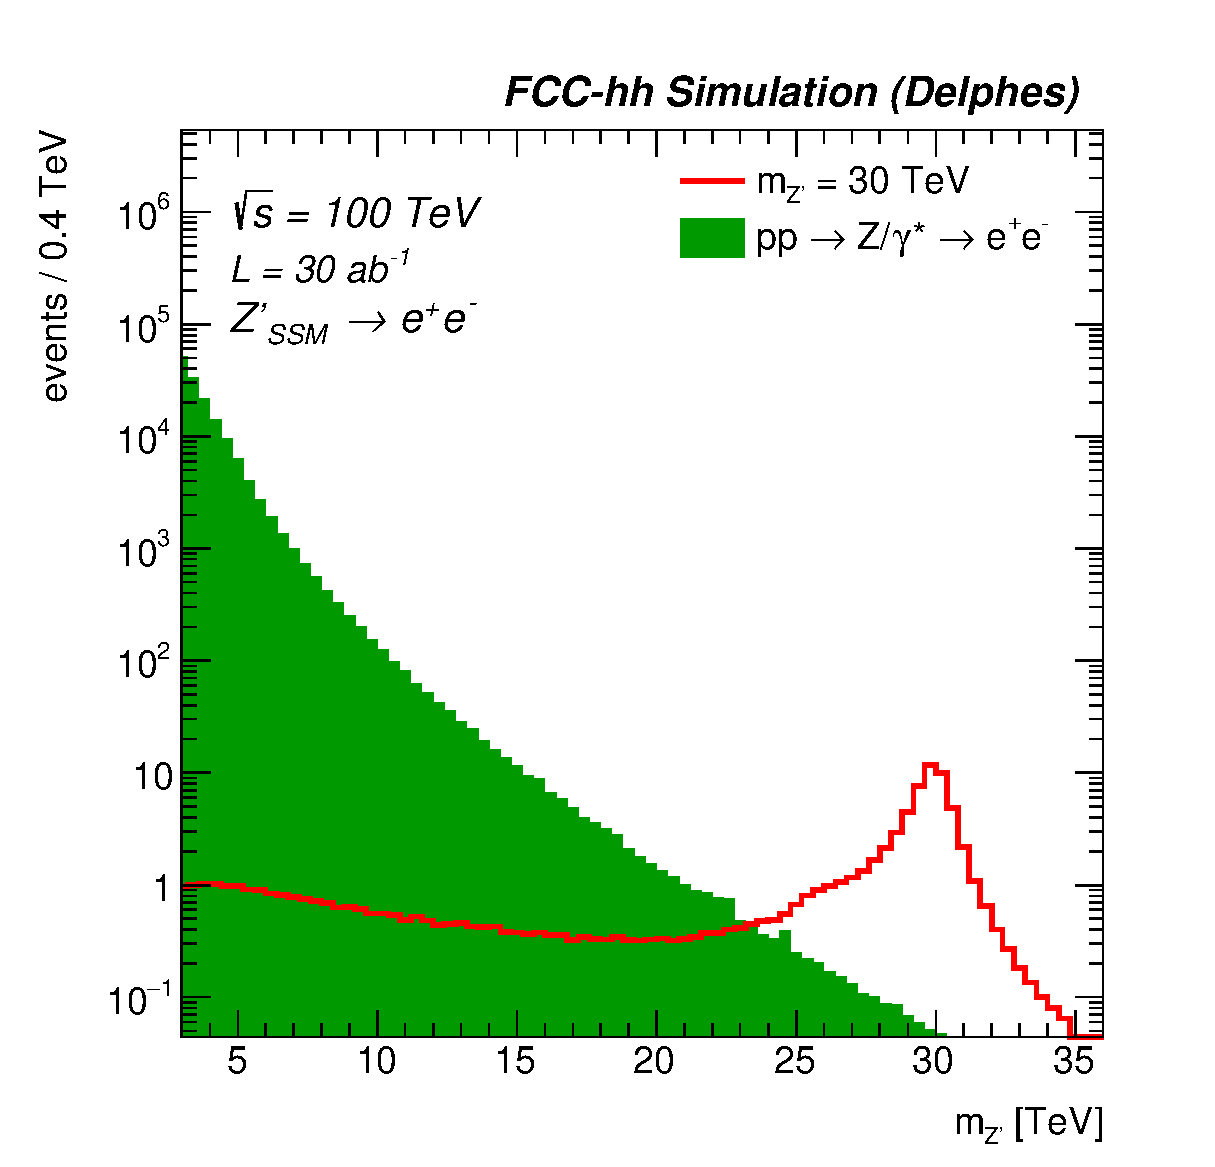
\includegraphics[width=0.35\columnwidth]{Fig/mzp_sel0_nostack_log_ee.eps}
  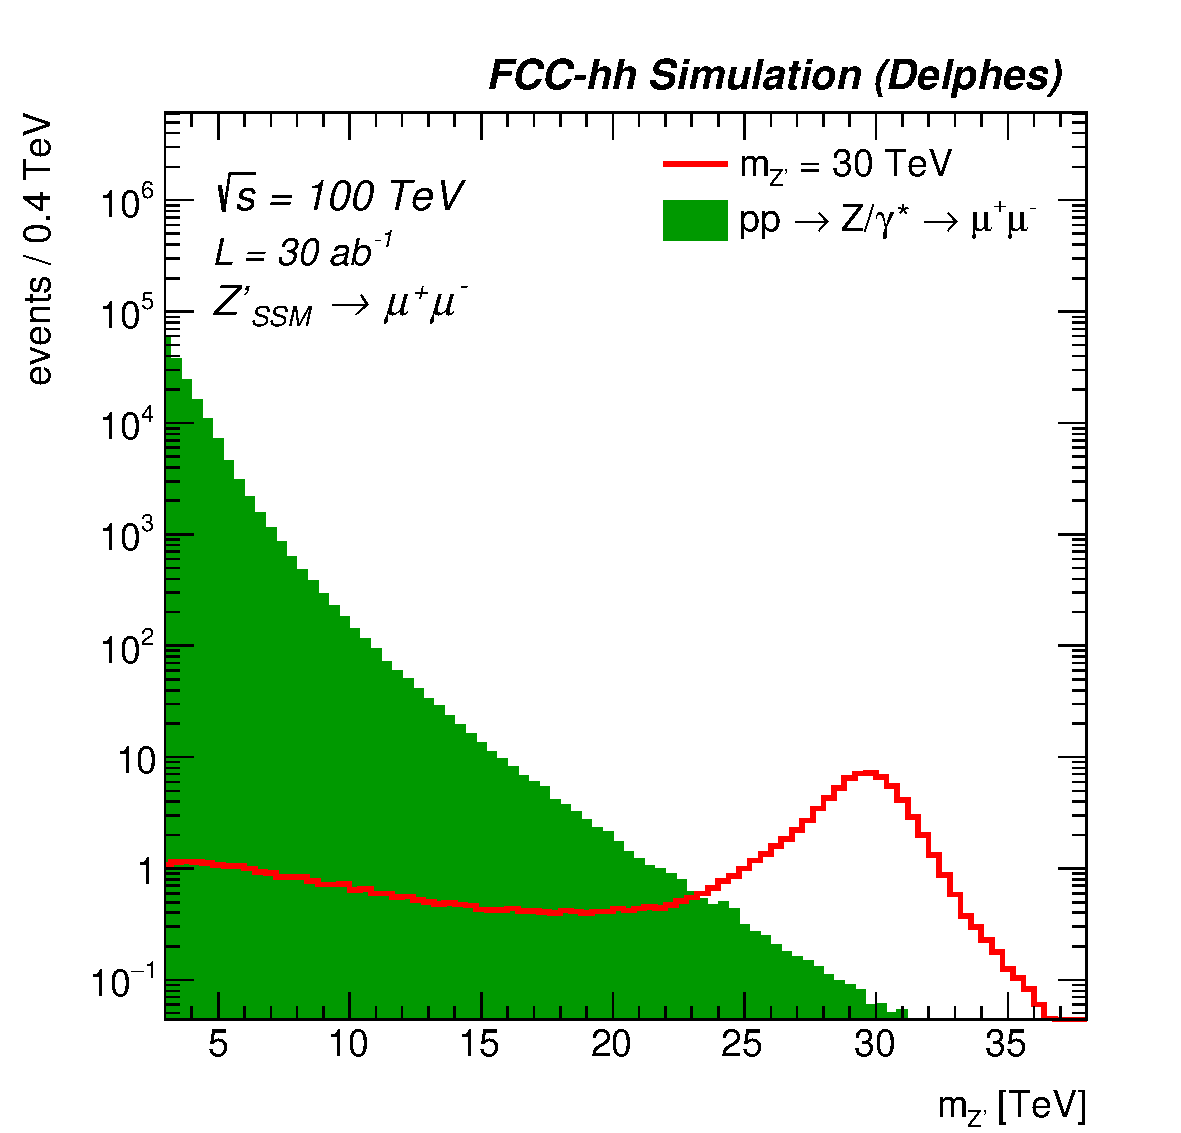
\includegraphics[width=0.32\columnwidth]{Fig/mzp_sel0_nostack_log_mm-eps-converted-to.pdf}
  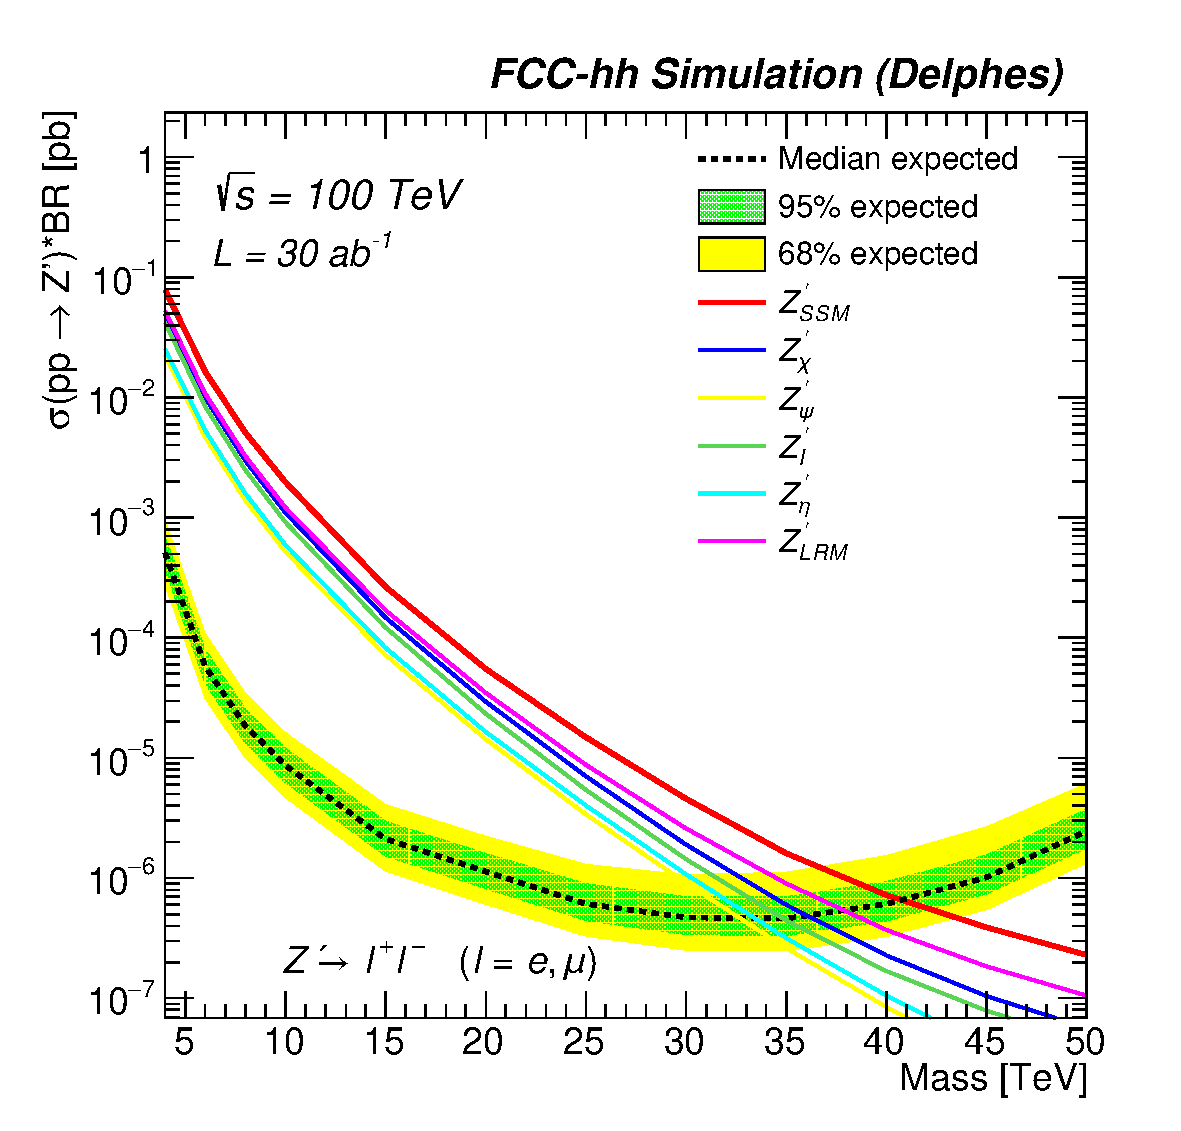
\includegraphics[width=0.32\columnwidth]{Fig/lim_Zprime_ll_fcc_v02_allxs-eps-converted-to.pdf}
  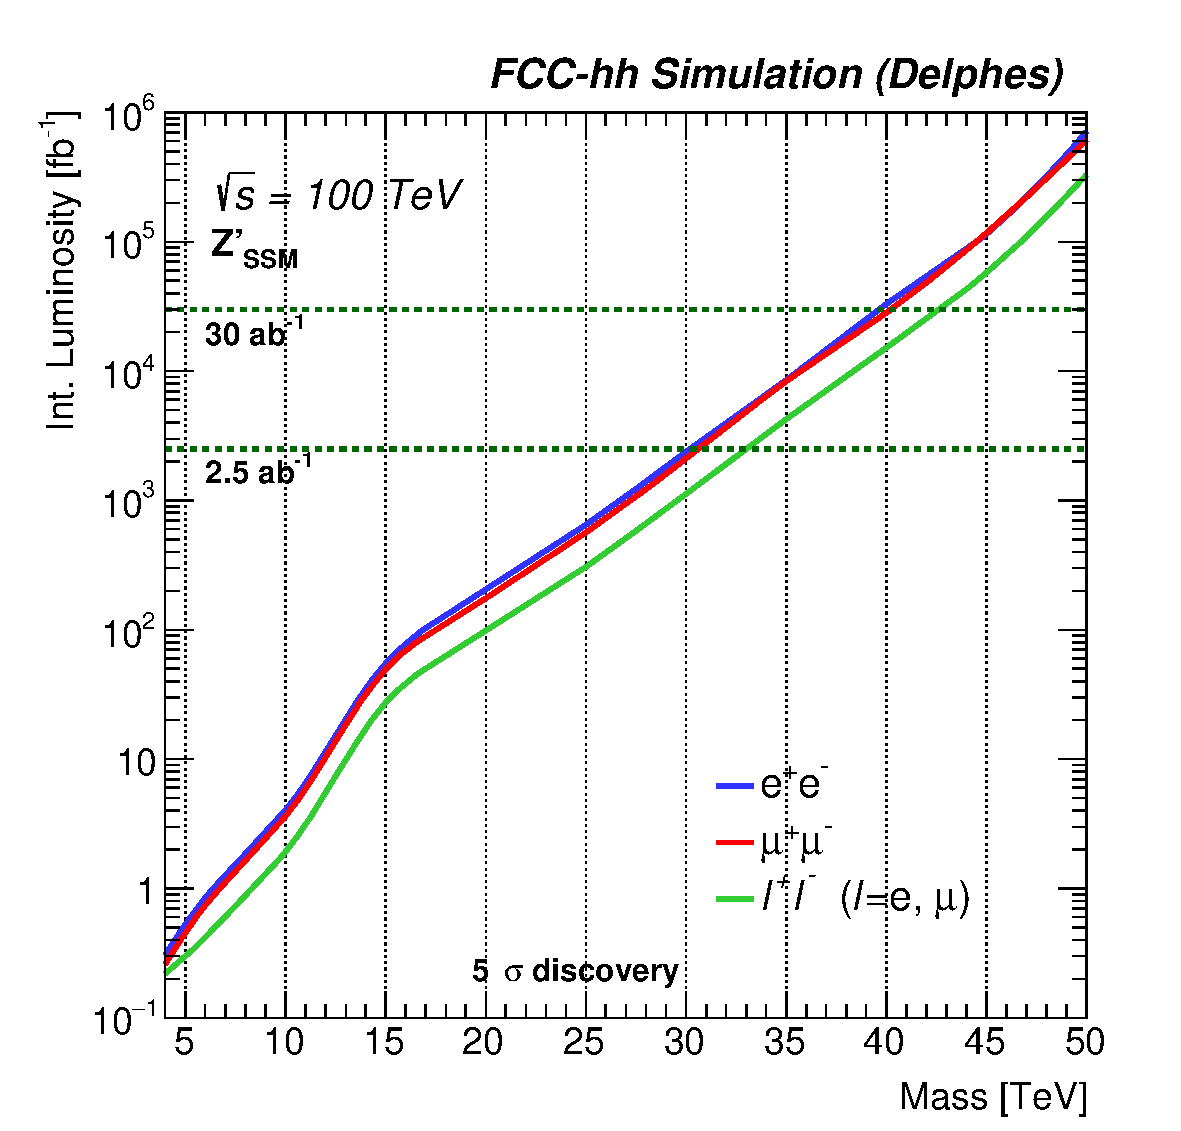
\includegraphics[width=0.32\columnwidth]{Fig/DiscoveryPotential_ll_comb_rootStyle-eps-converted-to.pdf}
  \caption{Left: Invariant mass for a 30\,TeV signal after full event selection for the $\mu\mu$ channel. Middle: 95\% CL limit versus mass for the combined di-lepton ($ee$, $\mu\mu$) channel. Right: integrated luminosity versus mass for a $5\sigma$ discovery comparing ee, $\mu\mu$ and combined channels.}
  \label{figure:leptonicresonances:ll}
\end{figure}



%%%%%%%%%%%%%%%%%%%%%%%%%%%%%%%%%%%%%%%%%%%%%%%%%%%%%
\subsection{The \texorpdfstring{\tautau}{tautau} final state}
\label{sec:leptautau}

At current LHC~\cite{Khachatryan:2016qkc}, the most sensitive channel to search for high mass di-$\tau$ resonances is when both $\tau$ leptons decays hadronically, and this is the focus of the analysis presented in this section. The event selection requires two jets with $p_{T} > 0.5$\,TeV and $|\eta|<2.5$, both identified as $\tau$'s. To ensure no overlap between the $\ell=e,\mu$ and $\tau$ final states, jets containing an electron or a muon with $\pt > 100$\,GeV are vetoed. Finally, requirements of $\Delta \phi(\tau_1, \tau_2)> 2$ and $2.5<\Delta R(\tau_1, \tau_2)<4$ are applied to suppress multi-jet background. Furthermore, mass dependent cuts are applied to maximise the signal significance and are summarised in Table~\ref{tab:leptonicresonances:tautau}. Several proxies for the true resonance mass have been tested, such as the invariant mass of the two $\tau$'s, with and without correction for the missing energy, but the transverse mass~\footnote{the transverse mass is defined as $m_{T}  =  \sqrt{2\ptZp*\met*(1-cos\Delta\phi(\Zp,\met))} $} provided the best sensitivity and is therefore used to estimate the sensitivity.
Figure~\ref{figure:leptonicresonances:tautau} shows the di-$\tau$ transverse mass (left) for a 10\,TeV \ZpSSM, the 95\% CL exclusion limits for 30\,ab$^{-1}$ of data (middle) and the required integrated luminosity versus mass of the resonance to reach a $5\sigma$ discovery (right). Heavy resonance decaying to $\tau$ leptons reconstructed in the hadronic decay mode are more challenging given the overwhelming multi-jet background, but masses up to 18\,TeV could be probed. The tau-tagging efficiencies considered in this analysis are assumed to be pessimistic, but only a study made in full simulation could provide realistic numbers, and should be performed in a later stage of the study.

\begin{table}[htb!]
   \centering
\begin{tabular}{c|c|c|c}
   $\Zp$ mass [TeV] &  $\Delta \phi(\tau_1, \tau_2)$&  $\Delta R(\tau_1, \tau_2)$ & $\met$\\
  \hline
  \hline
  $4-8$ & > 2.4 & > 2.5 and < 3.5 & > 400 GeV\\
  $10$ & > 2.4 & > 2.7 and < 4 & > 300 GeV\\
  $12-14$ & > 2.6 & > 2.7 and < 4 & > 300 GeV\\
  $16-18$ & > 2.7 & > 2.7 and < 4 & > 300 GeV\\
  $>18$ & > 2.8 & > 3 and < 4 & > 300 GeV\\
  \end{tabular}
  \caption{List of mass dependent cuts optimised to maximise the sensitivity for the \Zptata\ search.}
  \label{tab:leptonicresonances:tautau}
\end{table}


\begin{figure}[htb!]
  \centering
  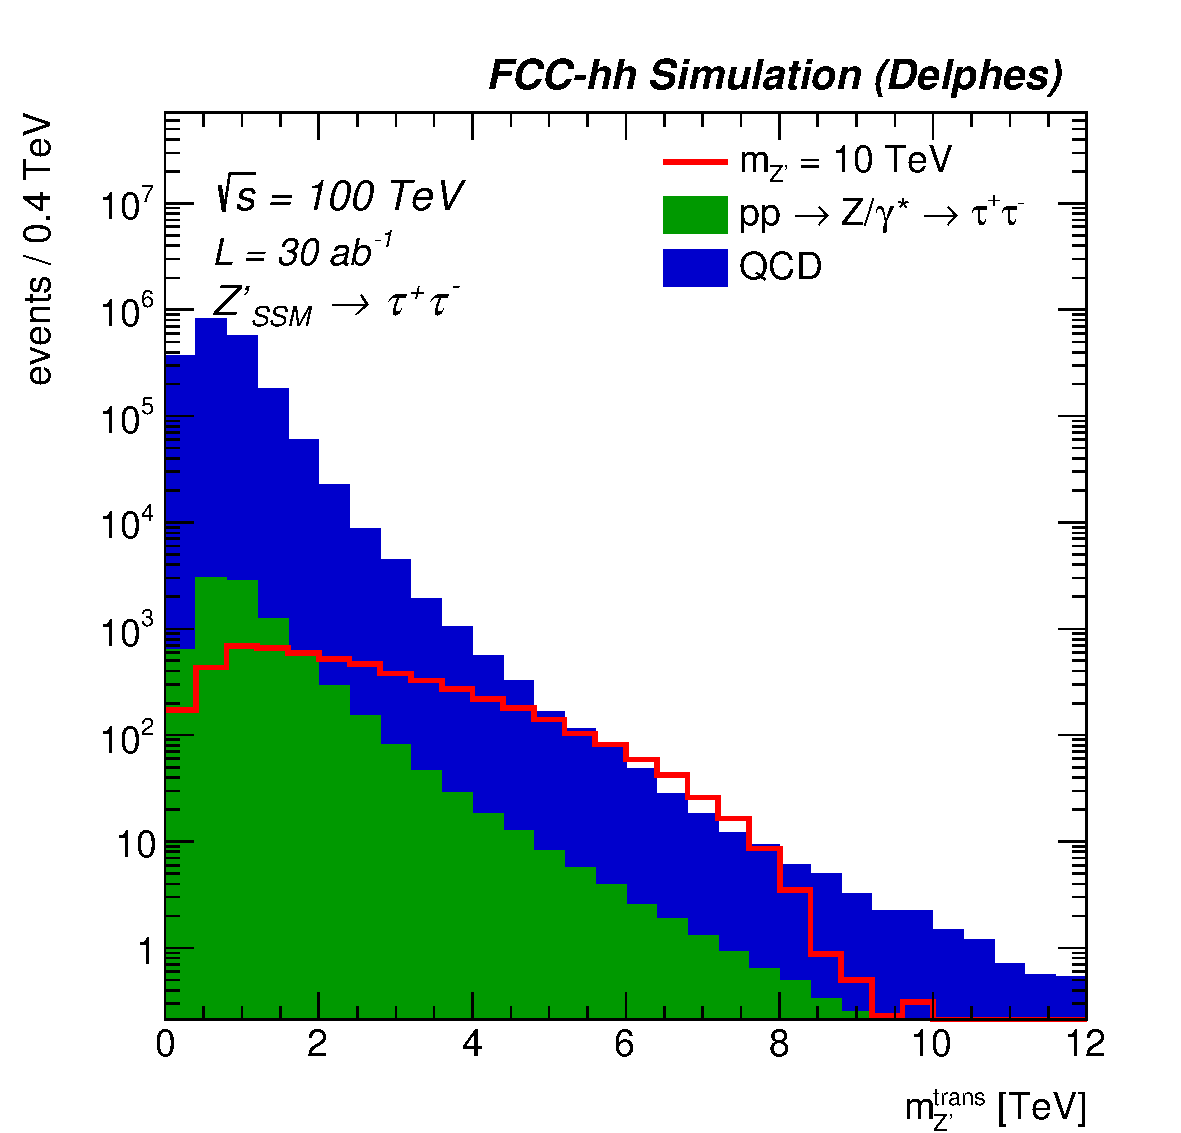
\includegraphics[width=0.32\columnwidth]{Fig/mt_finalsel_nostack_log-eps-converted-to.pdf}
  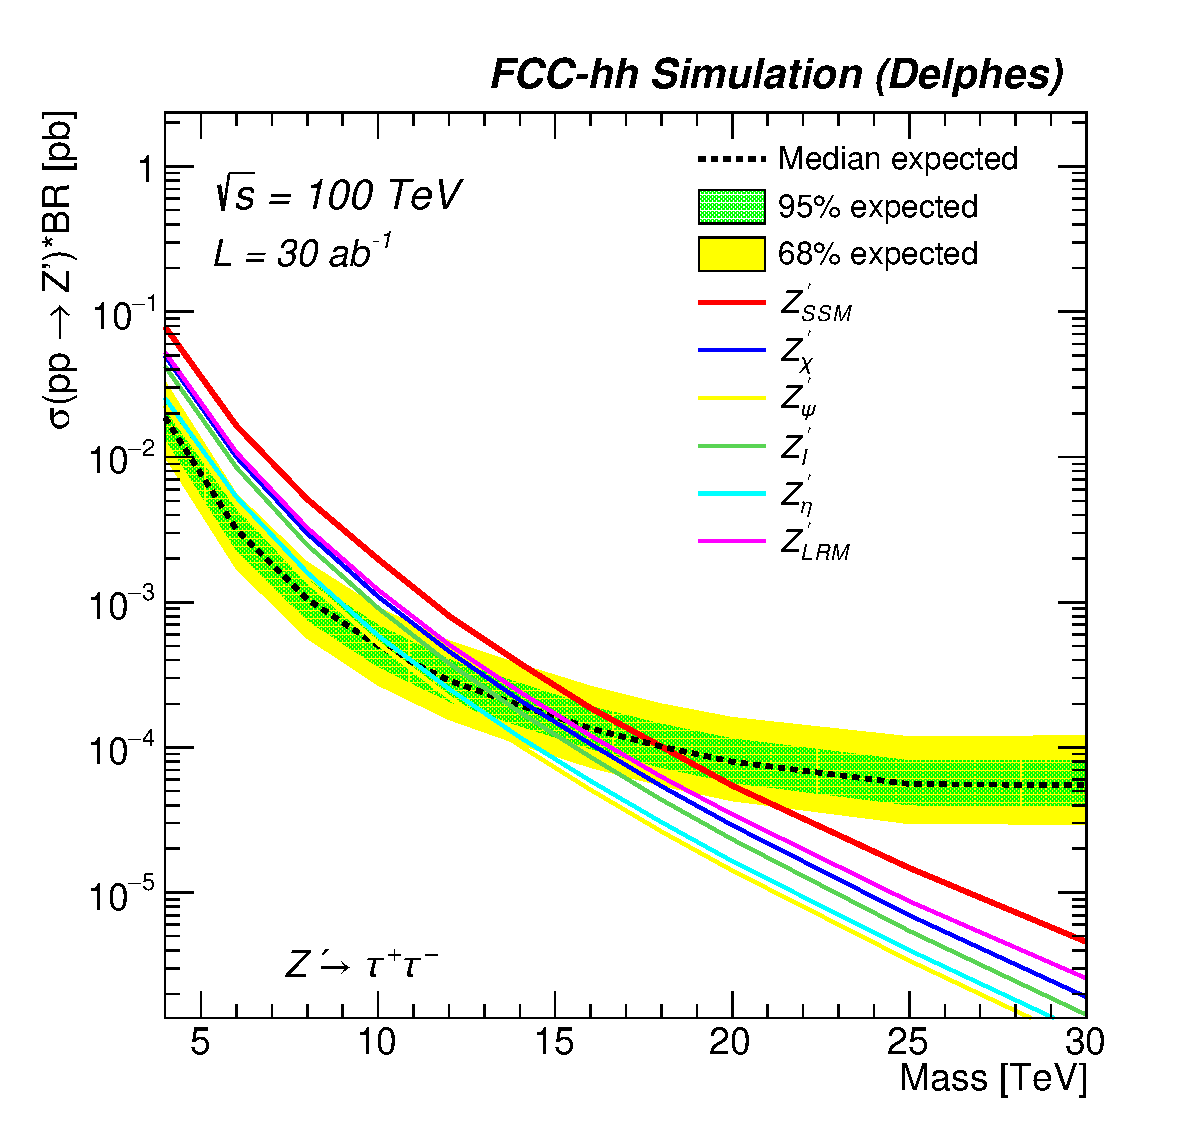
\includegraphics[width=0.32\columnwidth]{Fig/lim_Zprime_tautau_fcc_v02_allxs_fullmt-eps-converted-to.pdf}
 % 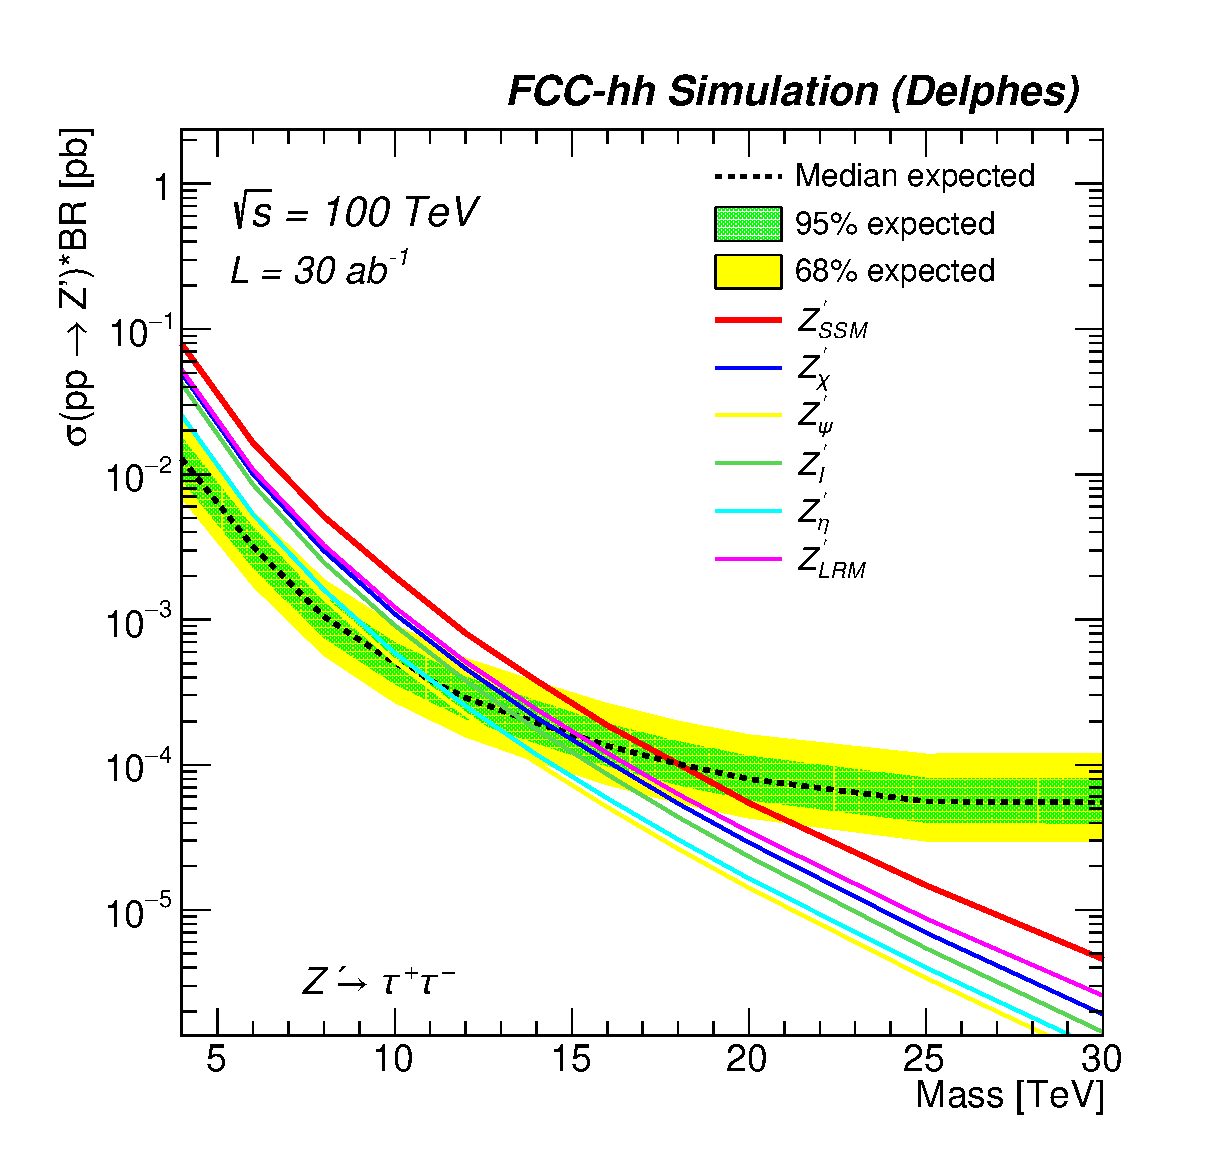
\includegraphics[width=0.32\columnwidth]{Fig/lim_Zprime_tautau_fcc_v02_allxs_mt_4TeVmzp.eps}
  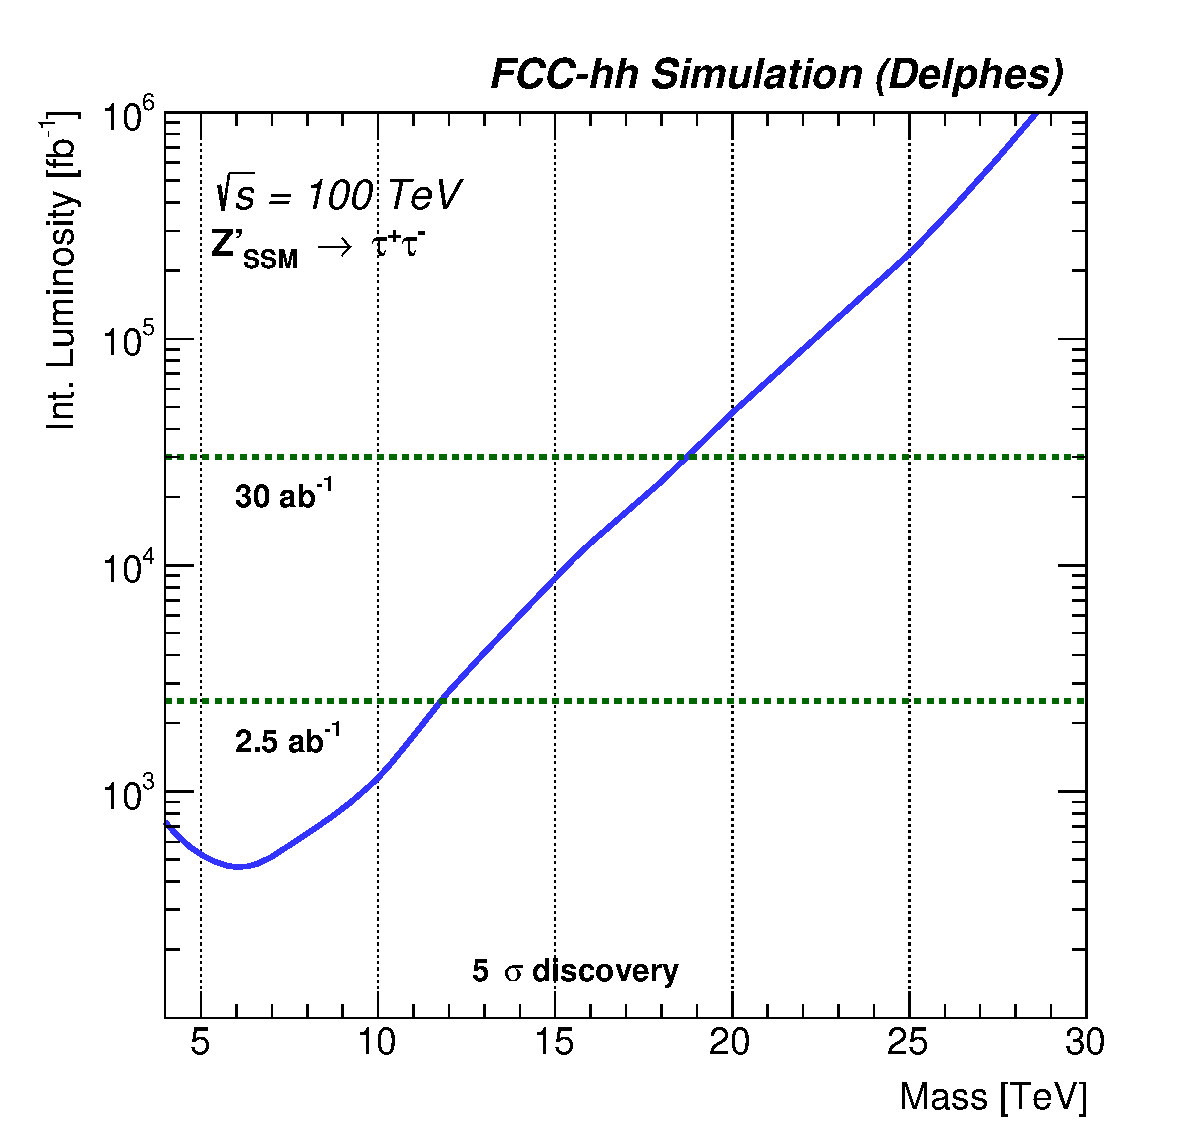
\includegraphics[width=0.32\columnwidth]{Fig/DiscoveryPotential_tautau_rootStyle_fullmt-eps-converted-to.pdf}
%  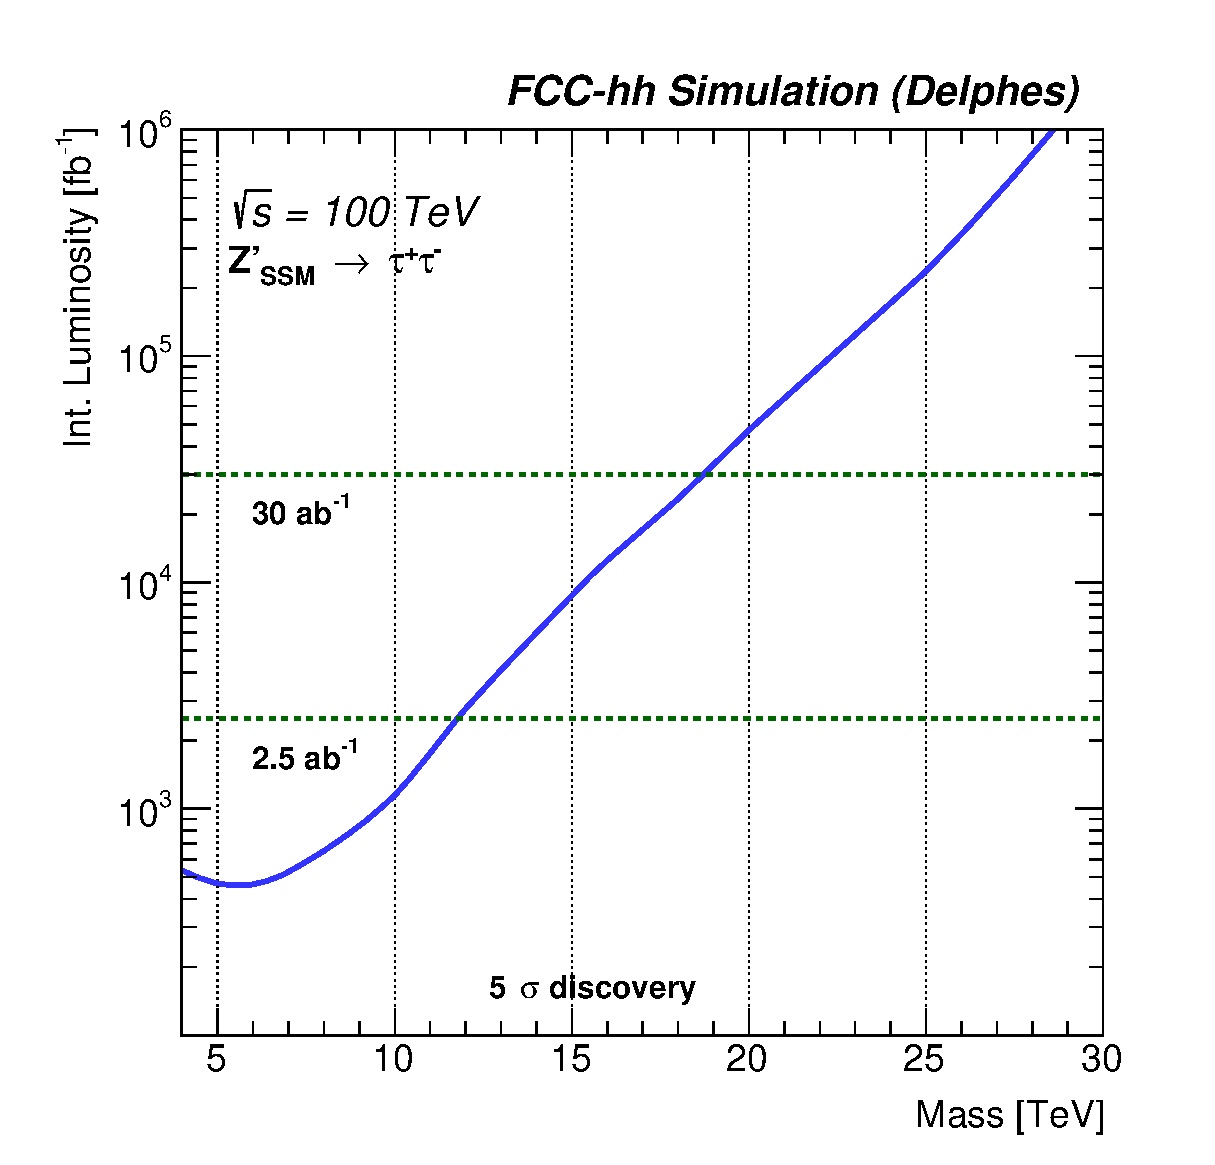
\includegraphics[width=0.32\columnwidth]{Fig/DiscoveryPotential_tautau_rootStyle_mt_4TeVmzp.eps}
  \caption{Left: Di-$\tau$ transverse mass for a 10\,TeV signal after full event selection. Middle: 95\% CL limit versus mass. Right: integrated luminosity versus mass for a $5\sigma$ discovery.}
  \label{figure:leptonicresonances:tautau}
\end{figure}


%%%%%%%%%%%%%%%%%%%%%%%%%%%%%%%%%%%%%%%%%%%%%%%%%%%%%
\section{Hadronic final states}
\label{sec:hadronic}

Heavy resonances decaying hadronically also imposes stringent requirement on the detector design. For instance,  precise jet energy resolution requires full longitudinal shower containment and highly boosted top quarks and $W$ bosons decay into highly collimated jets that need to  be disentangled from standard QCD jets by studying their substructure. High discrimination power and sensitivity for these searches at such extreme energies, requires excellent granularity both in the tracking detectors and calorimeters.

%%%%%%%%%%%%%%%%%%%%%%%%%%%%%%%%%%%%%%%%%%%%%%%%%%%%%
\subsection{Multi-Variate object tagging}
\label{subsec:mvatagger}

% from physics paper
An important ingredient of the hadronic searches is the identification of heavy boosted top quarks and $W$ bosons. Two object level taggers using Boosted Decision Trees (BDT) were developed to discriminate $W$ and top jets against the light jet flavours treated as background.
Top and $W$ taggers were optimised using jets with a transverse boost of $\pt=$10 TeV. At these extreme energies, $W$ and top jets have a characteristic angular size $R=0.01-0.02$, i.e smaller than the typical electromagnetic and hadronic calorimeter cells. Following the approach described in~\cite{Larkoski:2015yqa}, we exploit the superior track angular resolution and reconstruct jets from tracks only using the anti-$k_T$ algorithm with a parameter R=0.2, but also larger values are used to increase the discrimination power of the BDT. The missing neutral energy is corrected for by rescaling the track 4-momenta by the factor $\ptSub{,trk}/\ptSub{,PF}$, where $\ptSub{,trk}$ is the track Jet \pt\ and $\ptSub{,PF}$ is the Particle-Flow (PF) Jet \pt. In what follows, we will simply refer to ``track jets'' as the jet collection that includes the aforementioned rescaling. The boosted top tagger is built from jet substructure observables: the soft-dropped jet mass~\cite{Larkoski:2014wba} (\mSD) and N-subjettiness~\cite{Thaler:2010tr} variables $\tau_{1,2,3}$ and their ratios $\tau_{2}/\tau_{1}$ ($\tau_{21}$) and $\tau_{3}/\tau_{2}$ ($\tau_{32}$). The $W$-jet tagger also uses an ``isolation-like'' variable that exploits the absence of high \pt\ final state-radiation (FSR) in the vicinity of the $W$ decay products. We call these variables $E_{F}(n,\alpha)$ and define them as:

%\begin{equation}
%E_{F}(n,\alpha) =  \frac{\sum \limits_{\frac{n-1}{5}\alpha < \Delta R(k,jet)< \frac{n}{5}\alpha} \ptSup{(k)}}{\sum \limits_{\Delta R(k,jet)< \alpha} \ptSup{(k)}}
%\end{equation}

\begin{equation}
E_{F}(n,\alpha) =  \sum \limits_{\frac{n-1}{5}\alpha < \Delta R(k,jet)< \frac{n}{5}\alpha} \ptSup{(k)} \Biggm/ \sum \limits_{\Delta R(k,jet)< \alpha} \ptSup{(k)}
\end{equation}
with $k$ running over the jet constituents and $\alpha=0.05$. We construct 5 variables $E_{F}(n,\alpha)$ with $n=[1,2,3,4,5]$ and use them as input to the BDT.
The $W$ tagging performance has significantly better performance due to the good discrimination power of the energy-flow variables. We choose the working points for the analyses presented later with a top and $W$ tagging efficiencies of $\epsilon_S^{\text{top}}=60\%$ and $\epsilon_S^{\text{W}}=90\%$ corresponding respectively to a background rejection of $\epsilon_B^{\text{top}}=\epsilon_B^{\text{W}}=90\%$. These working points corresponds to a cut at 0.15 on the BDT value for both taggers. Independent samples have been generated for the training of the BDT in such a way that there is no overlap with the events used in the analysis.  More details on the multi-Variate object tagging can be found in Appendix~\ref{sec:app:mva}.

%%%%%%%%%%%%%%%%%%%%%%%%%%%%%%%%%%%%%%%%%%%%%%%%%%%%%
\subsection{The \jj\ final state}
\label{sec:hadjj}

Jets are clustered using particle-flow candidates with the anti-$k_T$~\cite{Cacciari:2008gp} algorithm and  parameter R=0.4. We require at least two very energetic jets with $\pt$>3\,TeV and $|\eta|<3$. As di-jet events from signal will tend to be more central than for background, the rapidity difference between the two leading jets $\Delta(\eta_1, \eta_2)$ is required to be smaller than 1.5. The di-jet invariant mass for the \qjj\ signal with a mass of 40\,TeV together with the QCD contribution after the full event selection is shown on Figure~\ref{figure:hadronicresonances:jj} (left). The middle Figure shows the 95\% CL exclusion limit obtained with 30\,ab$^{-1}$ of data and the right Figure shows the integrated luminosity required to reach a $5\sigma$ discovery as a function of the Q$^*$ mass. For this very simple case of strongly coupled object we reach 95\% CL exclusion limits of 43\,TeV and 5$\sigma$ discovery reach of 40\,TeV with 30\,ab$^{-1}$ of integrated luminosity. 

\begin{figure}[!htb]
  \centering
  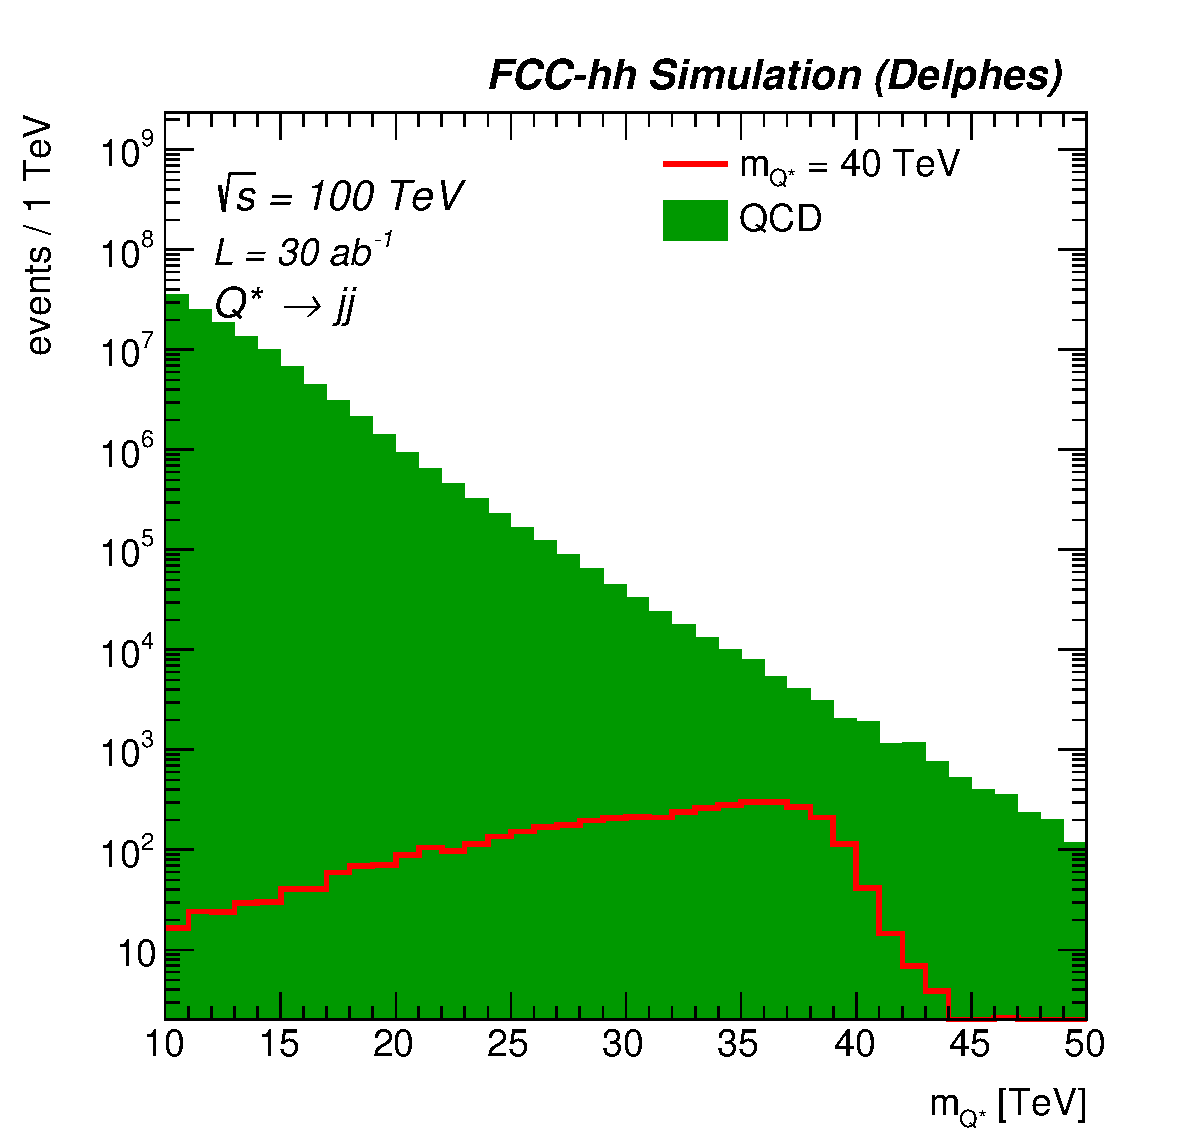
\includegraphics[width=0.32\columnwidth]{Fig/Mj1j2_pf04_sel1_nostack_log-eps-converted-to.pdf}
  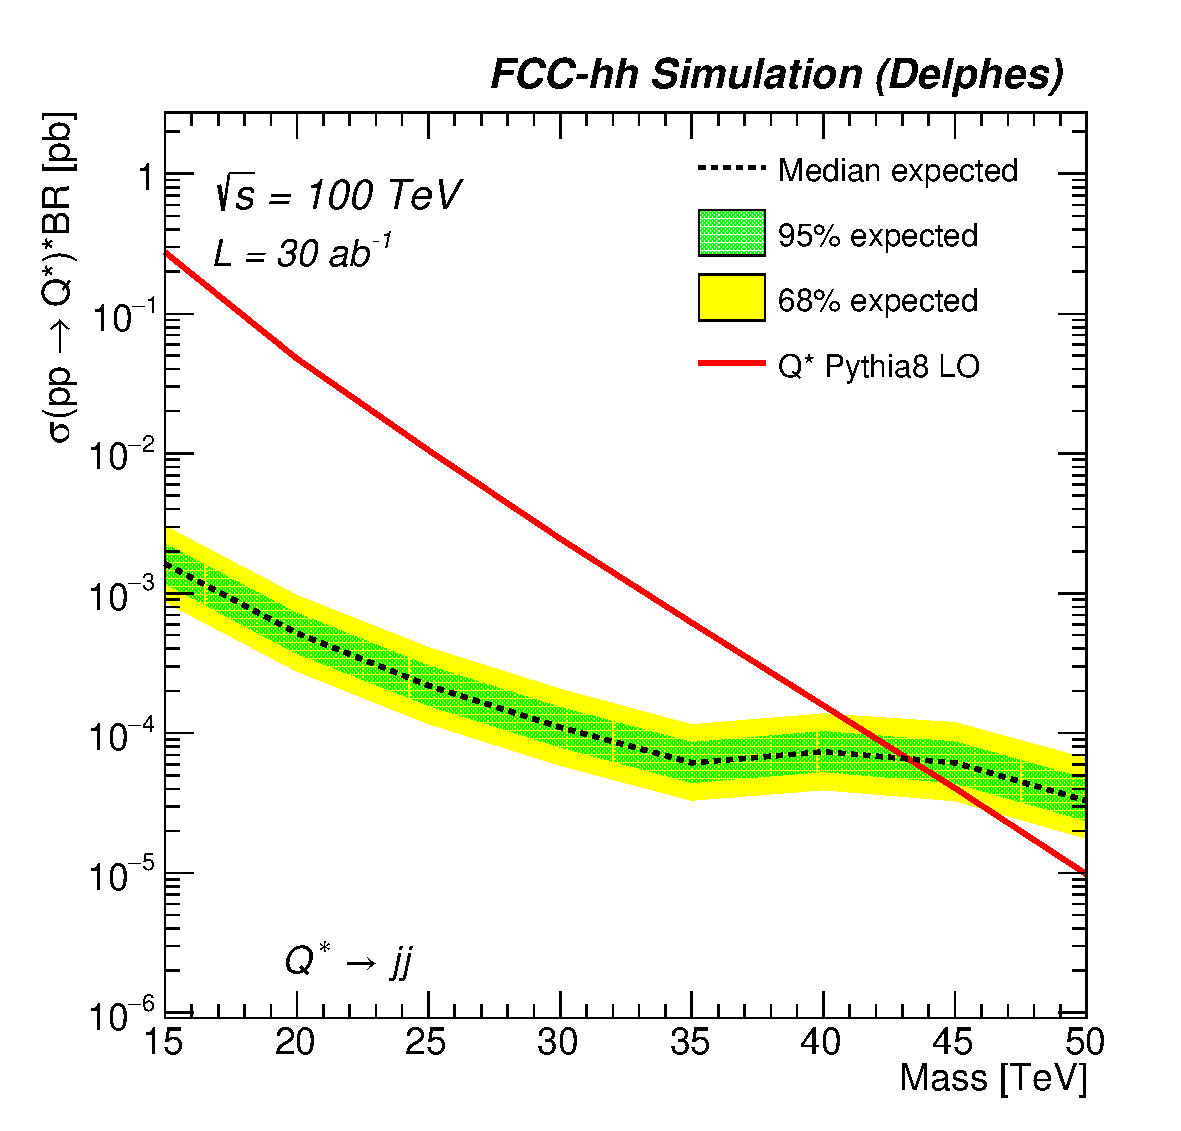
\includegraphics[width=0.32\columnwidth]{Fig/lim_Qstar_jj_fcc_v02-eps-converted-to.pdf}
  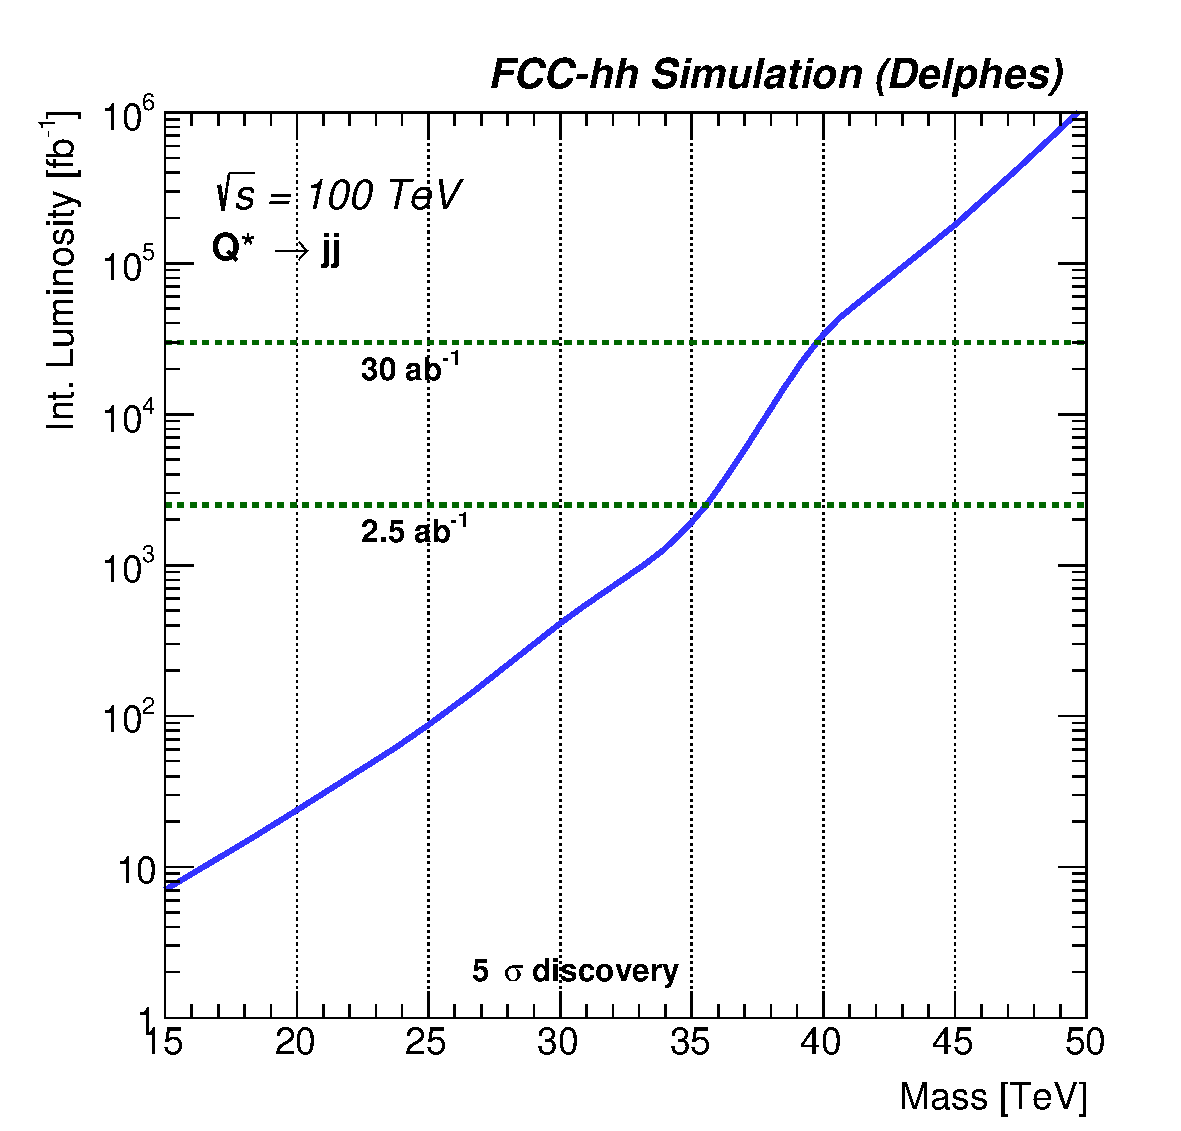
\includegraphics[width=0.32\columnwidth]{Fig/DiscoveryPotential_jj_rootStyle-eps-converted-to.pdf}
   \caption{Invariant mass distribution of the two selected jets for a 40\,TeV signal (left), 95\% CL limit versus mass (middle) and $5\sigma$ discovery reach (right).}
  \label{figure:hadronicresonances:jj}
\end{figure}

%%%%%%%%%%%%%%%%%%%%%%%%%%%%%%%%%%%%%%%%%%%%%%%%%%%%%
\subsection{The \texorpdfstring{\ttbar}{tt} final state}
\label{sec:hadtt}

To resolve the jet sub-structure, track jets are found to perform better compared to particle-flow jets, thus the \rsg\ and \Zptt\ searches are using track jets. As no lepton veto is applied, there is also some acceptance for leptonic decays and the sensitivity to semi-leptonic or \ttbar\ decays is enhanced by adding the $\metvec$ vector to the closest jet 4-momentum (among the two leading jets).
We require two jets with a $\pt$>3\,TeV and $|\eta|<3$ and $\Delta(\eta_1,\eta_2)<2.4$. Both jets must be top tagged (section~\ref{subsec:mvatagger}) by requiring multivariate tagger score larger than 0.15. In addition, the two selected high-\pt\ jets must be tagged as b-jets. Finally, to further reject QCD, we require for both jets the soft-dropped mass to be larger than 40\,GeV. Figure~\ref{figure:hadronicresonances:tt} (right) shows the di-top invariant mass distribution after the final cuts for a 20\,TeV signal. Thanks to the BDT discriminant, the largest background contribution is top pair production and the QCD contribution is now the second leading one. The middle Figure shows the 95\% CL exclusion limit obtained with 30\,ab$^{-1}$ of data and the right Figure shows the integrated luminosity required to reach a $5\sigma$ discovery as a function of the Z$^\prime$ mass. Further developments to improve the mass resolution could be considered to improve the sensitivity, but already with such wide spectrum, exclusions between 25 and 28\,TeV and discoveries between 18 and 24\,TeV are reached depending on the model (\ZpSSM or leptophobic \ZpTC).

\begin{figure}[!htb]
  \centering
   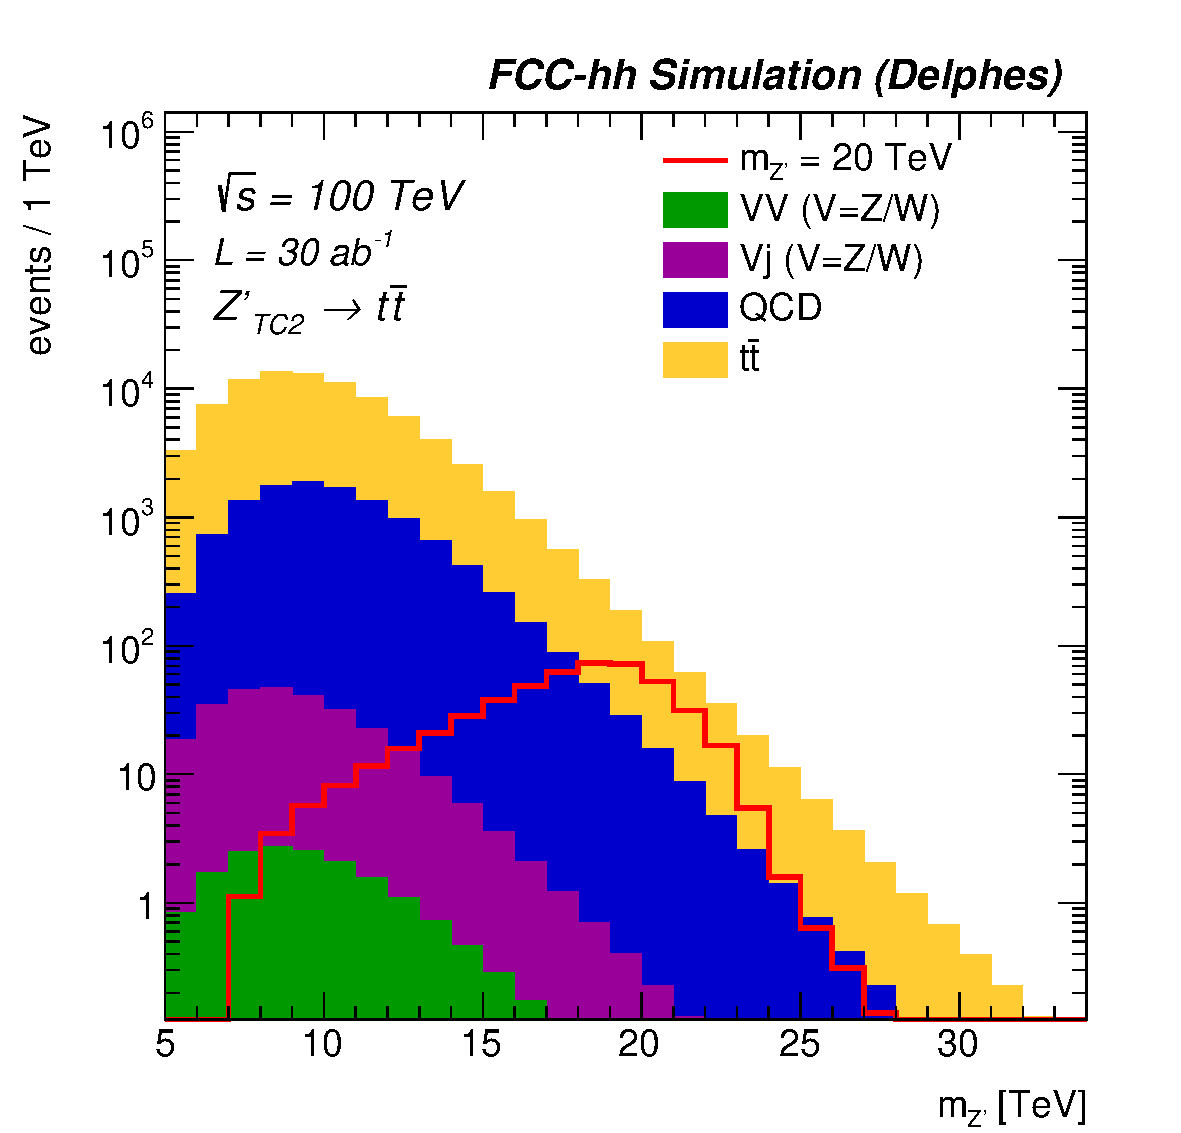
\includegraphics[width=0.32\columnwidth]{Fig/Mj1j2_pf08_MetCorr_fit_sel8_nostack_log-eps-converted-to.pdf}
   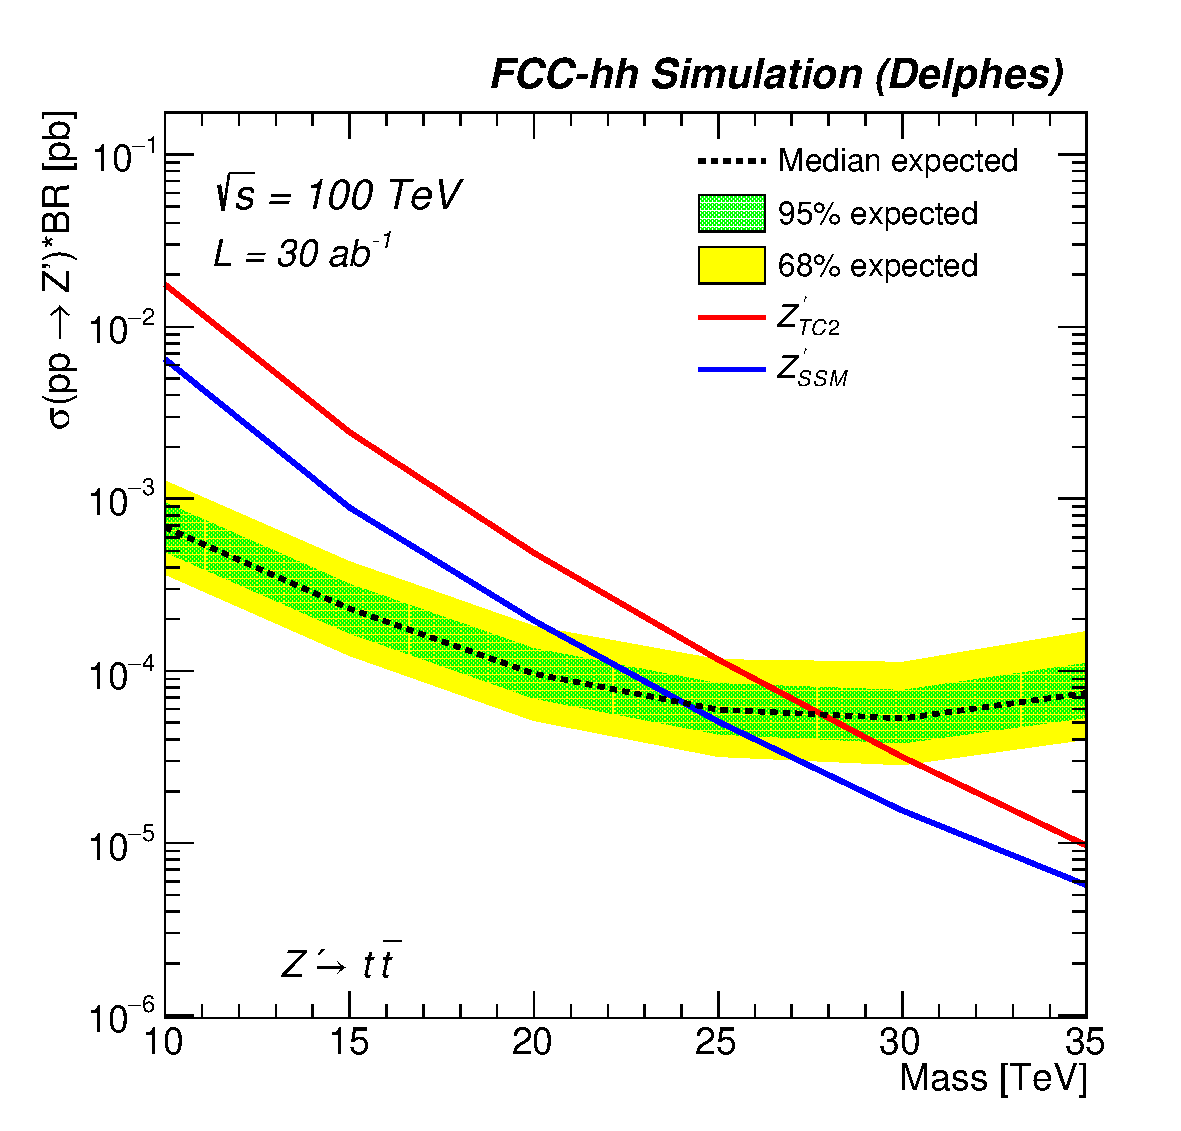
\includegraphics[width=0.32\columnwidth]{Fig/lim_Zprime_tt_fcc_v02-eps-converted-to.pdf}
   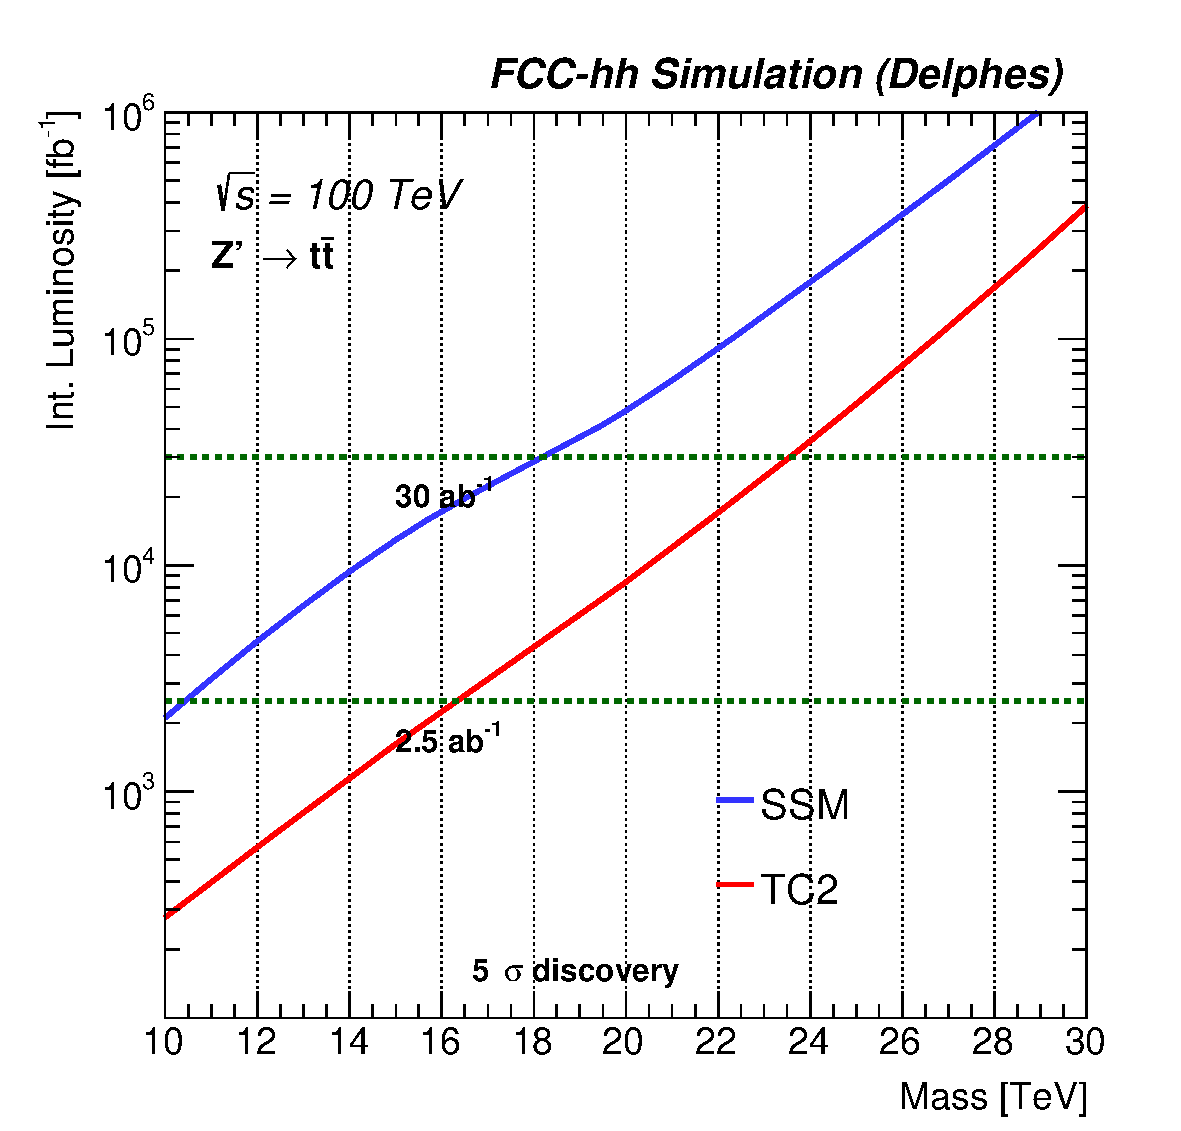
\includegraphics[width=0.32\columnwidth]{Fig/DiscoveryPotential_tt_SSM_TC2_tagger_TRFbtag_rootStyle-eps-converted-to.pdf}
  \caption{Invariant mass distribution of the two selected top-jets (left) for a 20\,TeV signal (left), 95\% CL limit versus mass (middle) and $5\sigma$ discovery reach (right).}
  \label{figure:hadronicresonances:tt}
\end{figure}


%%%%%%%%%%%%%%%%%%%%%%%%%%%%%%%%%%%%%%%%%%%%%%%%%%%%%
\subsection{The \texorpdfstring{\ww}{ww} final state}
\label{sec:hadww}
The event selection consists of two jets with a $\pt$>3\,TeV, $|\eta|<3$ and $\Delta(\eta_1,\eta_2)<2.4$. Both jets must be $W$ tagged (section~\ref{subsec:mvatagger}) by requiring multivariate tagger score larger than 0.15. Finally, to further reject QCD, we require for both jets the soft-dropped mass to be larger than 40\,GeV. Figure~\ref{figure:hadronicresonances:ww} (right) shows the di-boson invariant mass distribution after the final cuts for a 20\,TeV signal. Given the very good performance of the BDT discriminant, the QCD contribution is greatly reduced. The middle Figure shows the 95\% CL exclusion limit obtained with 30\,ab$^{-1}$ of data and the right Figure shows the integrated luminosity required to reach a $5\sigma$ discovery as a function of the Randall-Sundrum Graviton mass. Further developments to improve the W-jet/QCD could be considered to improve the sensitivity as well as combining with leptonic channels, but already with the current assumptions, exclusion of 28\,TeV and discovery of 22\,TeV is obtained.



\begin{figure}[!htb]
  \centering
  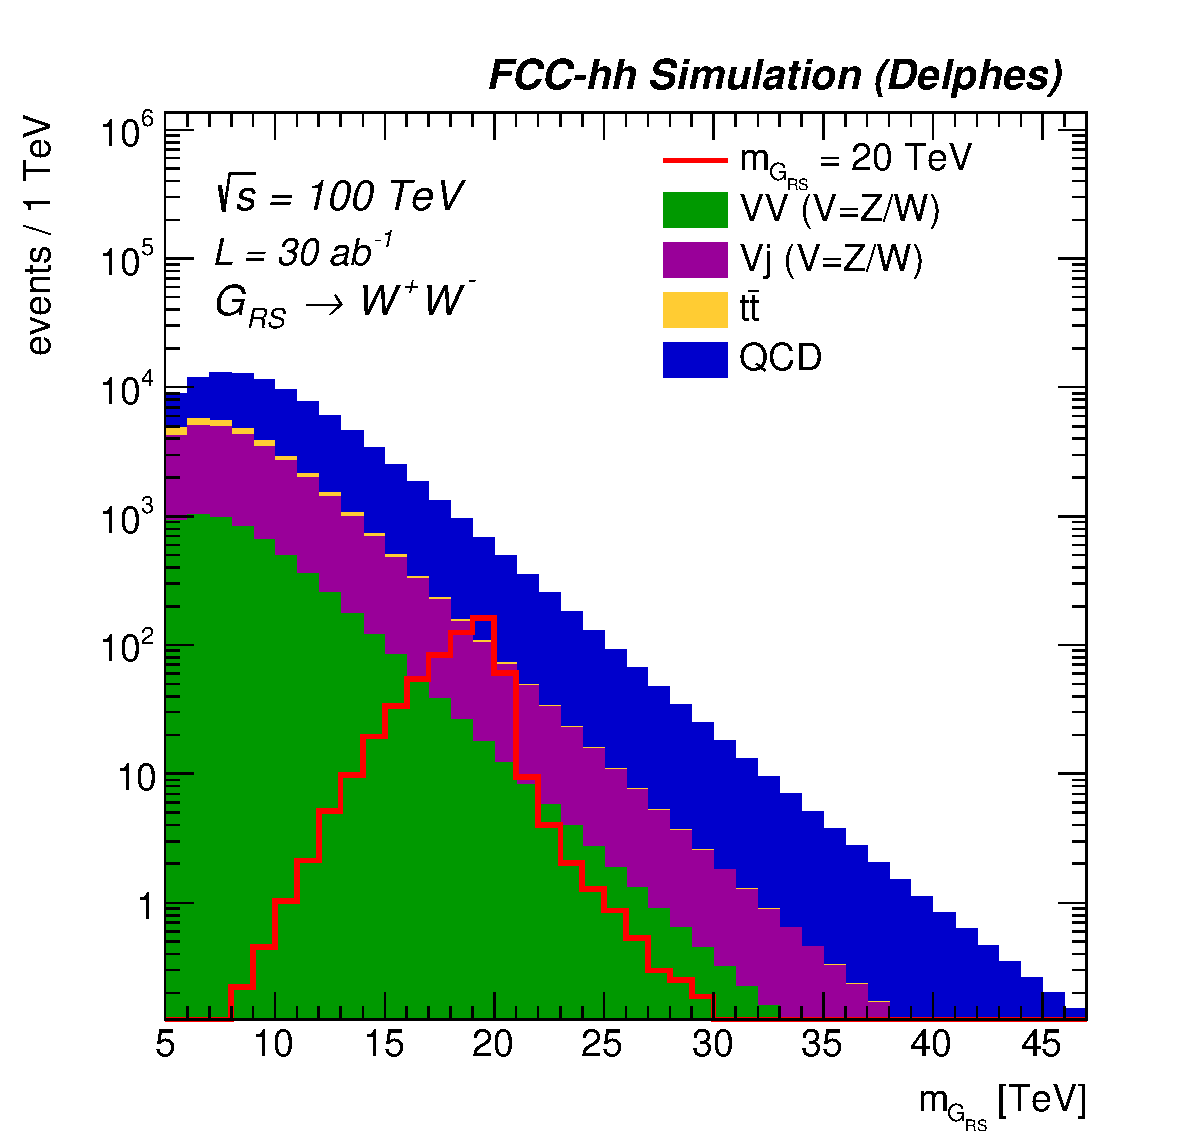
\includegraphics[width=0.32\columnwidth]{Fig/Mj1j2_pf08_fit_sel4_nostack_log-eps-converted-to.pdf}
  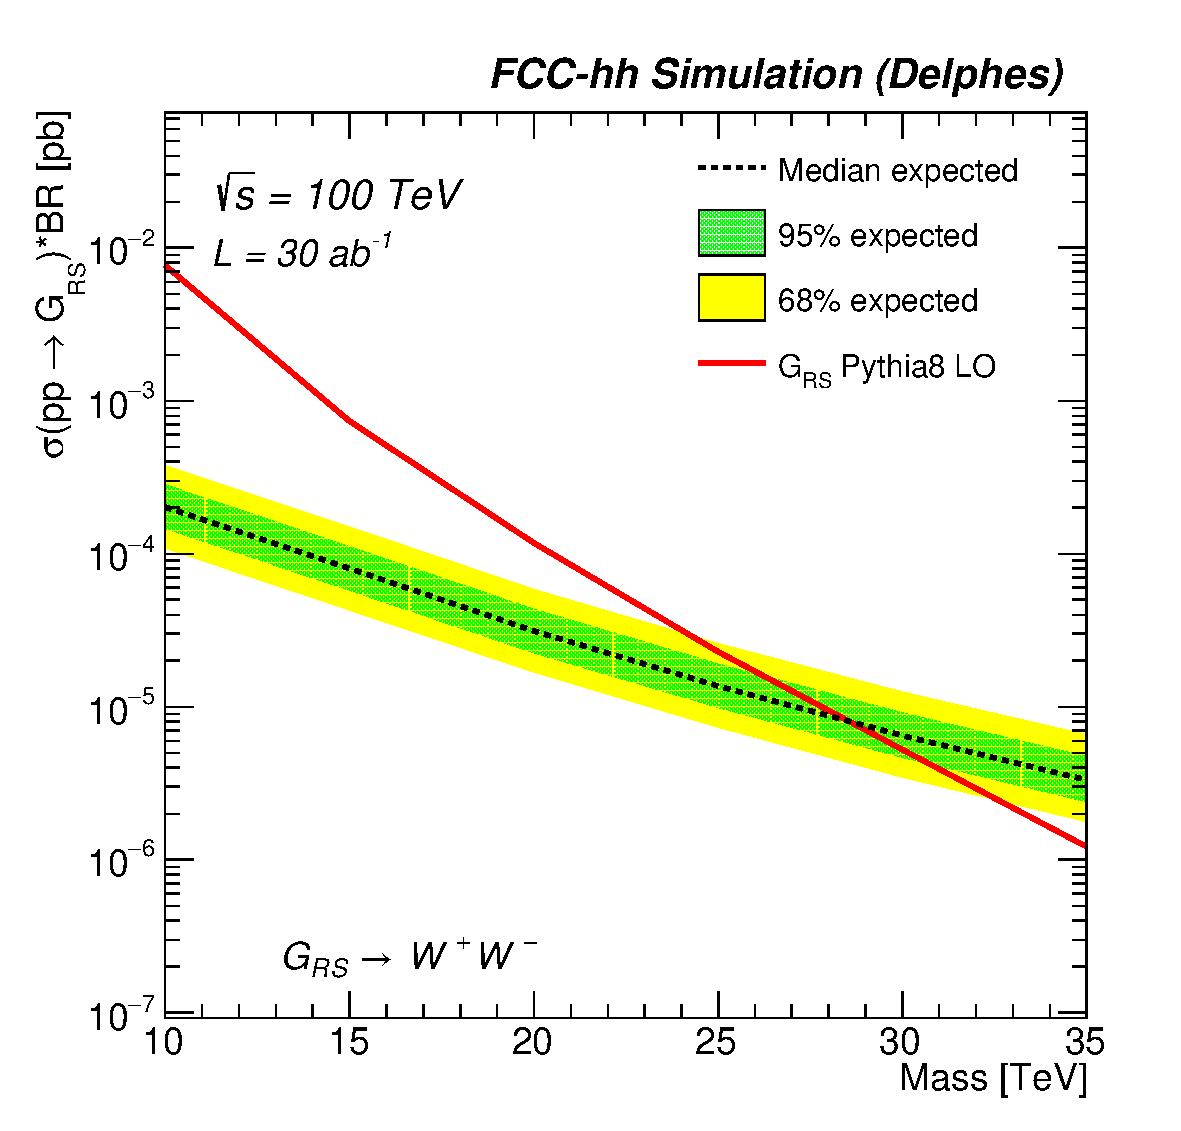
\includegraphics[width=0.32\columnwidth]{Fig/lim_RSGraviton_ww_fcc_v02-eps-converted-to.pdf}
  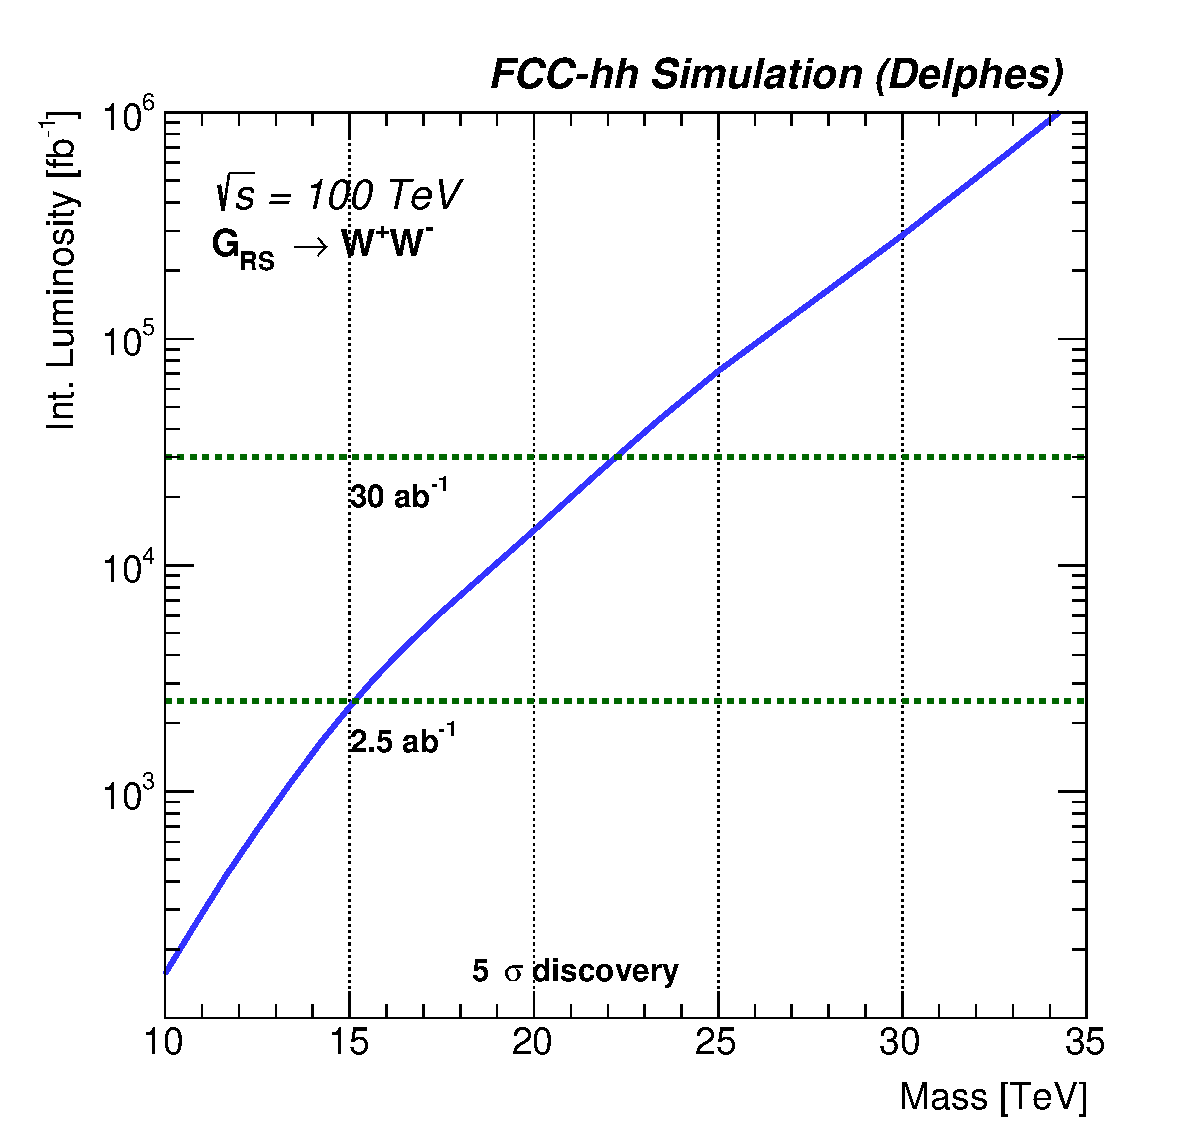
\includegraphics[width=0.32\columnwidth]{Fig/DiscoveryPotential_ww_tagger_rootStyle-eps-converted-to.pdf}
  \caption{Invariant mass distribution of the two selected W-jets for a 20\,TeV signal (left), 95\% CL limit versus mass (middle) and $5\sigma$ discovery reach (right).}
  \label{figure:hadronicresonances:ww}
\end{figure}



%%%%%%%%%%%%%%%%%%%%%%%%%%%%%%%%%%%%%%%%%%%%%%%%%%%%%
\section{Comparison with 27 TeV HE-LHC}
\label{sec:ana27tev}
The search for heavy resonances have also been study at the 27\,TeV HE-LHC. The analyses strategies remains identical to what was already presented in the previous sections, the only differences are re-optimisation of some selection thresholds to accommodate for the lower center of mass energy. The changes can be summarised as follows:
\begin{itemize}
\item \Zpee\ and \Zpmumu : lepton $p_T$ lowered from 1 to 0.5\,TeV
%\item \Zpmumu\ f.a. and t-channel LQ : leton $p_T$ lowered from  1.2 TeV to 0.75 TeV
\item \Zptata\ : mass dependent cuts changed as shown in Table~\ref{tab:leptonicresonances:tautau27}
\item \rsg, \Zptt, \qjj\ : jet $p_T$ lowered from 3 to 1\,TeV
\end{itemize}
The results are summarised in Figure~\ref{figure:resonances:summary}, together with a comparison to FCC-hh for the 95\% CL (left) and 5$\sigma$ discovery reach (right).

\begin{table}[!htb]
   \centering
\begin{tabular}{c|c|c|c}
   $\Zp$ mass [TeV] &  $\Delta \phi(\tau_1, \tau_2)$&  $\Delta R(\tau_1, \tau_2)$ & $\met$\\
  \hline
  \hline
   $2$ & > 2.4 & > 2.4 and < 3.9 & > 80 GeV\\
   $4$ & > 2.4 & > 2.7 and < 4.4 & > 80 GeV\\
   $6$ & > 2.4 & > 2.9 and < 4.4 & > 80 GeV\\
   $8$ & > 2.6 & > 2.9 and < 4.6 & > 80 GeV\\
  $10$ & > 2.8 & > 2.9 and < 4.1 & > 60 GeV\\
%  $12$ & > 2.8 & > 3.0 and < 3.6 & > 60 GeV\\
%  $14$ & > 3.0 & > 3.0 and < 3.3 & > 60 GeV\\
  \end{tabular}
  \caption{Mass dependent cuts optimised to maximise the sensitivity for the \Zptata\ resonance search.}
  \label{tab:leptonicresonances:tautau27}
\end{table}




\begin{figure}[!htb]
  \centering
  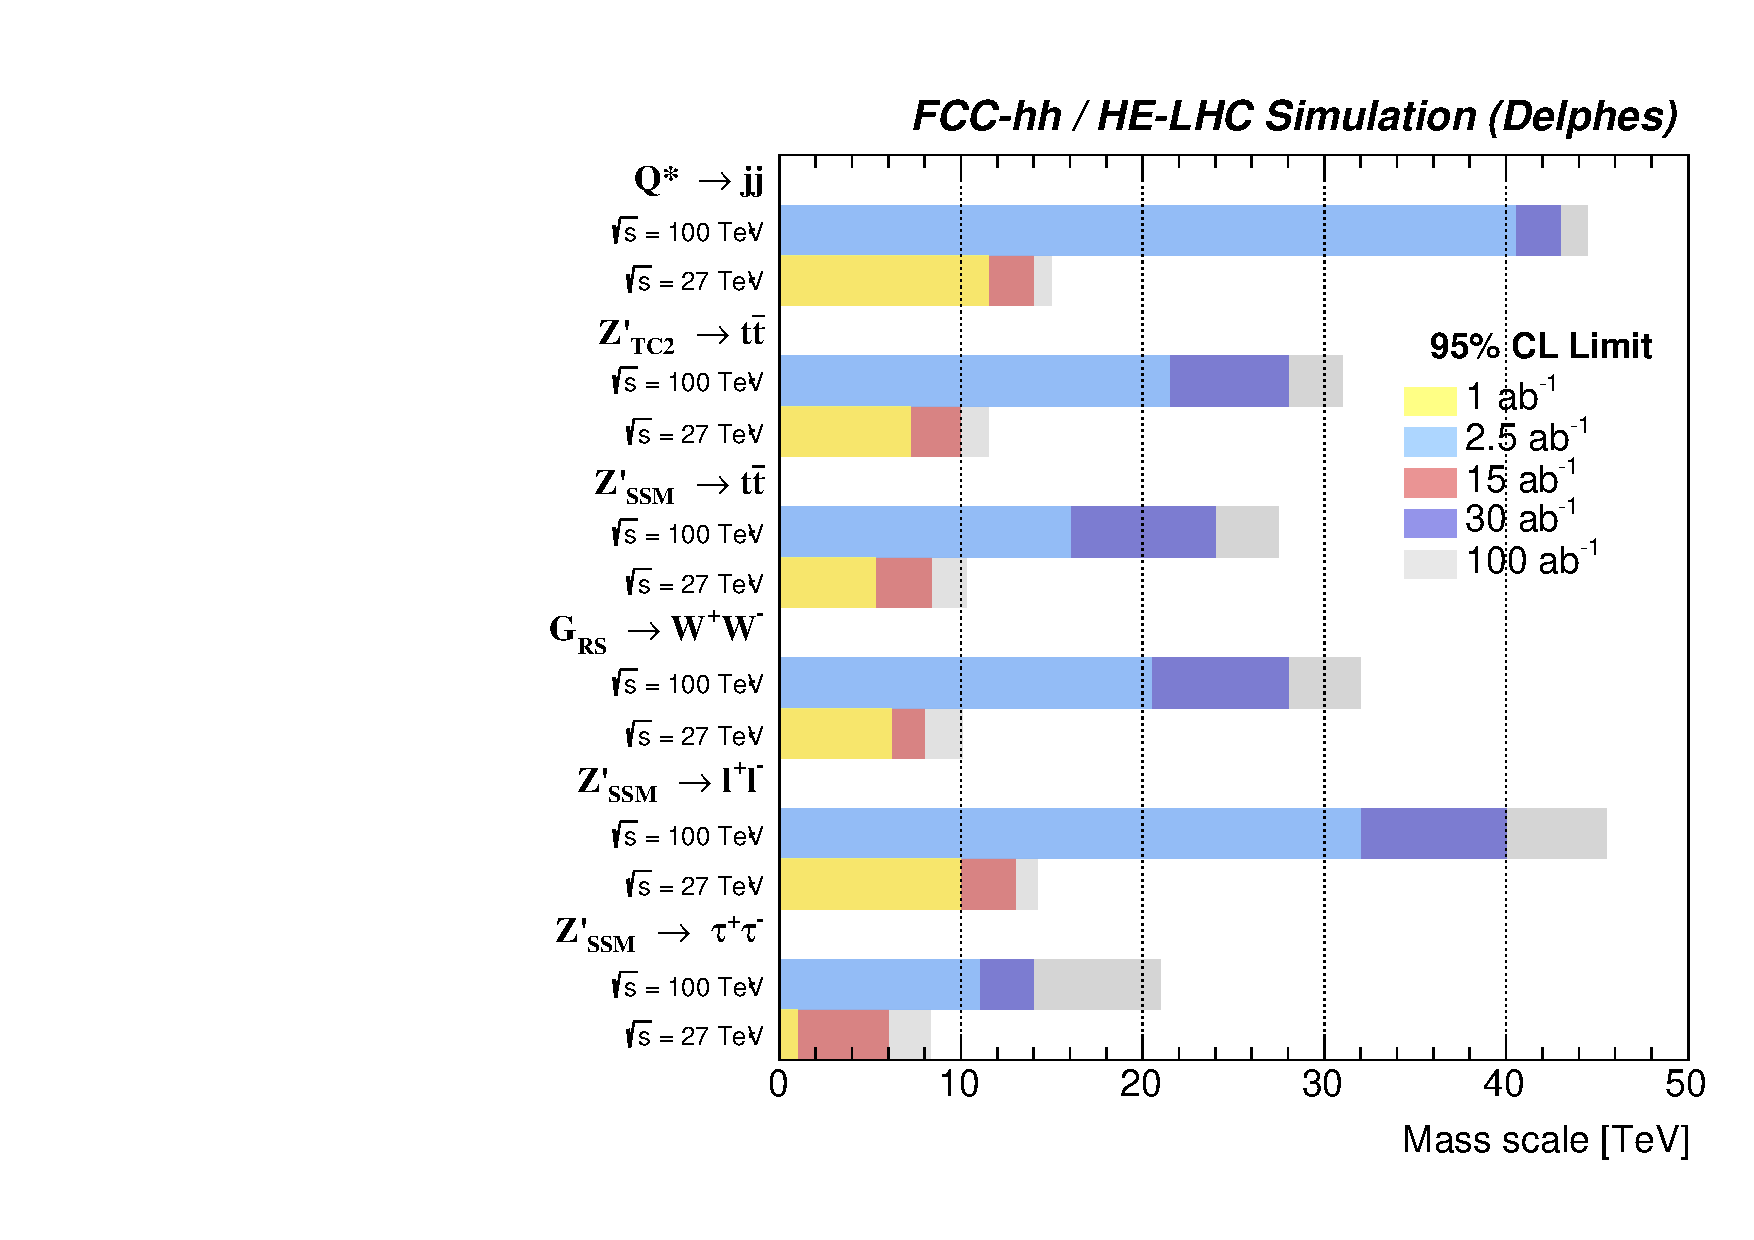
\includegraphics[width=0.49\columnwidth]{Fig/summaryLimit.pdf}
  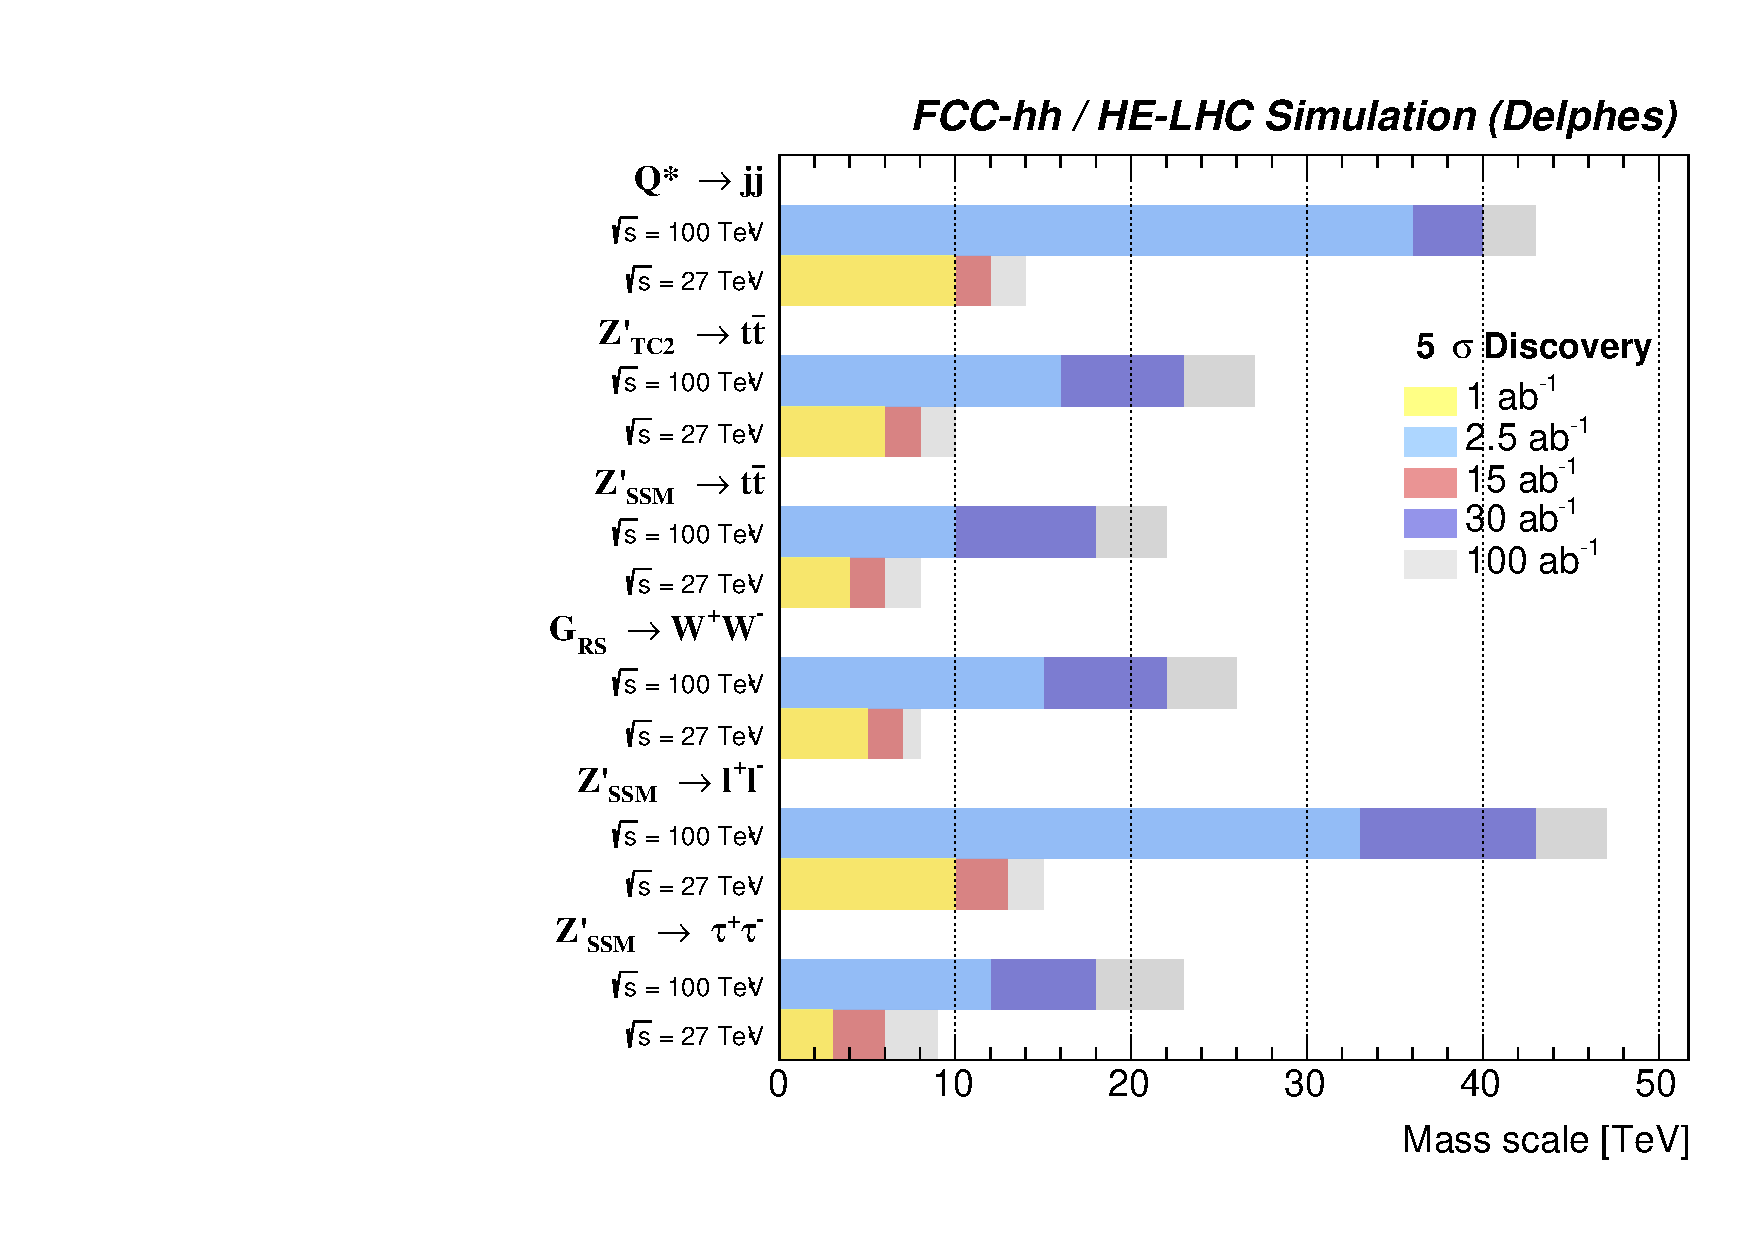
\includegraphics[width=0.49\columnwidth]{Fig/summaryDisco.pdf}
  \caption{Summary of the 95\% CL limits (left) and $5\sigma$ discovery reach (right) as a function of the resonance mass for different luminosity scenario of FCC-hh and HE-LHC.}
  \label{figure:resonances:summary}
\end{figure}

%\begin{table}[!htb]\centering
%\begin{tabular}{|l|c|c|c|}
%\hline
%analysis   & \multicolumn{3}{c|}{HE-LHC (FCC-hh)} \\
%           & Limit [TeV] & Disco [TeV]   & Disco [TeV] \\
%           &  15 (30) ab$^{-1}$ & 1 (2.5) ab$^{-1}$ & 15 (30) ab$^{-1}$ \\
%\hline
%\Zpll\ (l=e,$\mu$) & 13 (40) & 10 (33) & 13 (43) \\
%\Zptata       &  6 (14) &  3 (12) &  6 (18) \\
%%\Zpmumu\ f.a. &  4 (25) &  - (10) &  2 (19) \\
%\Zptt         & 10 (28) &  6 (16) &  8 (23) \\
%\rsg          &  8 (28) &  5 (15) &  7 (22) \\
%\qjj          & 14 (43) & 10 (36) & 12 (40) \\
%\hline
%\end{tabular}
%\caption{95\% CL limits and 5$\sigma$ discovery reach comparison between HE-LHC and FCC-hh. The numbers in parenthesis are the FCC numbers. \CH{TO BE REMOVED if decide that summary plots are better}}
%\label{tab:27vs100}
%\end{table}




%%%%%%%%%%%%%%%%%%%%%%%%%%%%%%%%%%%%%%%%%%%%%%%%%%%%%
\section{Characterisation of a Z' discovery}
\label{sec:zprimedisc}

%%%%%%%%%%%%%%%%%%%%%%%%%%%%%%%%%%%%%%%%%%%%%%%%%%%%%
\subsection{Context of the study}
%\paragraph*{Context of the study}
It is still legitimate to assume that a heavy resonance could be seen at the end of HL-HLC. If that is the case a new collider with higher energy
in the \com is needed to study its properties as too few events will be available at \sqrtslhc. In this section we present the discrimination potential between six $Z'$ models of a High Energy LHC (HE-LHC) with an assumed \com energy of 27\,TeV and an integrated luminosity of \intlumihelhc. Under the assumption that these $Z'$'s decay only to SM particles, we show that there are sufficient observables to perform this model differentiation in most cases.

%%%%%%%%%%%%%%%%%%%%%%%%%%%%%%%%%%%%%%%%%%%%%%%%%%%%%
\subsection{Bounds from HL-LHC}
%\paragraph*{Bounds from HL-LHC}
As a starting point it is needed to estimate what are, for $\sqrt s=14$\,TeV, the typical exclusion/discovery reaches for standard reference $Z'$ models assuming \intlumihllhc\ employing only the $e^+e^-$ and $\mu^+\mu^-$ channels. To address this and the other questions below we will use the same set of $Z'$ models as employed
in Ref.~\cite{Rizzo:2014xma} and mostly in Ref.~\cite{Han:2013mra}, both of which we will refer to frequently. We employ the MMHT2014 NNLO PDF set~\cite{Harland-Lang:2014zoa}
throughout with an appropriate constant $K$-factor (=1.27) to account for higher order QCD corrections. The production cross section times leptonic branching fraction is shown in Figure~\ref{fig:pheno:toy} (left) for these models at \sqrtslhc\ in the narrow width approximation (NWA). It has been and will be assumed here that these $Z'$ states only decay to SM particles.


\begin{figure}[htbp]
  \centering
    \includegraphics[trim={2cm 2cm 2cm 2cm},clip,width=0.45\columnwidth]{Fig/zp14tev-ref.pdf}
    \includegraphics[trim={2cm 2cm 2cm 2cm},clip,width=0.45\columnwidth]{Fig/zp27tev-ref.pdf}
    \caption{Left: $\sigma B_l$ in the NWA for the $Z'$ production at the $\sqrt s=14$\,TeV LHC as functions of the $Z'$ mass: SSM(red), LRM (blue), $\psi$(green), $\chi$(magenta),
$\eta$(cyan), I(yellow). (Right) $\sigma B_l$ of $Z'$ in models described in (left) at $\sqrt s=27$\,TeV.}
\label{fig:pheno:toy}
\end{figure}

Using the present ATLAS and CMS results at 13\,TeV,~\cite{Aaboud:2017buh} and~\cite{Sirunyan:2018exx}, it is straightforward to estimate by extrapolation the
exclusion reach at \sqrtslhc\ using the combined $ee+\mu\mu$ final states. This is given in the first column of Table~\ref{tab:pheno:spec}. For discovery, only the $ee$ channel is used due to poor $\mu\mu$-pair invariant mass resolution near $M_{Z'}=6$\,TeV. Estimates of the $3\sigma$ evidence and $5\sigma$
discovery limits are also given in Table~\ref{tab:pheno:spec}. Based on these results, we will assume in our study below that we are dealing with a $Z'$ of mass 6\,TeV. Figure~\ref{fig:pheno:toy} (right) shows the NWA cross sections for the same set of models but now at \sqrtshelhc\ with \intlumihelhc. We note that very large statistical samples will be available for the case of $M_{Z'}=6$\,TeV
for each dilepton channel.

%
\begin{table}
\centering
\begin{tabular}{c|c|c|c}

  Model &   95$\%$ \cl  &  $3\sigma$  & $5\sigma$   \\
\hline
\hline
SSM    &     6.62     &  6.09    &  5.62     \\
LRM    &   6.39     & 5.85     & 5.39  \\
$\psi$    &  6.10   & 5.55   & 5.07  \\
$\chi$   &  6.22    & 5.68    & 5.26   \\
$\eta$   &  6.15     &  5.59  &  5.16   \\
~I        & 5.98   &  5.45   &  5.05  \\
\end{tabular}
\caption{ Mass reach for several $Z'$ models at \sqrtslhc\ with \intlumihllhc. }
\label{tab:pheno:spec}
\end{table}
%

%%%%%%%%%%%%%%%%%%%%%%%%%%%%%%%%%%%%%%%%%%%%%%%%%%%%%
%\paragraph*{Definition of the discriminating variables}
\subsection{Definition of the discriminating variables}
\label{par:vardef}

The various $Z'$ models can be disentangled with the help of 3 inclusive observables: the production cross section times leptonic branching fraction $\sigma B_l$, the forward-backward asymmetry $A_{FB}$ and the rapidity ratio $r_y$. The variable $A_{FB}$ can be seen as an estimate of the charge asymmetry
\begin{equation}
A_{FB} = A_C =  \frac{\sigma(\Delta|y| > 0) - \sigma(\Delta|y| < 0)}{\sigma(\Delta|y| > 0) + \sigma(\Delta|y| < 0)},
\end{equation}
where $\Delta|y| = |y_l| - |y_{\bar{l}}|$. It has been checked that this definition is equivalent to defining
\begin{equation}
A_{FB} = \frac{\sigma_F - \sigma_B}{\sigma_F + \sigma_B},
\end{equation}
with $\sigma_F = \sigma (cos\theta^{*}_{cs})>0$ and $\sigma_B = \sigma (cos\theta^{*}_{cs})<0$ where $\theta^*_{cs}$ is the Collins-Soper frame angle. The variable $r_y$ is defined as the ratio of central over forward events:
\begin{equation}
r_y = \frac{\sigma(|y_{Z'}| < y_1)}{\sigma(y_1 < |y_{Z'}| <y_2)},
\end{equation}
where $y_1=0.5$ and $y_2=2.5$.

%%%%%%%%%%%%%%%%%%%%%%%%%%%%%%%%%%%%%%%%%%%%%%%%%%%%%
%\paragraph*{Model discrimination}
\subsection{Model discrimination}

The model discrimination presented in this section has been performed assuming the HE-LHC detector parametrisation~\cite{hlhelhc_web} in \delphes~\cite{deFavereau:2013fsa}. In such a detector, muons at $\eta \approx 0$ are assumed to be reconstructed with a resolution $\sigma(p)/p \approx 7\%$ for $\pt~=~3$\,TeV.

%%%%%%%%%%%%%%%%%%%%%%%%%%%%%%%%%%%%%%%%%%%%%%%%%%%%%
%\subparagraph*{Leptonic final states}
\subsubsection{Leptonic final states}
\label{par:lepana}

The potential for discriminating various $Z'$ models is first investigated using the leptonic $ee$ and $\mu\mu$ final states only. The signal samples for the 6 models and the Drell-Yan backgrounds have been generated with \py~\cite{Sjostrand:2014zea} including the interference between the signal and background. The $Z'$ decays assume lepton flavour universality. For a description of the event selection and a discussion of the discovery potential in leptonic final states for the list of $Z'$ models being discussed here, the reader should refer to Section~\ref{sec:lep}. We simply point out here that with \intlumihelhc\,, all $Z'$ models with $m_{Z'}~\lesssim~10$\,TeV can be excluded at \sqrtshelhc.

Figure~\ref{fig:ana:res} (left) shows the correlated predictions for the $A_{FB}$ and the rapidity ratio $r_y$ observables defined previously for these six models given the above assumptions. Although the interference with the SM background was included in the simulation, its effect is unimportant due to the narrowness of the mass window around the resonance that was employed. Furthermore, the influence of the background uncertainty on the results has been found to have little to no impact on the model discrimination potential. Therefore the displayed errors on $A_{FB}$ and $r_y$ are of statistical origin only. The results show that apart from a possible near degeneracy in models $\psi$ and $\eta$, a reasonable $Z'$ model separation can indeed be achieved.

Using a profile likelihood technique, the signal strength $\mu$, or equivalently, $\sigma B_l$, can be fitted together with its corresponding error using the the di-lepton invariant mass shape. The quantity $\sigma B_l$ and its total estimated uncertainty is shown in Figure~\ref{fig:ana:res} (center) as a function of the integrated luminosity. The $\sigma B_l$ measurement seems to be able to resolve the degeneracy between the $\psi$ and $\eta$ models with \intlumihelhc. It should be noted however that since the cross-section can easily be modified by an overall rescaling of the couplings, further handles will be needed for a convincing discrimination.

\begin{figure}[!htb]
  \centering
   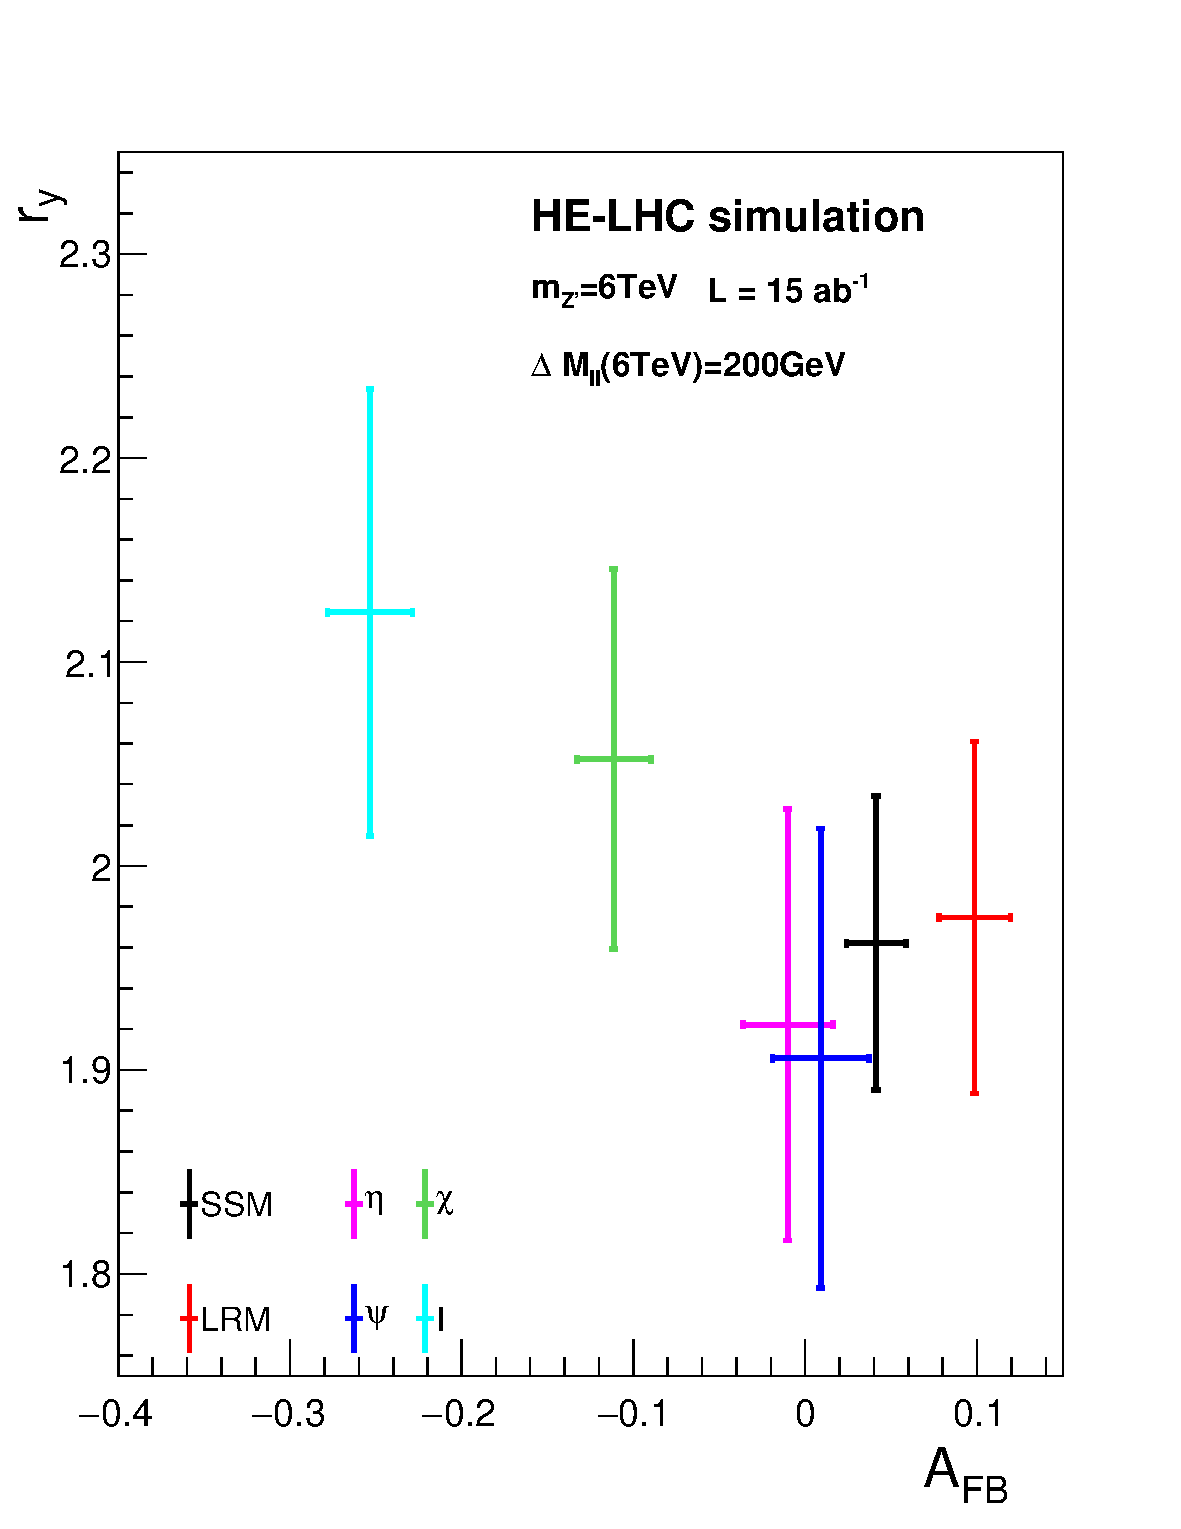
\includegraphics[width=0.30\columnwidth]{Fig/ry_afb_200GeV_eta2p5_interf-eps-converted-to.pdf}
   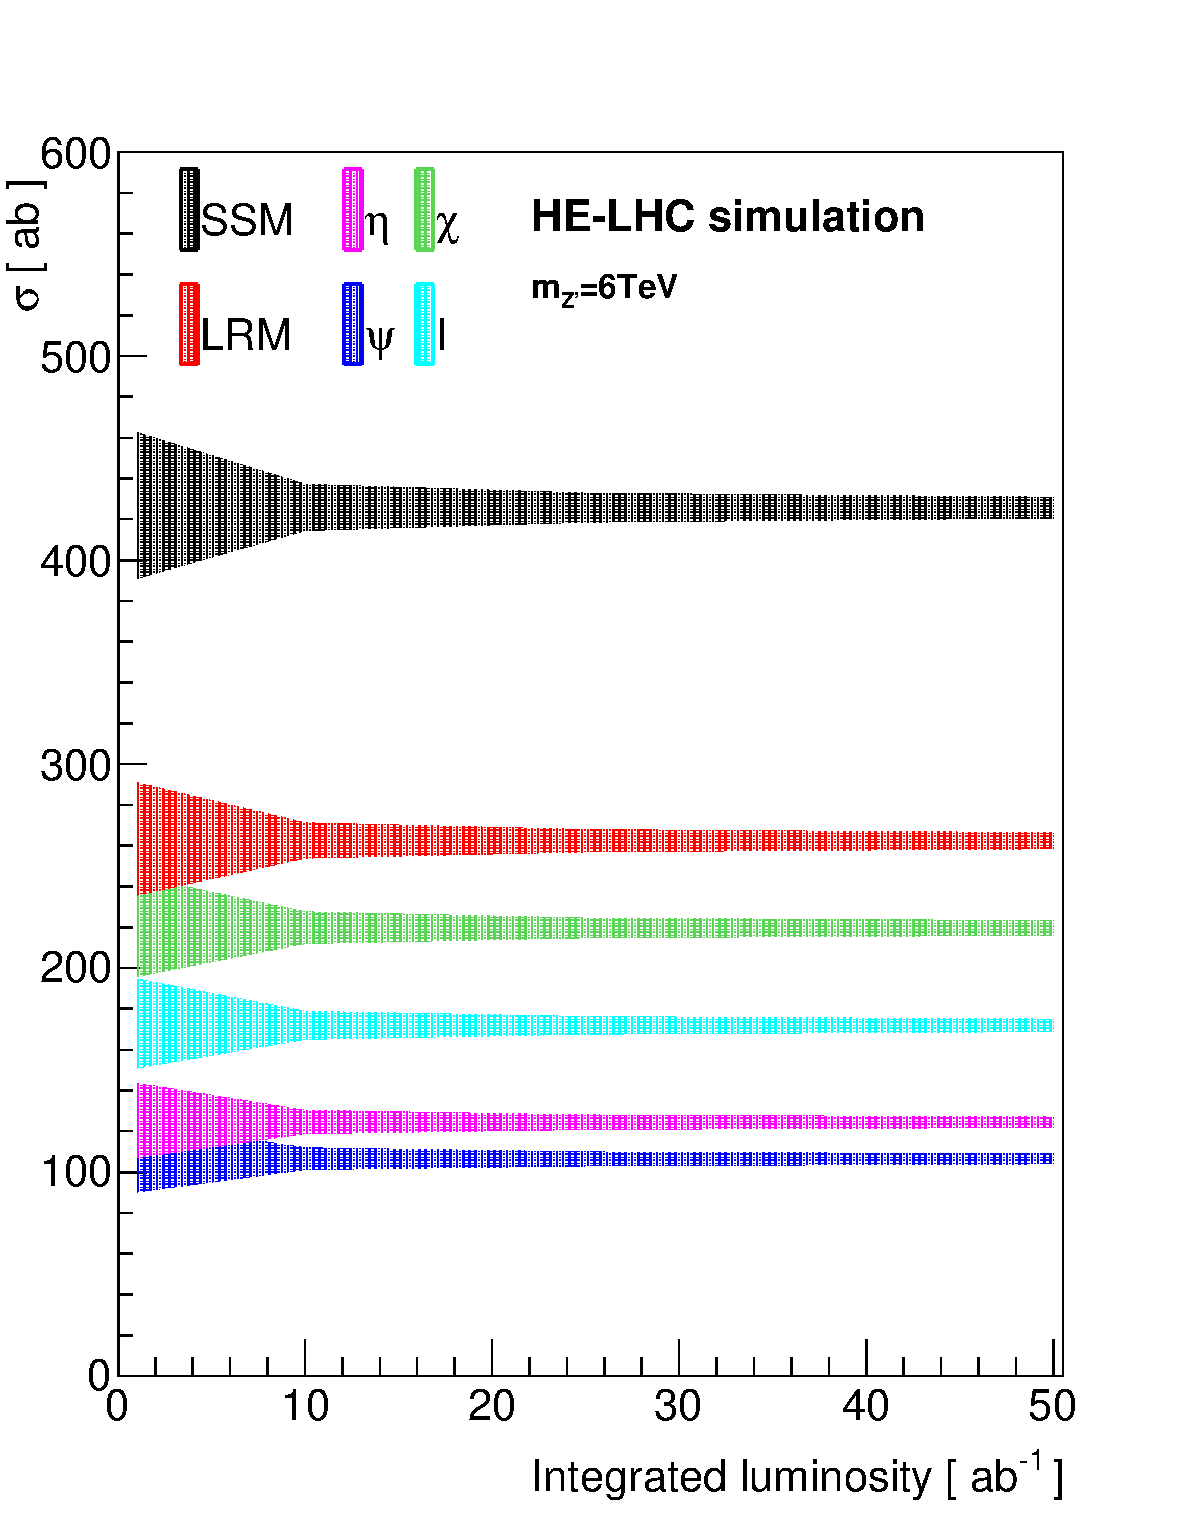
\includegraphics[width=0.30\columnwidth]{Fig/sigma_vs_lumi-eps-converted-to.pdf}
   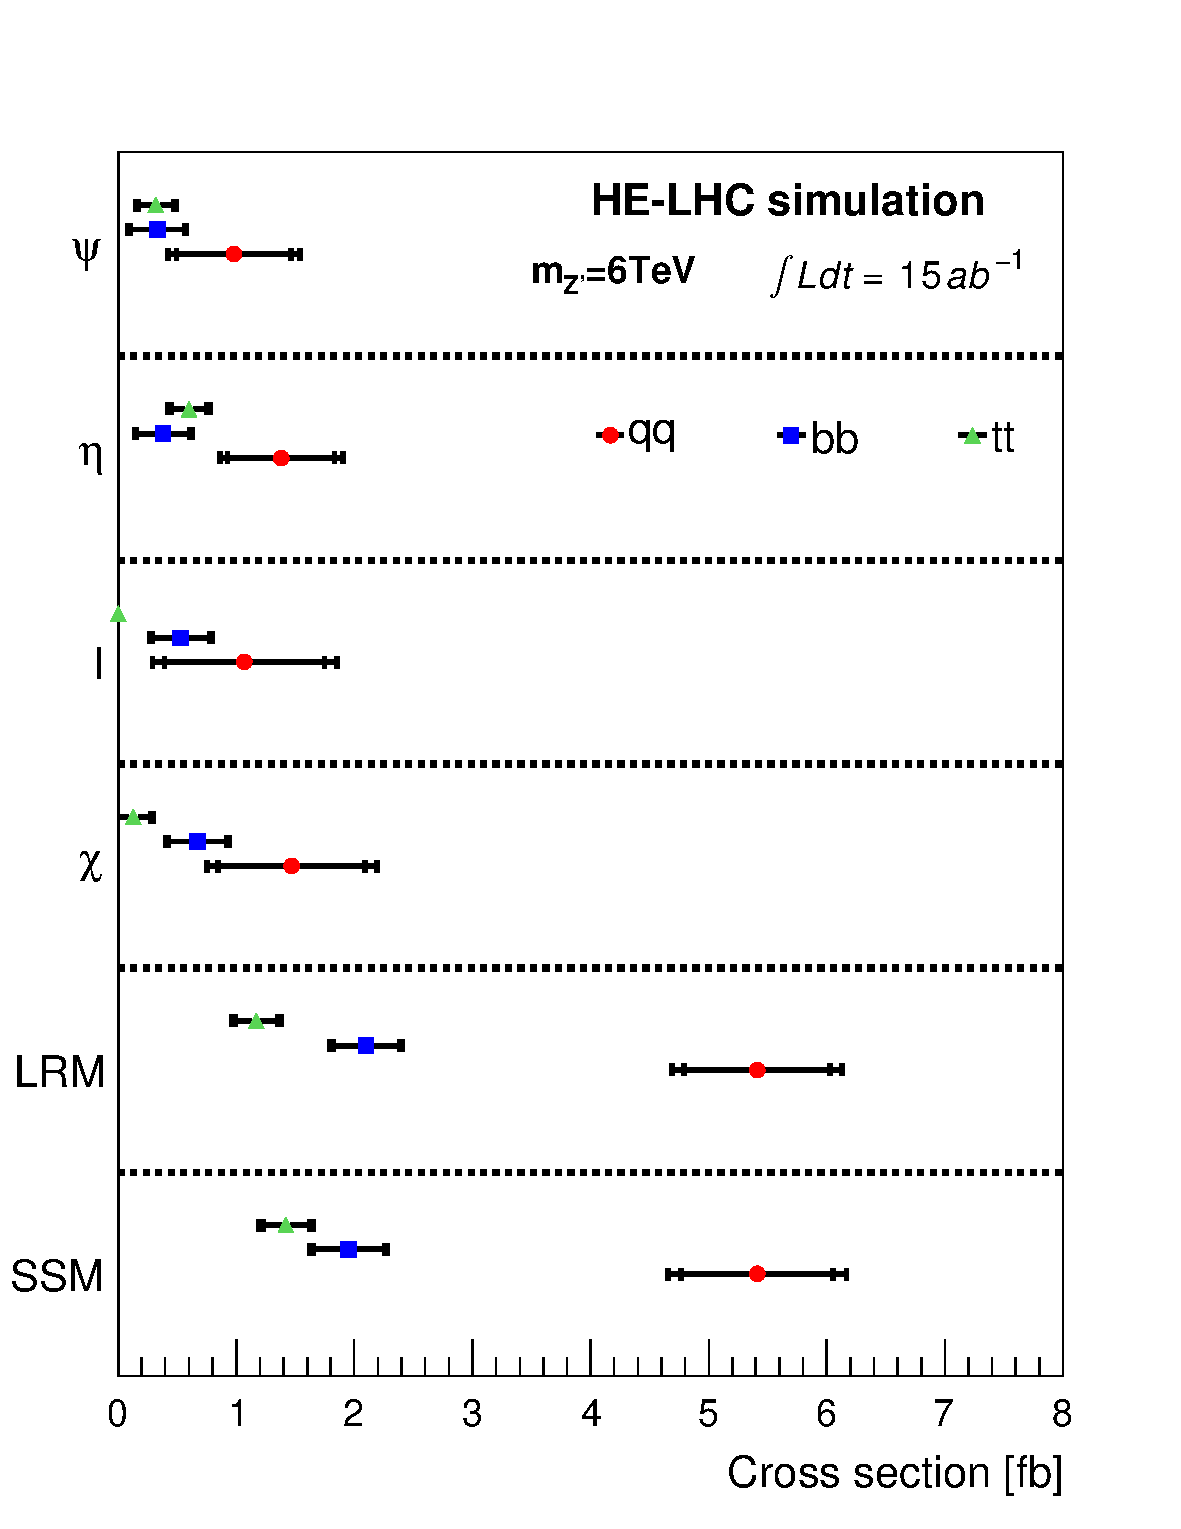
\includegraphics[width=0.30\columnwidth]{Fig/Zp_branching_6TeV_15ab-eps-converted-to.pdf}
  \caption{Left: Scatter plot of $r_y$ versus $A_{FB}$ with 200~GeV and mass window. The full interference is included. Center: Fitted signal cross-section together with its corresponding error versus integrated luminosity. Right: Fitted cross-section of the three hadronic analyses. Statistical and full uncertainties are shown on each point.}
  \label{fig:ana:res}
\end{figure}

%%%%%%%%%%%%%%%%%%%%%%%%%%%%%%%%%%%%%%%%%%%%%%%%%%%%%
%\subparagraph*{Hadronic final states}
\subsubsection{Hadronic final states}
\label{par:hadana}

Model discrimination can be improved by including an analysis involving three $Z'$ addition hadronic final states: $t\bar{t}$, $b\bar{b}$ and $q\bar{q}$, where $q=u,d,c,s$. The sample production and event selection for the $t\bar{t}$, $q\bar{q}$ final states has been described to some extent in Section~\ref{sec:hadronic}. We simply remind the reader that the analysis involves requiring the presence of two central high $\pt$ jets. In order to ensure complete orthogonality between the various final states, jets are required to be tagged as follows. In the $Z' \rightarrow t\bar{t}$ analysis both jets should be \emph{top-tagged}. For the $Z' \rightarrow b\bar{b}$ final state both jets are required to be \emph{b-tagged} and we veto events containing at least one top-tagged jet. Finally, in the $Z' \rightarrow q\bar{q}$ analysis, we veto events that contain at least one b-tagged or top-tagged jet.

Figure~\ref{fig:ana:res} (right) summarises the discrimination potential in terms of fitted cross-section of the different models considering the three aforementionned hadronic decays, $t\bar{t}$,  $b\bar{b}$ and $q\bar{q}$. An good overall discrimination among the various models can be achieved using all possible final states. For example, the SSM and $\psi$ models, which have very close predictions for $r_y$ and $A_{FB}$, have measurably different fractions of $t\bar{t}$ or $b\bar{b}$ final states. We note however that the degeneracy between $\eta$ and $\psi$ can only be partially resolved resolved at $\approx~1~\sigma$ by exploiting the difference in $t\bar{t}$ yield.

%%%%%%%%%%%%%%%%%%%%%%%%%%%%%%%%%%%%%%%%%%%%%%%%%%%%%
%\paragraph*{Conclusion}
\subsection{Interpretation of the results}
In this section we studied the discrimination potential of six $Z'$ models at High Energy LHC (HE-LHC) with an assumed \com energy of 27\,TeV and an integrated luminosity of \intlumihelhc. The exercise has been performed assuming the evidence of an excess observed at \sqrtslhc\ at a mass $m_{Z'}\approx~6$\,TeV. Overall it was found that it is possible to distinguish among most models. Finally, it should be noted that further studies, perhaps employing 3-body decay modes or associated Z' production will be clearly in case of discovery to further characterize the resonance properties.


%%%%%%%%%%%%%%%%%%%%%%%%%%%%%%%%%%%%%%%%%%%%%%%%%%%%%
\section{Flavour anomaly inspired Z' models sensitivity at the FCC-hh}
\label{sec:zprimeflav}
LHCb measurements in $B\rightarrow~K^*\mu~+\mu~-$ decays are somewhat discrepant with SM predictions~\cite{Aaij:2014ora,Aaij:2017vbb}. They may be harbingers of new physics at an energy scale potentially accessible to direct discovery. The "naive" flavour anomaly model $Z'$ from~\cite{Allanach:2017bta} is studied in this section. The only difference with respect to the selection strategy described in section~\ref{sec:lepee} is the increase of lepton momentum threshold from 1 to 1.2 TeV. Figure~\ref{figure:leptonicresonances:resultsmumu_flav} shows the invariant mass of the $\mu^+\mu^-$ system (left), the 95\% CL exclusion limit obtained (middle) and the integrated luminosity required to reach a $5\sigma$ discovery as a function of the mass of the $\mu^+\mu^-$ system (right). Even if the assumed muon momentum resolution in~\cite{Allanach:2017bta} is too optimistic, the results we find with more realistic performances are in agreement.


\begin{figure}[!htb]
  \centering
  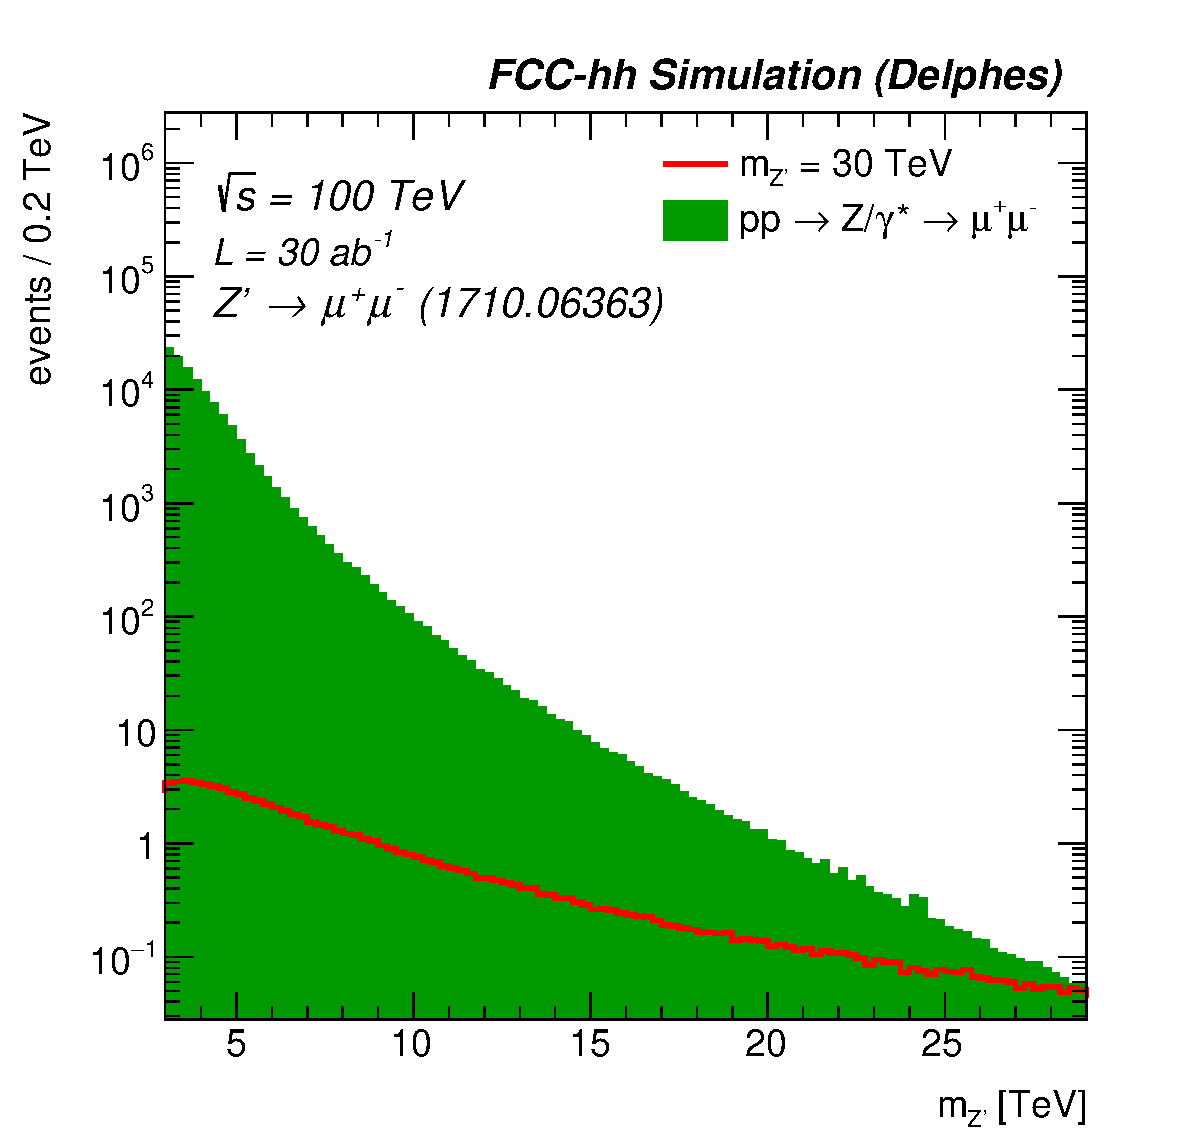
\includegraphics[width=0.32\columnwidth]{Fig/mzp_sel0_nostack_log_FA-eps-converted-to.pdf}
  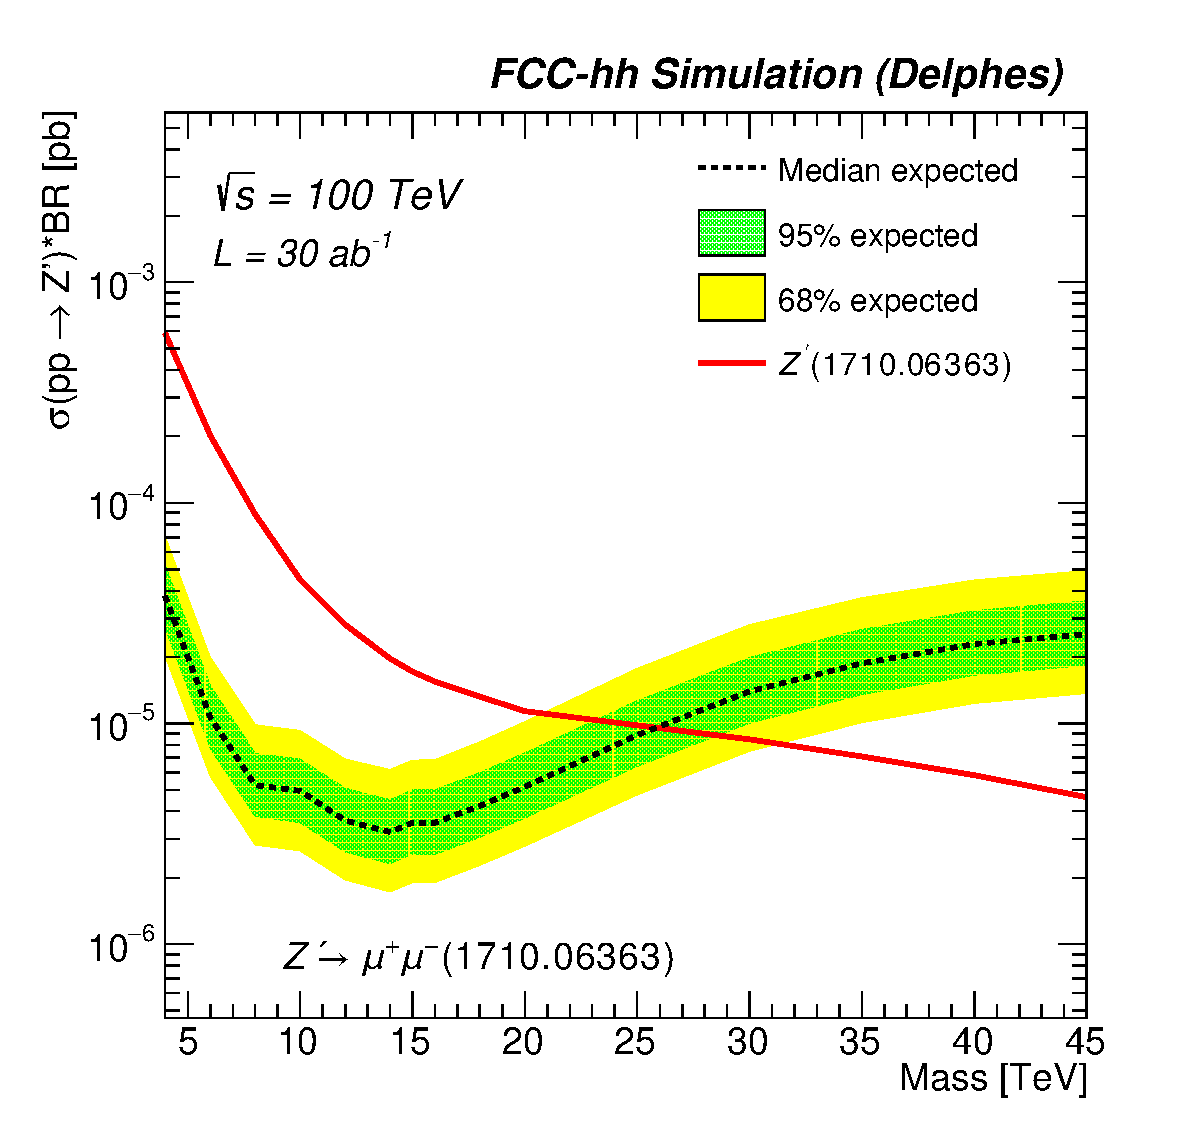
\includegraphics[width=0.32\columnwidth]{Fig/lim_Zprime_mumu_ano_fcc_v02-eps-converted-to.pdf}
  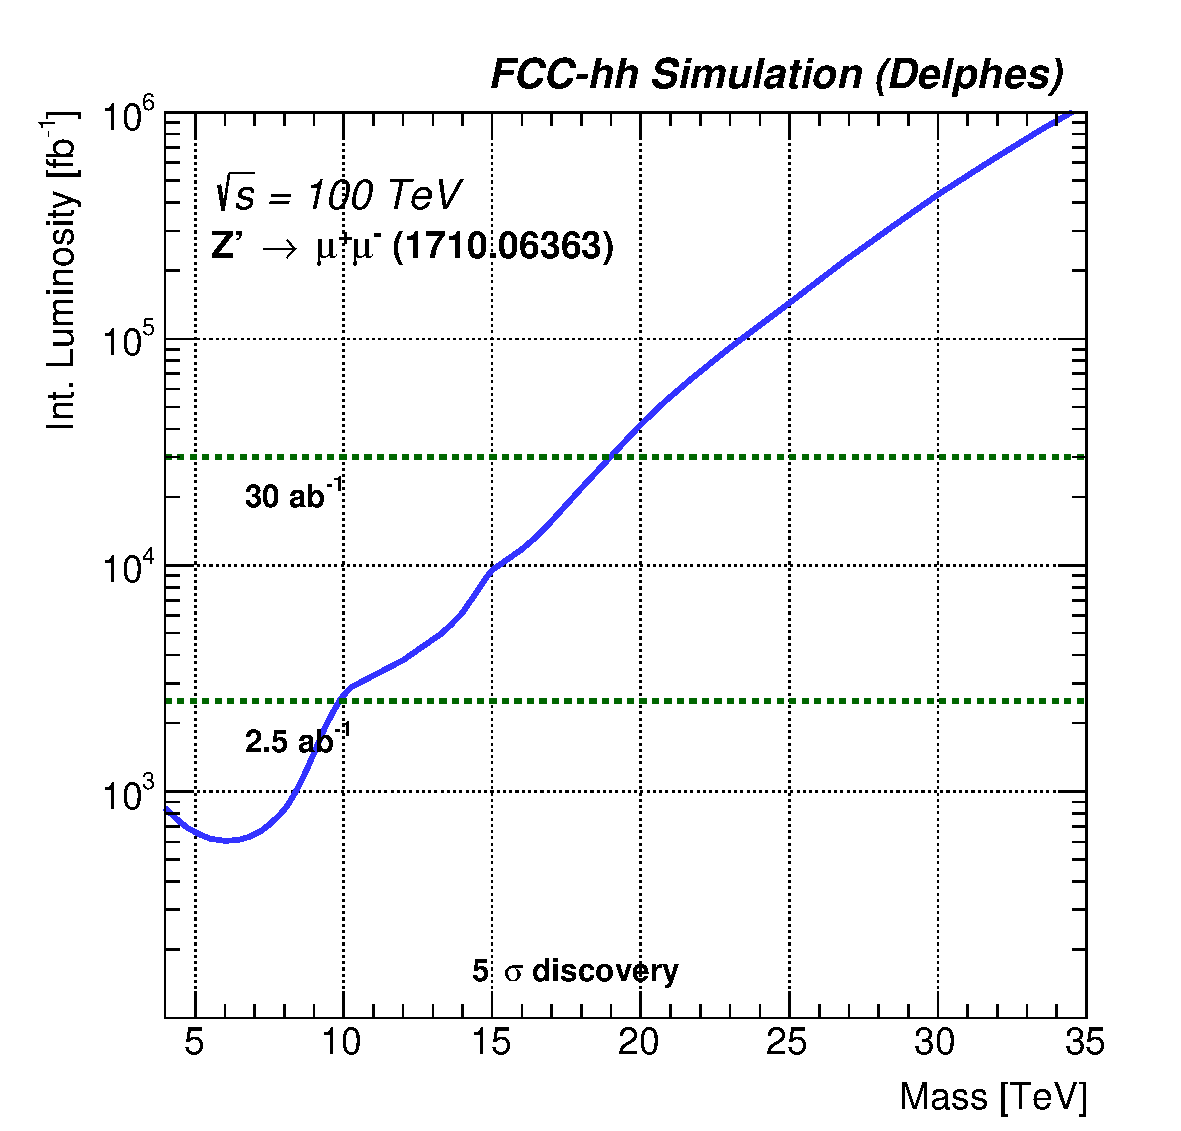
\includegraphics[width=0.32\columnwidth]{Fig/DiscoveryPotential_mumu_ano_rootStyle-eps-converted-to.pdf}
  \caption{Left : Invariant mass for a 30~TeV signal after full event selection in flavour anomaly scenario. Limit versus mass (middle) and luminosity for a $5\sigma$ discovery (right). }
  \label{figure:leptonicresonances:resultsmumu_flav}
\end{figure}

%%%%%%%%%%%%%%%%%%%%%%%%%%%%%%%%%%%%%%%%%%%%%%%%%%%%%
\section{Discussion on the detector performance}
\label{sec:detperf}

In the calorimeters, the energy resolution at high energy is determined by the constant term. The value of the constant term is different for ECAL and HCAL calorimeters. It is ultimately determined by the choice of the calorimeter technology and the design. Large constant term typically originate from inhomogenities among different detector elements and energy leakages due to sub-optimal shower containment. The calorimeters of the FCC-hh detector must therefore be capable of containing EM and hadronic showers in the multi-TeV regime in order to achieve small constant terms.
Compatibly with the LHC experiments, we require a performance of $\sigma_E/E~ \approx 0.3 \%$ and $\sigma_E/E~ \approx 3\%$ for the ECAL and HCAL respectively. As shown in Figure~\ref{figure:detperf} (left), the effect induced by the magnitude of the hadronic calorimeter constant term on the expected discovery reach for heavy \ZpSSM\ resonances decaying hadronically is sizable. We note that, despite the fraction of electromagnetic energy from $\pi^0$'s large in jets, the sensitivity is entirely driven by the hadronic calorimeter resolution given its worse intrinsic resolution.

Muons cannot be reconstructed with calorimetric methods~\footnote{~Calorimetric information can however help for muon identification. For example a 20\,TeV muon deposits through radiative energy loss on average $\Delta E=$~200 GeV in 3 meters of iron, corresponding to 1\% of the initial muon energy.}. Since the muon momentum is obtained through a fit of the trajectory that uses as input a combination of track and muon spectrometer hits, the muon momentum resolution resolution degrades with increasing momentum, as $\frac{\sigma_p}{p}= a \oplus b~p$ where $a$ is the constant term determined by the amount of material responsible for multiple scattering in the tracking volume. As with jets, electrons and photons, a good muon momentum resolution at multi-TeV energy is crucial for maintaining a high sensitivity in searches for heavy new states that might decay to muons. The reach for a \Zpmumu\ resonance obtained with various assumptions on the muon resolution is illustrated in Figure~\ref{figure:detperf} middle. The best sensitivity is achieved with an assumed $\sigma_p/p~ \approx 5\%$ at $p_T = 20$~TeV corresponding to our target for the FCC-hh detector, as opposed to the projected CMS resolution of $\sigma_p/p~\approx 40\%$. In order to reconstruct and measure accurately the momentum of $\pt=20~$TeV a large lever arm is needed and excellent spatial resolution and precise alignment of the tracking plus muon systems is needed. The specifics of design that allows to reach such required performance is discussed in the FCC CDR volume 3~\cite{cdr_volume3}.

New heavy states could decay to multi-TeV $c$ and $b$-quarks. FCC-hh detectors must therefore be capable of efficiently identifying multi-TeV long-lived hadrons. A $\pt=5$~TeV b-hadron is qualitatively very different from $\pt=100$~GeV b-hadron. The latter decays on average within the vertex detector acceptance and can be identified by means of displaced vertex reconstruction. Conversely, the former decays on average at a distance $\gamma c \tau = 50$~cm, well outside the pixel detector volume. Reconstructing such highly displaced b-jets will require a paradigm shit in heavy flavour reconstruction. The success of algorithms exploring large hit multiplicity discontinuities among sub-sequent tracking layer heavily relies on excellent granularity of the tracking system, in both longitudinal and transverse directions. High efficiencies ($\epsilon_b > 60\%$) for corresponding low mis-identification probability ($\epsilon_{u,d,s} < 1\%$) from light jets have to be achieved up to $\pt=5$~TeV. For example, searches for heavy resonances decaying to hadronic $\ttbar$ pairs heavily rely on efficient b-tagging performance at such energies. The discovery reach for a specific $Z'$ model assuming several scenarios for b-jet identification at high energies is shown in Figure~\ref{figure:detperf} right. Various scenarios of b-tagging efficiencies at very large \pt\ are considered. The nominal efficiency is given in Table~\ref{tab:effs}, and scenarii 1,2 and 3 correspond to reduction of the slope respectively by a factor 25\%, 33\% and 50\%. As expected the discovery reach strongly depends on the b-tagging performances.

\begin{figure}[!htb]
  \centering
    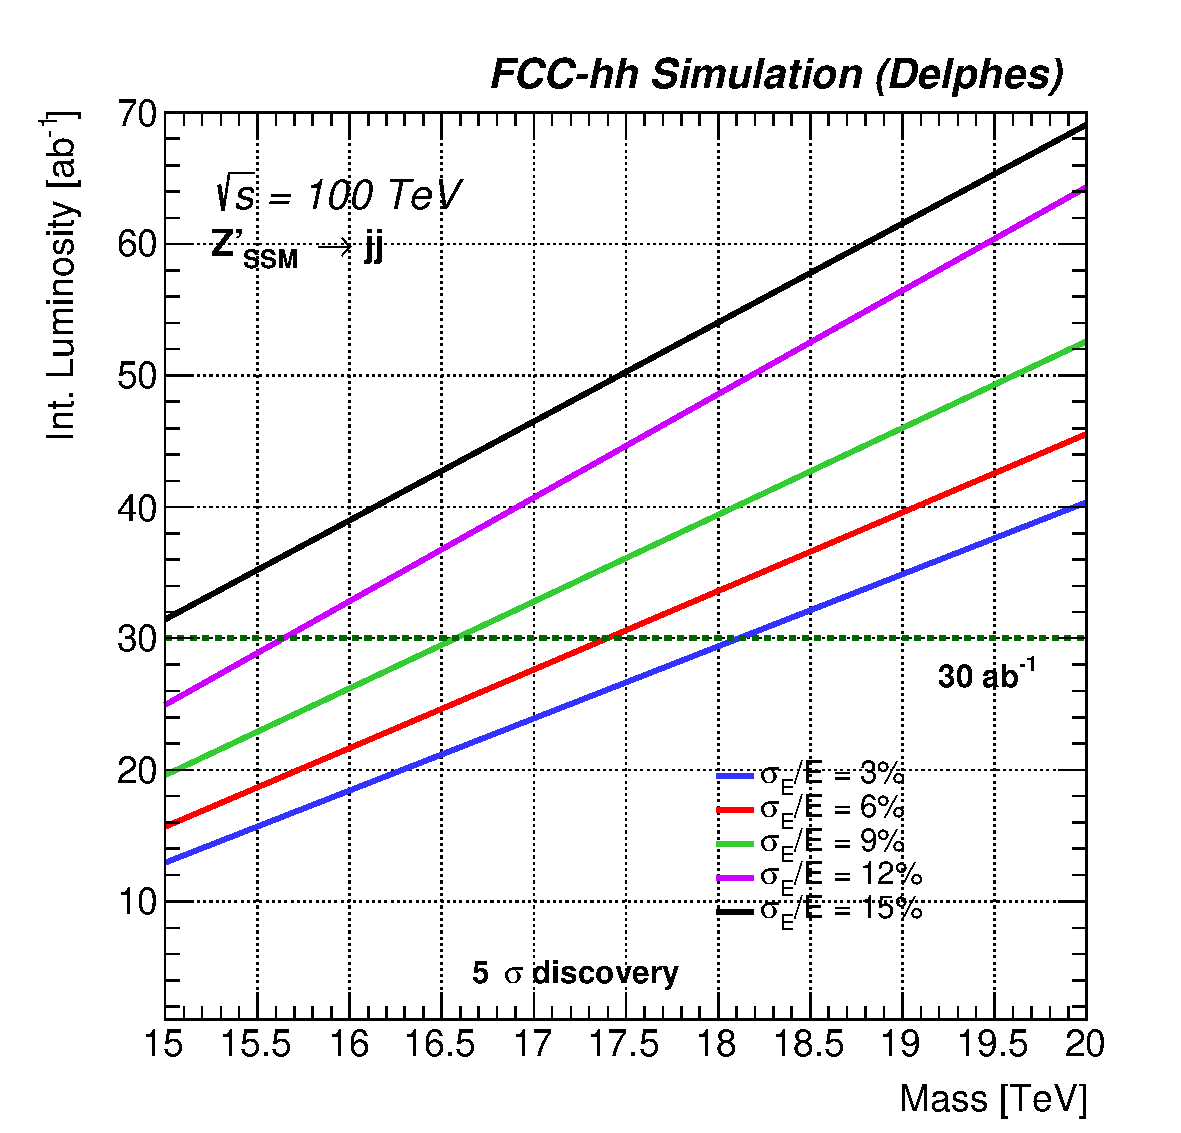
\includegraphics[width=0.32\columnwidth]{Fig/DiscoveryPotential_Zp_jj_comb_smeared_rootStyle-eps-converted-to.pdf}
  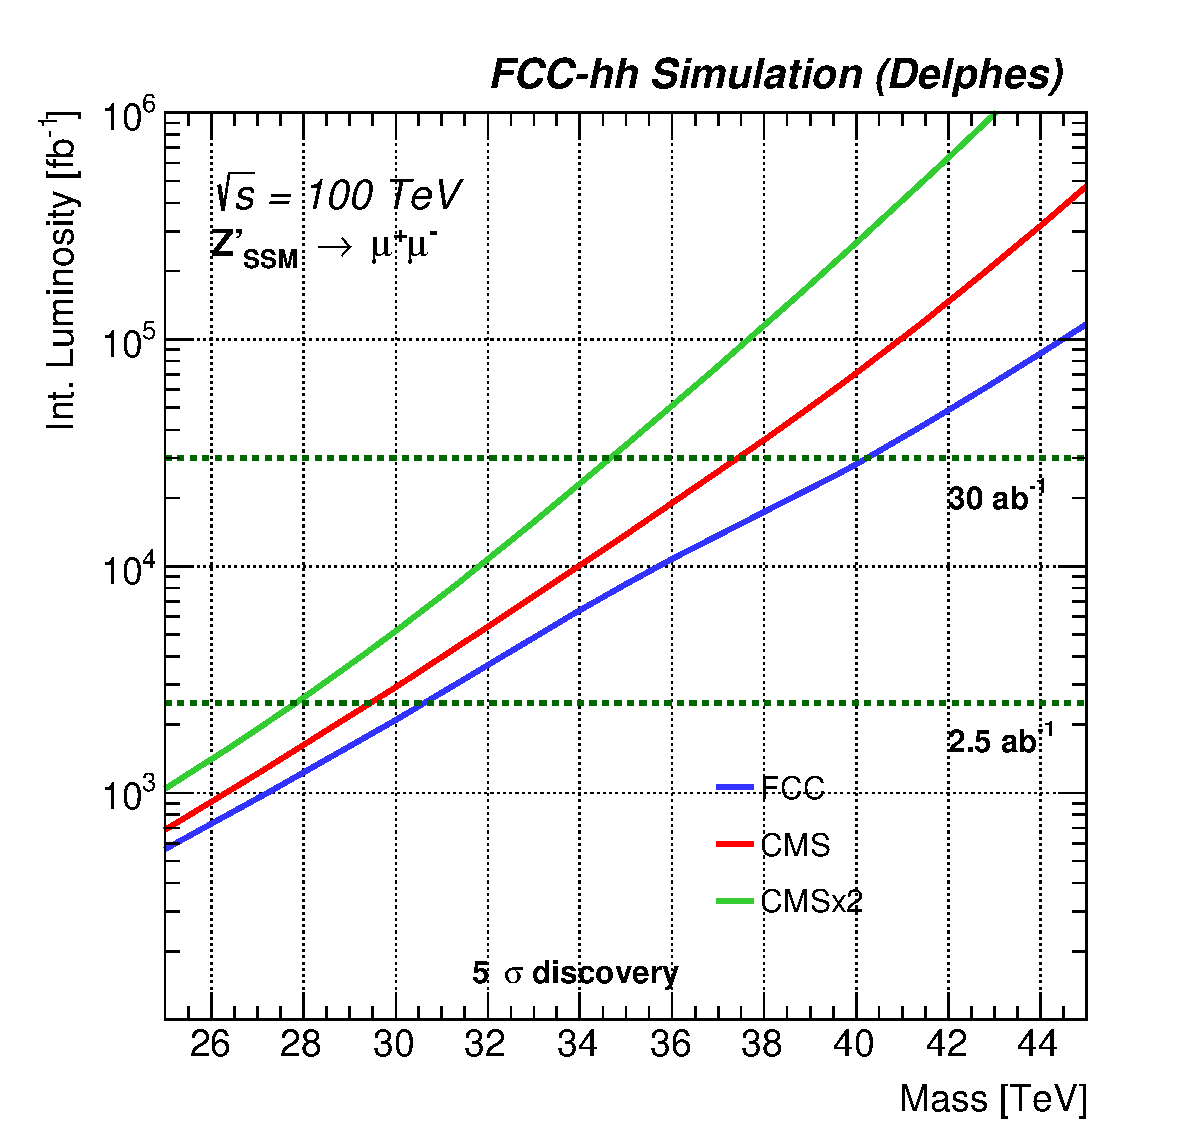
\includegraphics[width=0.32\columnwidth]{Fig/DiscoveryPotential_ll_smearhl_rootStyle-eps-converted-to.pdf}
  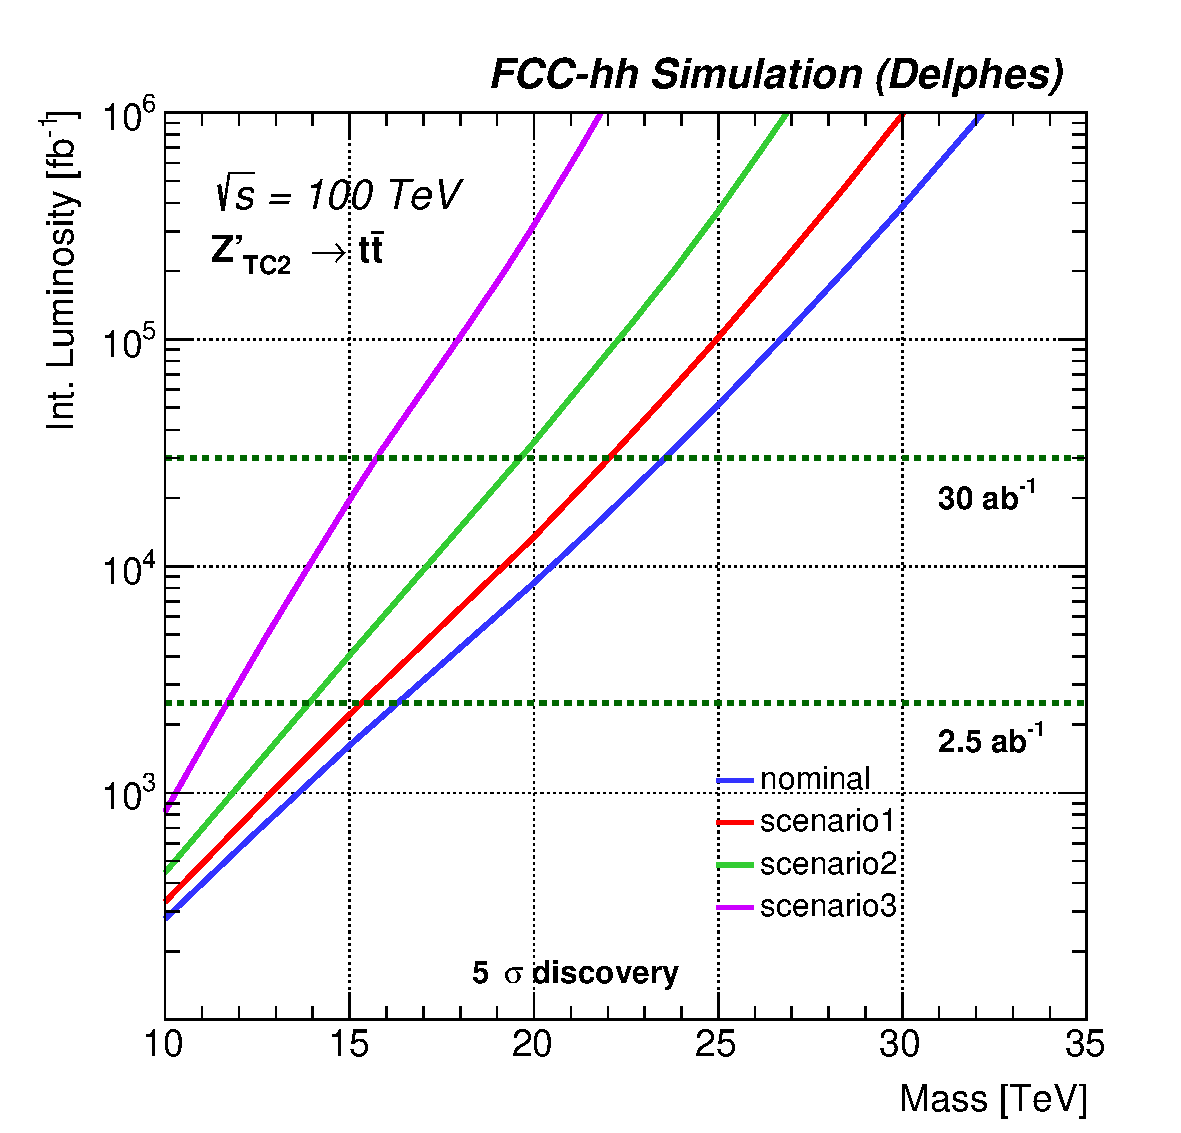
\includegraphics[width=0.32\columnwidth]{Fig/DiscoveryPotential_tt_TC2_tagger_TRFbtag_degrade_rootStyle-eps-converted-to.pdf}
  \caption{Left : Invariant mass for a 30~TeV signal after full event selection in flavour anomaly scenario. Limit versus mass (middle) and luminosity for a $5\sigma$ discovery (right). }
  \label{figure:detperf}
\end{figure}



%%%%%%%%%%%%%%%%%%%%%%%%%%%%%%%%%%%%%%%%%%%%%%%%%%%%%
\section{Conclusion}
\label{sec:conc}

This paper presents studies of a search for heavy resonances decaying to leptons, bosons, top or light quarks in the context of energy frontier colliders. 

\appendix
%%%%%%%%%%%%%%%%%%%%%%%%%%%%%%%%%%%%%%%%%%%%%%%%%%%%%
\section{Multivariate object tagger}%appendix
\label{sec:app:mva}
The training samples are built from jets that do not contain leptons, that could come from semi-leptonic b-decays. As an example, the $E_{F}(n=1,\alpha=0.05)$ observable used in the $W$-tagger is shown in Figure~\ref{fig:TMVA_final_result} left and the $\tau_{32}$ observable used in the top-tagger is on the right. The evolution of the light jet efficiency versus the $W$ and top tagging efficiencies for both taggers is shown in Figure~\ref{fig:TMVA_final_result} right. Cross-checks have been performed to further validate the multivariate procedure. First, by removing highly correlated variables the same performances are achieved. Second, the BDT response has been tested for different signal masses to understand how the mass dependence could affect the analyses. For the cut used in the analysis (BDT score greater than 0.15), the shape of the BDT is not dramatically changing the signal efficiency. The input variables used to train the BDT, ordered by training weight, can be found in table~\ref{tab:TMVA_summary}.

\begin{table}[!htb]\centering
\begin{tabular}{| l | c | l | c |}
\hline
  \multicolumn{2}{|c|}{$W$ tagger}  & \multicolumn{2}{c|}{top tagger} \\
  \hline
 variable & weight & variable & weight \\
\hline
% rename them
 $\tau_3$ (track jet, R=0.2)      & 0.12      & $\tau_1$ (track jet, R=0.2) & 0.21  \\
 $\mSD$  (track jet, R=0.2)      & 0.11      & $\mSD$  (track jet, R=0.2) & 0.17 \\
 $\tau_{31}$  (track jet, R=0.2) & 0.10     & $\tau_{31}$  (track jet, R=0.2)  & 0.11 \\
 $E_{F}(n=5,\alpha=0.05)$                               & 0.09     &  $\tau_2$ (track jet, R=0.2) & 0.10 \\
 $E_{F}(n=4,\alpha=0.05)$                               & 0.09     & $\tau_3$ (track jet, R=0.2) & 0.09 \\
 $E_{F}(n=1,\alpha=0.05)$                               & 0.08     & $\mSD$  (track jet, R=0.8)& 0.09 \\
 $E_{F}(n=2,\alpha=0.05)$                               & 0.07     &  $\mSD$  (track jet, R=0.4) & 0.09 \\
 $E_{F}(n=3,\alpha=0.05)$                               & 0.06     & $\tau_{32}$  (track jet, R=0.2) & 0.08 \\
 $\tau_{21}$  (track jet, R=0.2)& 0.06   & $\tau_{21}$  (track jet, R=0.2) & 0.06 \\
 $\mSD$  (track jet, R=0.8) & 0.06 &  &\\
 $\mSD$  (track jet, R=0.4) & 0.06 & & \\
 $\tau_1$ (track jet, R=0.2) & 0.05      &  &\\
 $\tau_2$ (track jet, R=0.2) & 0.04      &  &\\
 $\tau_{32}$  (track jet, R=0.2) & 0.02    &  &\\
\hline
\end{tabular}
\caption{Summary of the input variables to the BDT and their relative weight for both $W$ and top taggers. \CH{could drop that table}}
\label{tab:TMVA_summary}
\end{table}



\begin{figure}[!htbp]\centering
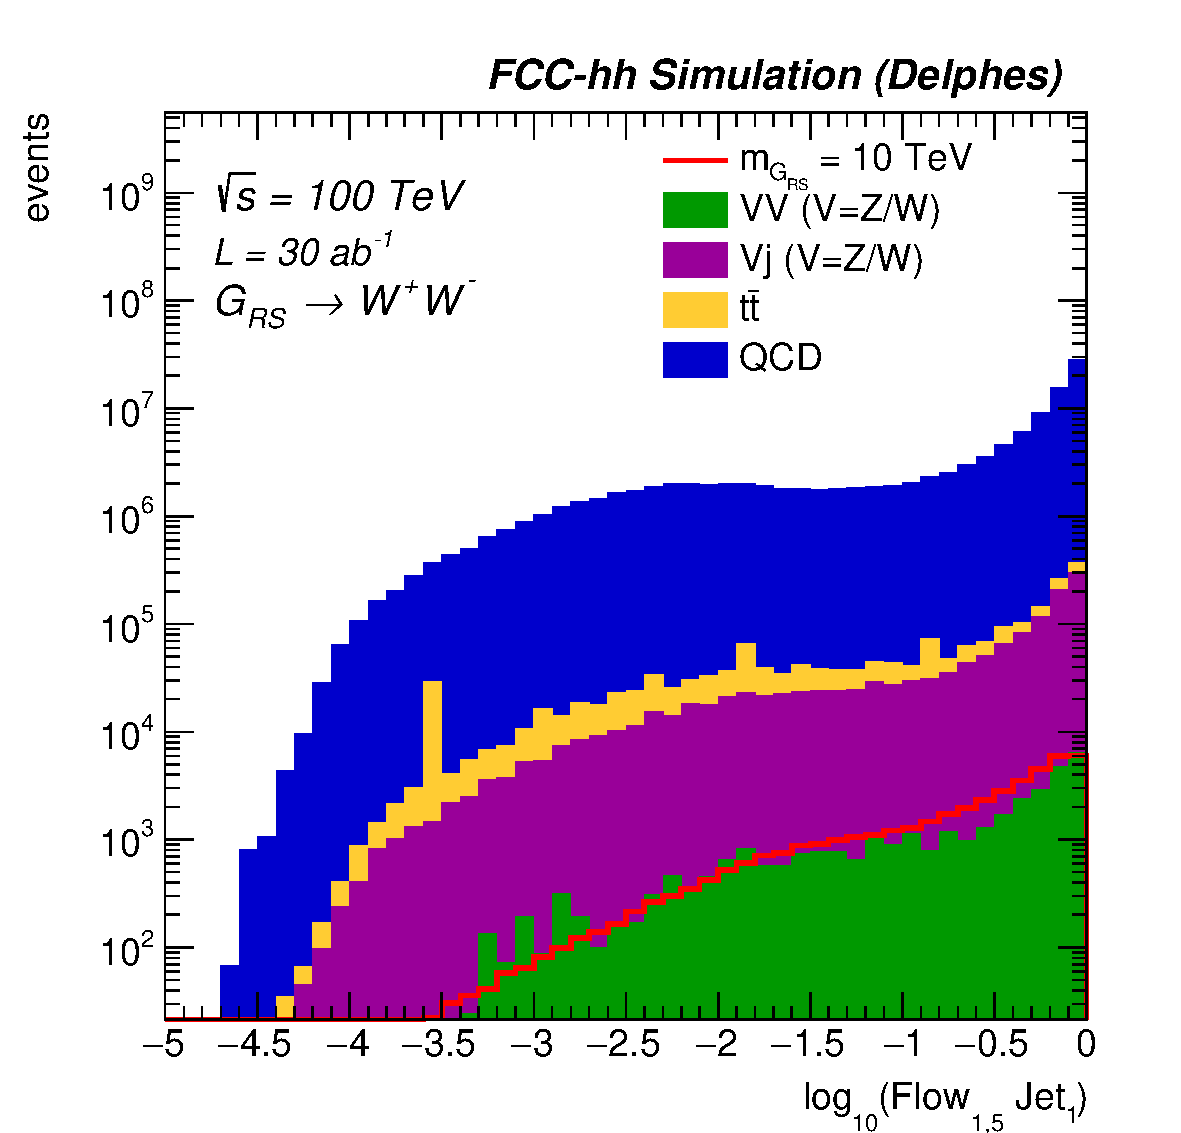
\includegraphics[width=0.32\textwidth]{Fig/TMVA/Jet1_Flow15_sel0_nostack_logx-eps-converted-to.pdf}
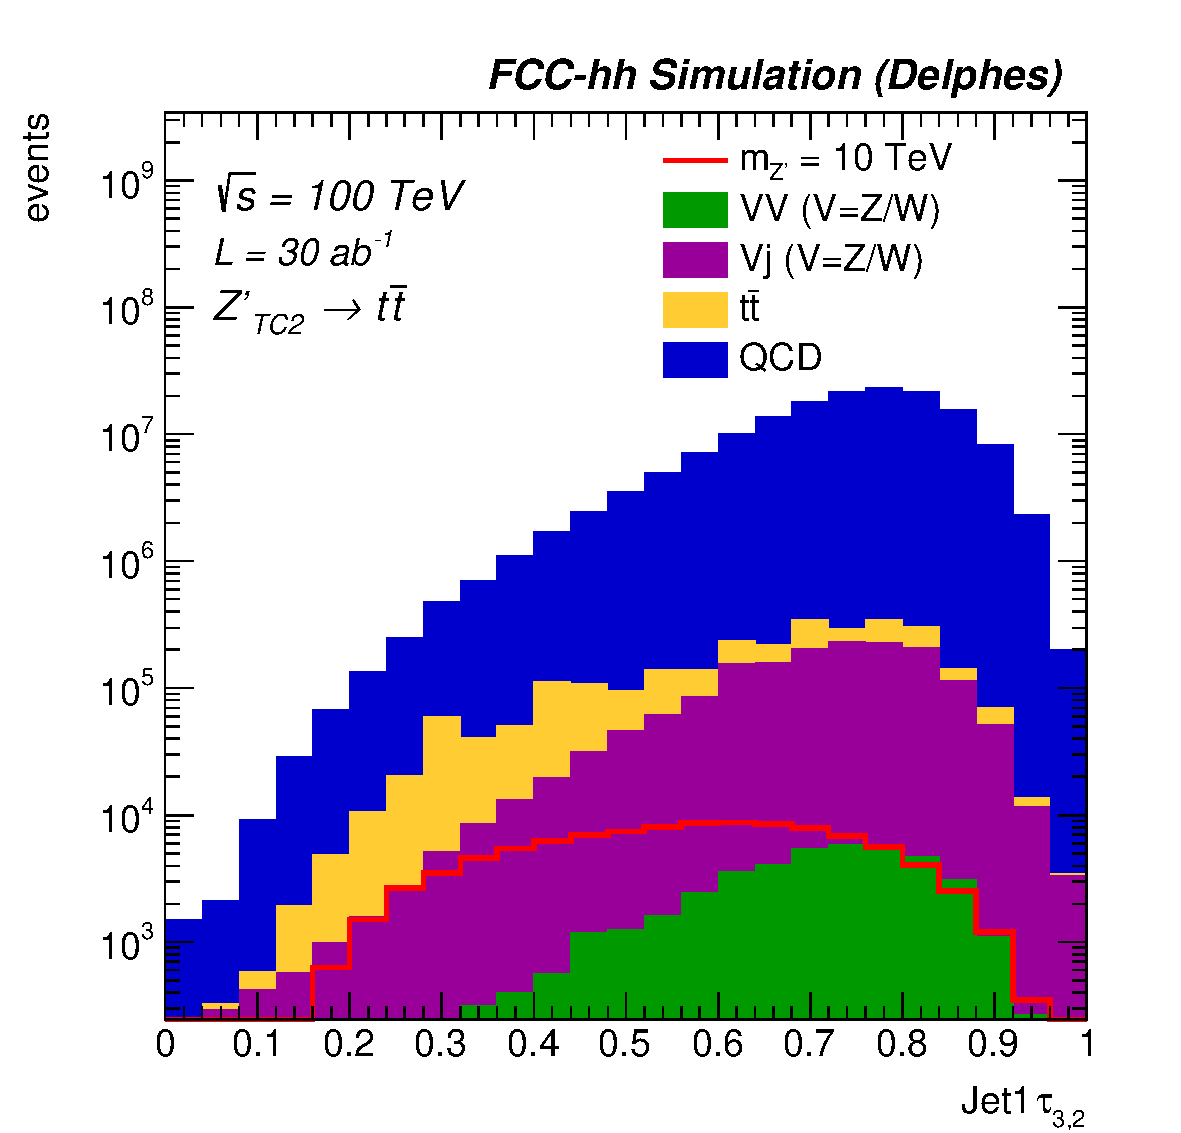
\includegraphics[width=0.32\textwidth]{Fig/TMVA/Jet1_tau32_sel0_nostack_log-eps-converted-to.pdf}
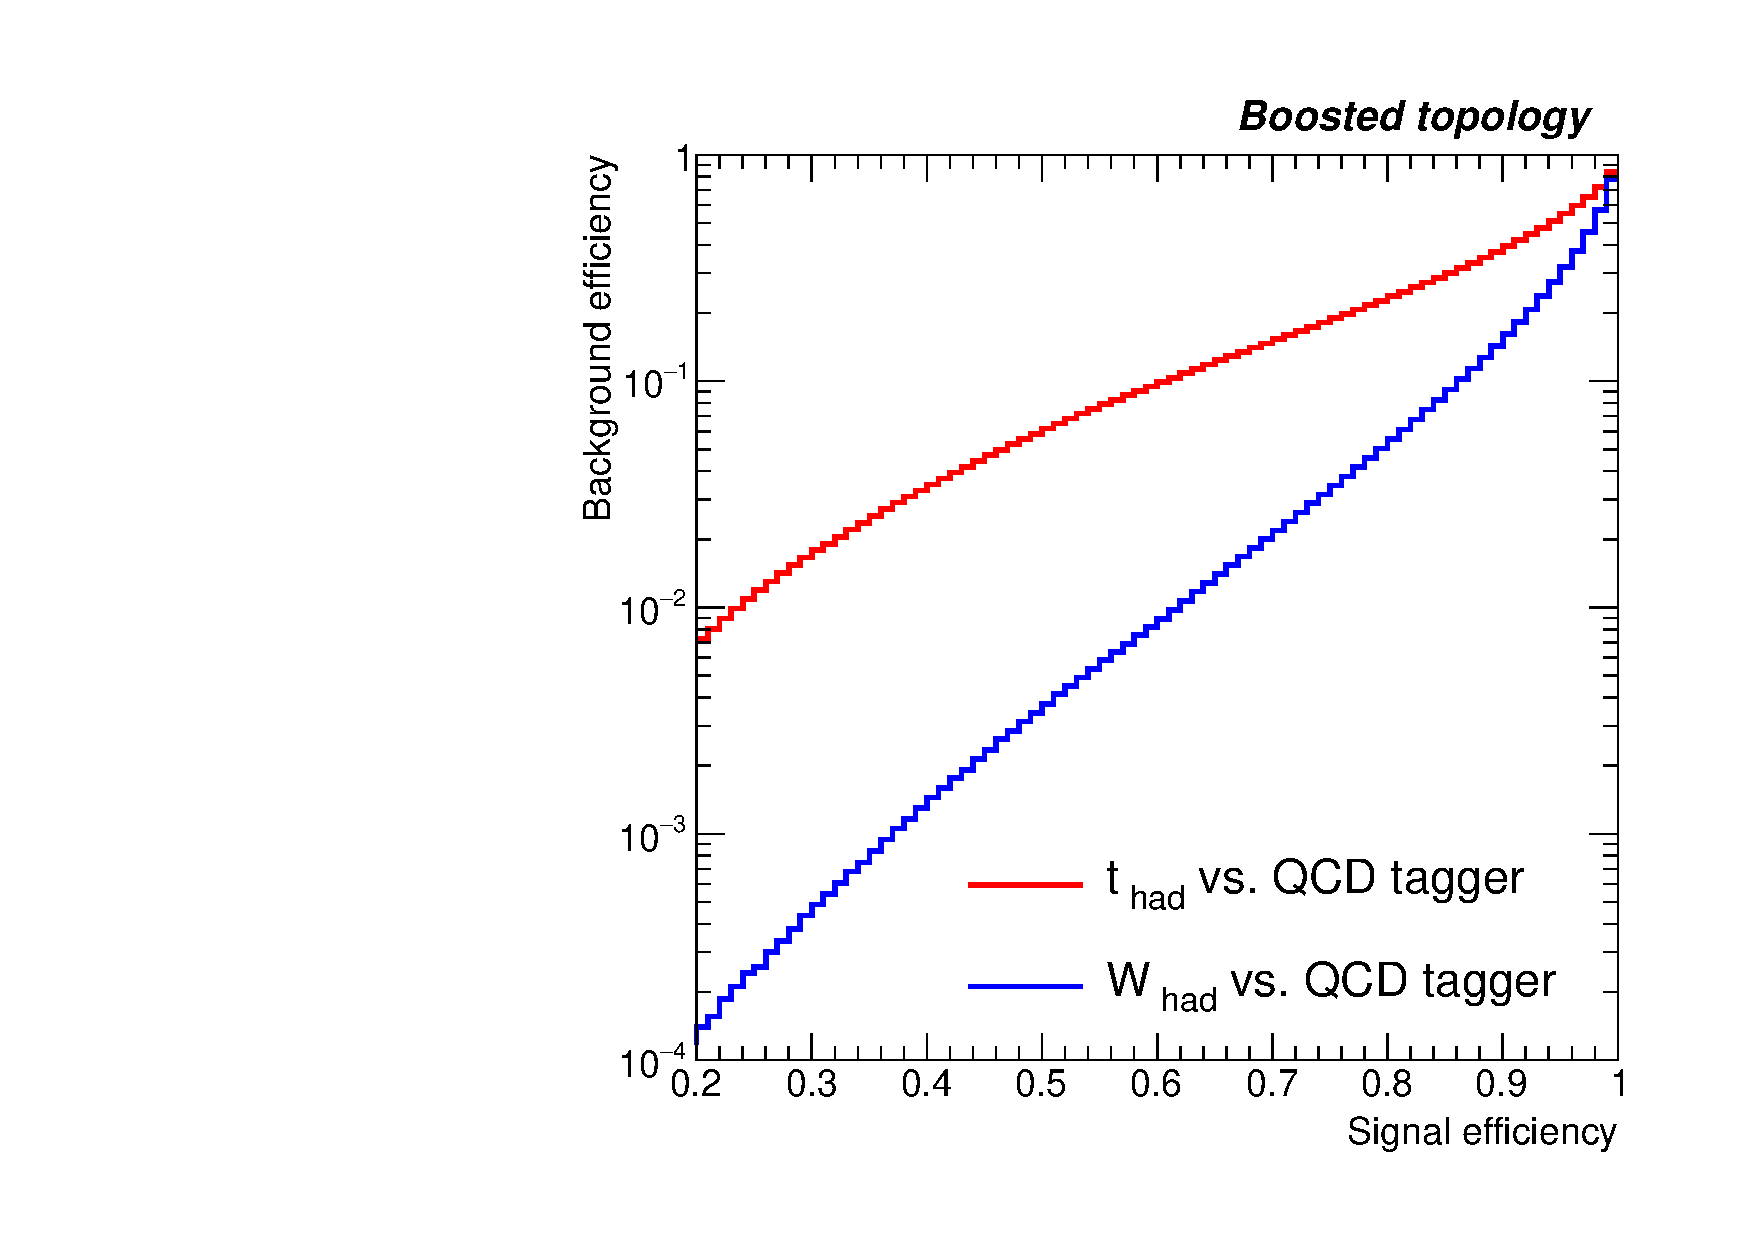
\includegraphics[width=0.32\textwidth]{Fig/TMVA/effQCD_vs_effWhadBlue_thadRed_log.pdf}
\caption{Left: Energy-flow $E_{F}(n=1,\alpha=0.05)$ observable for the leading jet $p_T$ of the \rsg\ analysis at the pre-selection level (two high $p_T$ jets). Middle: $\tau_{32}$ observable for the leading jet $p_T$ of the \Zptt\ analysis at the pre-selection level (two high $p_T$ jets). Right: Light jet rejection versus tagging efficiency for the $W$-tagger (blue) and top-tagger (red)}
\label{fig:TMVA_final_result}
\end{figure}


%%%%%%%%%%%%%%%%%%%%%%%%%%%%%%%%%%%%%%%%%%%%%%%%%%%%%
\section{Tagging rate function}%appendix
\label{sec:app:trf}
Given a jet with $\eta$, $\pt$ and flavour $f$, its tagging probability can be noted as:
\begin{equation*}
	\varepsilon \left(f,|\eta|,\pt\right)
\end{equation*}
\newline
For a given event with $N$ jets, its probability of containing exactly one $b$-tag jet can be computed as:
\begin{equation*}
	P_{=1} = \sum\limits_{i=1}^N \left( \varepsilon_{i} \prod\limits_{i \neq j} \left( 1 - \varepsilon_{j} \right) \right)
\end{equation*}
\newline
In the same way, it can be used to compute the probability for inclusive $b$-tag selections:
\begin{align*}
	P_{=0} &= \prod\limits_{i=1}^N \left( 1 - \varepsilon_{j} \right) \\
	P_{\geq 1} &= 1 - P_{=0}
\end{align*}
\newline
It was verify that the TRF methods agrees well with the direct tagging.


%%%%%%%%%%%%%%%%%%%%%%%%%%%%%%%%%%%%%%%%%%%%%%%%%%%%%
\section{Background fit}%appendix
\label{sec:app:bgfit}
The function used to fit the background shapes when Monte-Carlo statistic is insufficient can be expressed as:
\begin{equation}
\label{eq:fitfunc}
f(z)=p_1(1-z)^{p_2}z^{p_3}z^{p_{4}logz}
\end{equation}
where $z=m_{jj}/\sqrt{s}$, with $m_{jj}$ the invariant mass of the two high energetic objects and $\sqrt{s}$ the center of mass energy. Fitting the invariant mass distribution with the function~\ref{eq:fitfunc} allows to obtain a smooth shape, while the overall normalisation is taken prior to the fit. Figure~\ref{fig:hadronicresonances_nofit}) left shows the \Zptt\ invariant mass distribution after the final selection for the various backgrounds and a 10\,TeV signal. Large statistical fluctuations can be observed especially for the QCD background that is heavily suppressed thanks to the multivariate object tagger. The right plot represents the same QCD invariant mass distribution before the fit (dots) and after the fit (plain). Good agreement is observed and the fitted distribution normalised to the pre-fit yields is used to obtain the results in the statistical analysis.

\begin{figure}[!htb]\centering
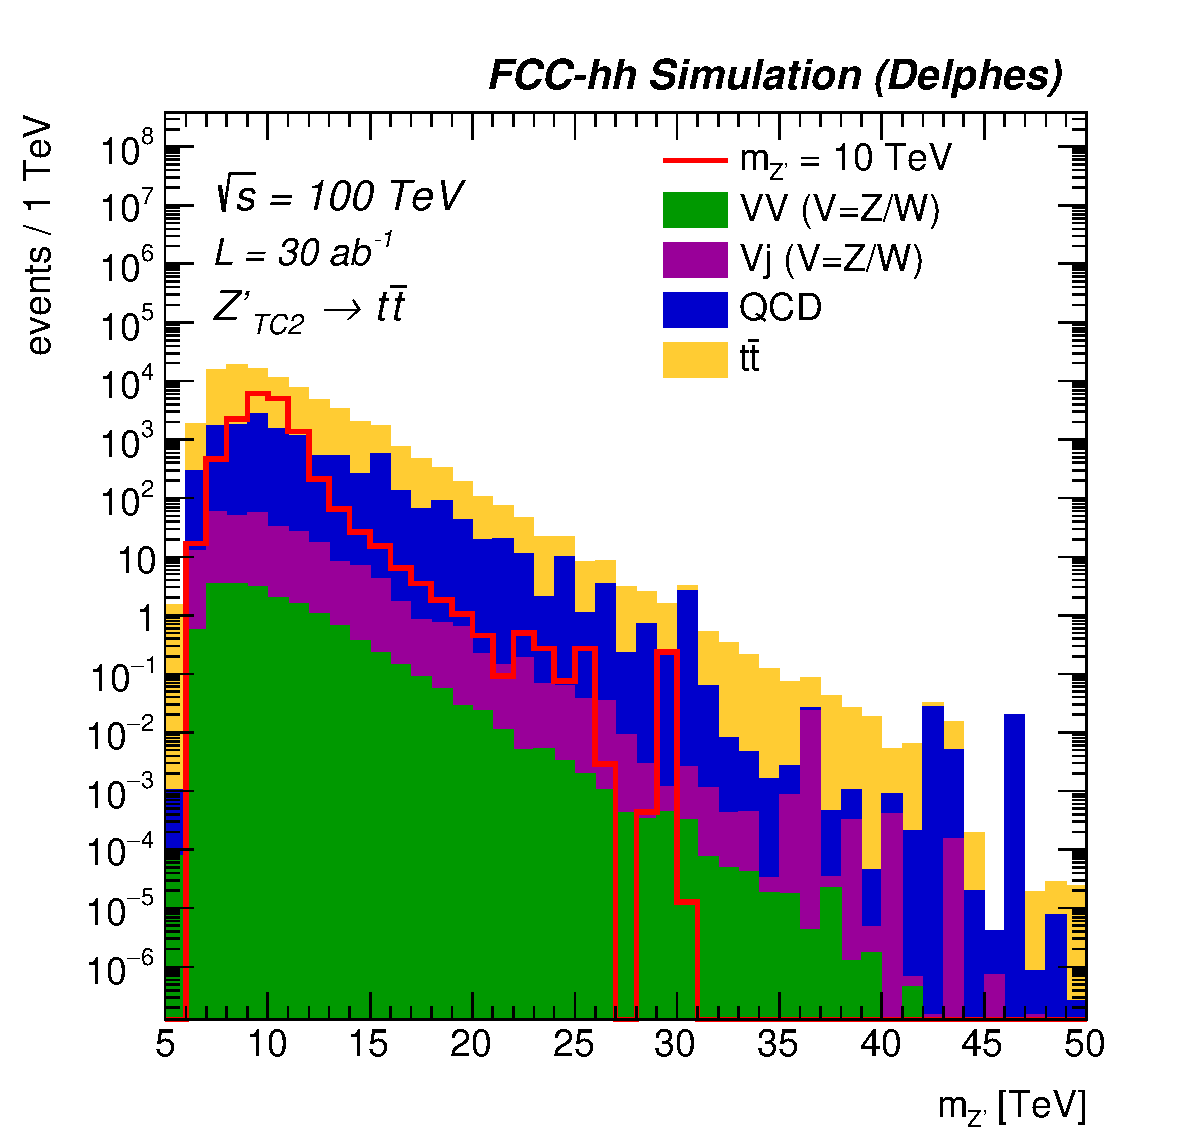
\includegraphics[width=0.49\columnwidth]{Fig/Zptt/Mj1j2_pf08_MetCorr_sel8_nostack_log-eps-converted-to.pdf}
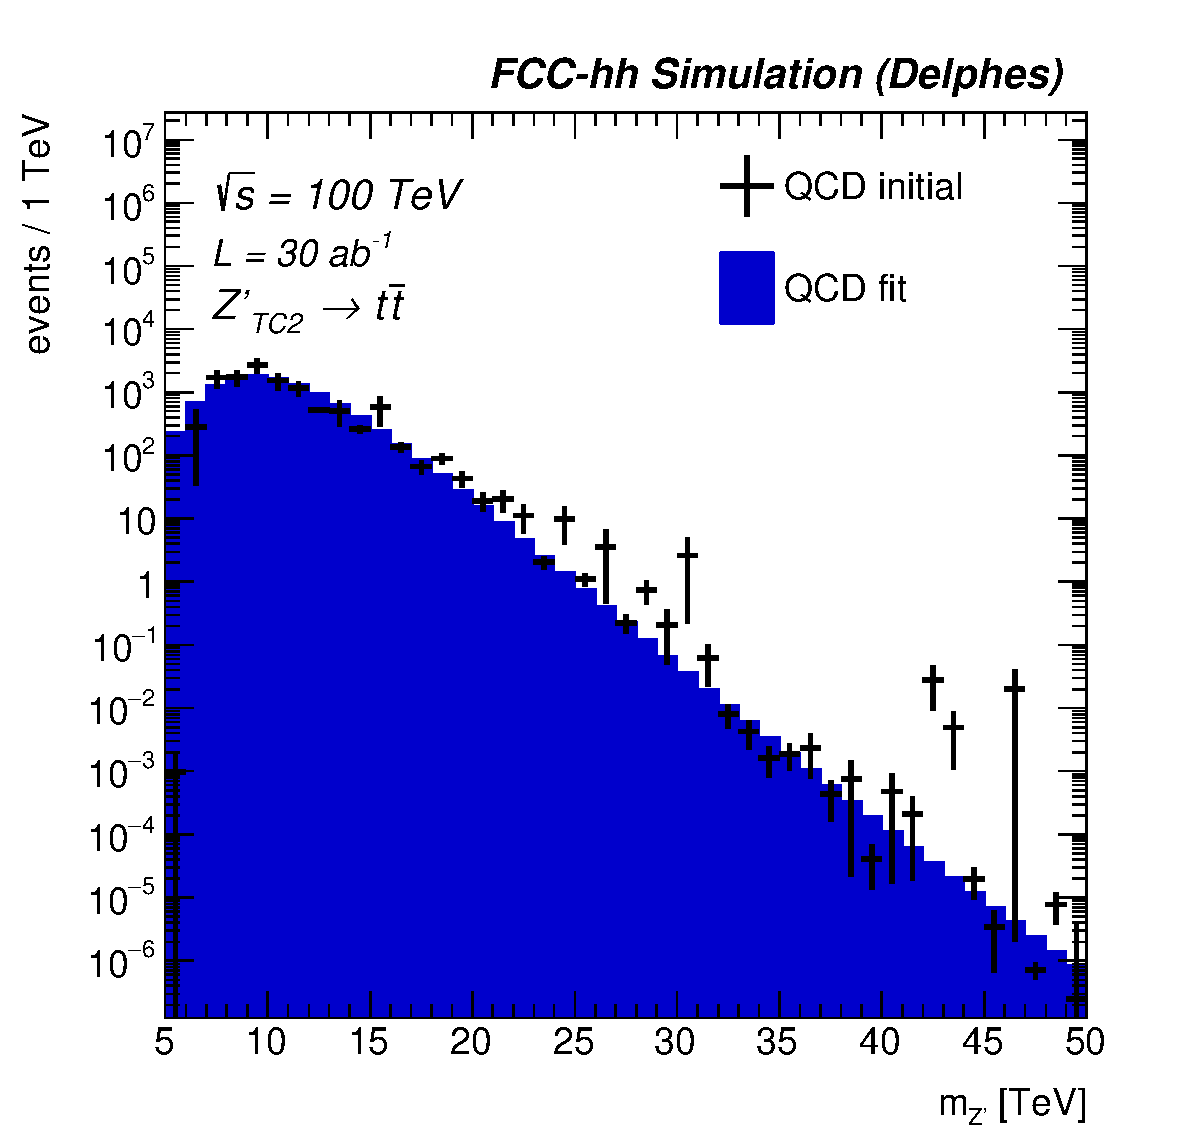
\includegraphics[width=0.49\columnwidth]{Fig/Zptt/Zptt_QCD_sel8_Mj1j2_pf08_MetCorr_fit-eps-converted-to.pdf}
\caption{Invariant mass prior to fit.}
\label{fig:hadronicresonances_nofit}
\end{figure}



%%%%%%%%%%%%%%%%%%%%%%%%%%%%%%%%%%%%%%%%%%%%%%%%%%%%%%appendix%appendix
\section{Summary plots}
The discovery potential (top) and 95\% CL limits (bottom) for the heavy resonances presented in this document are summarised in Figure~\ref{figure:resonances100:summary} for FCC-hh (left) and HE-LHC (right).
\begin{figure}[!htb]
  \centering
  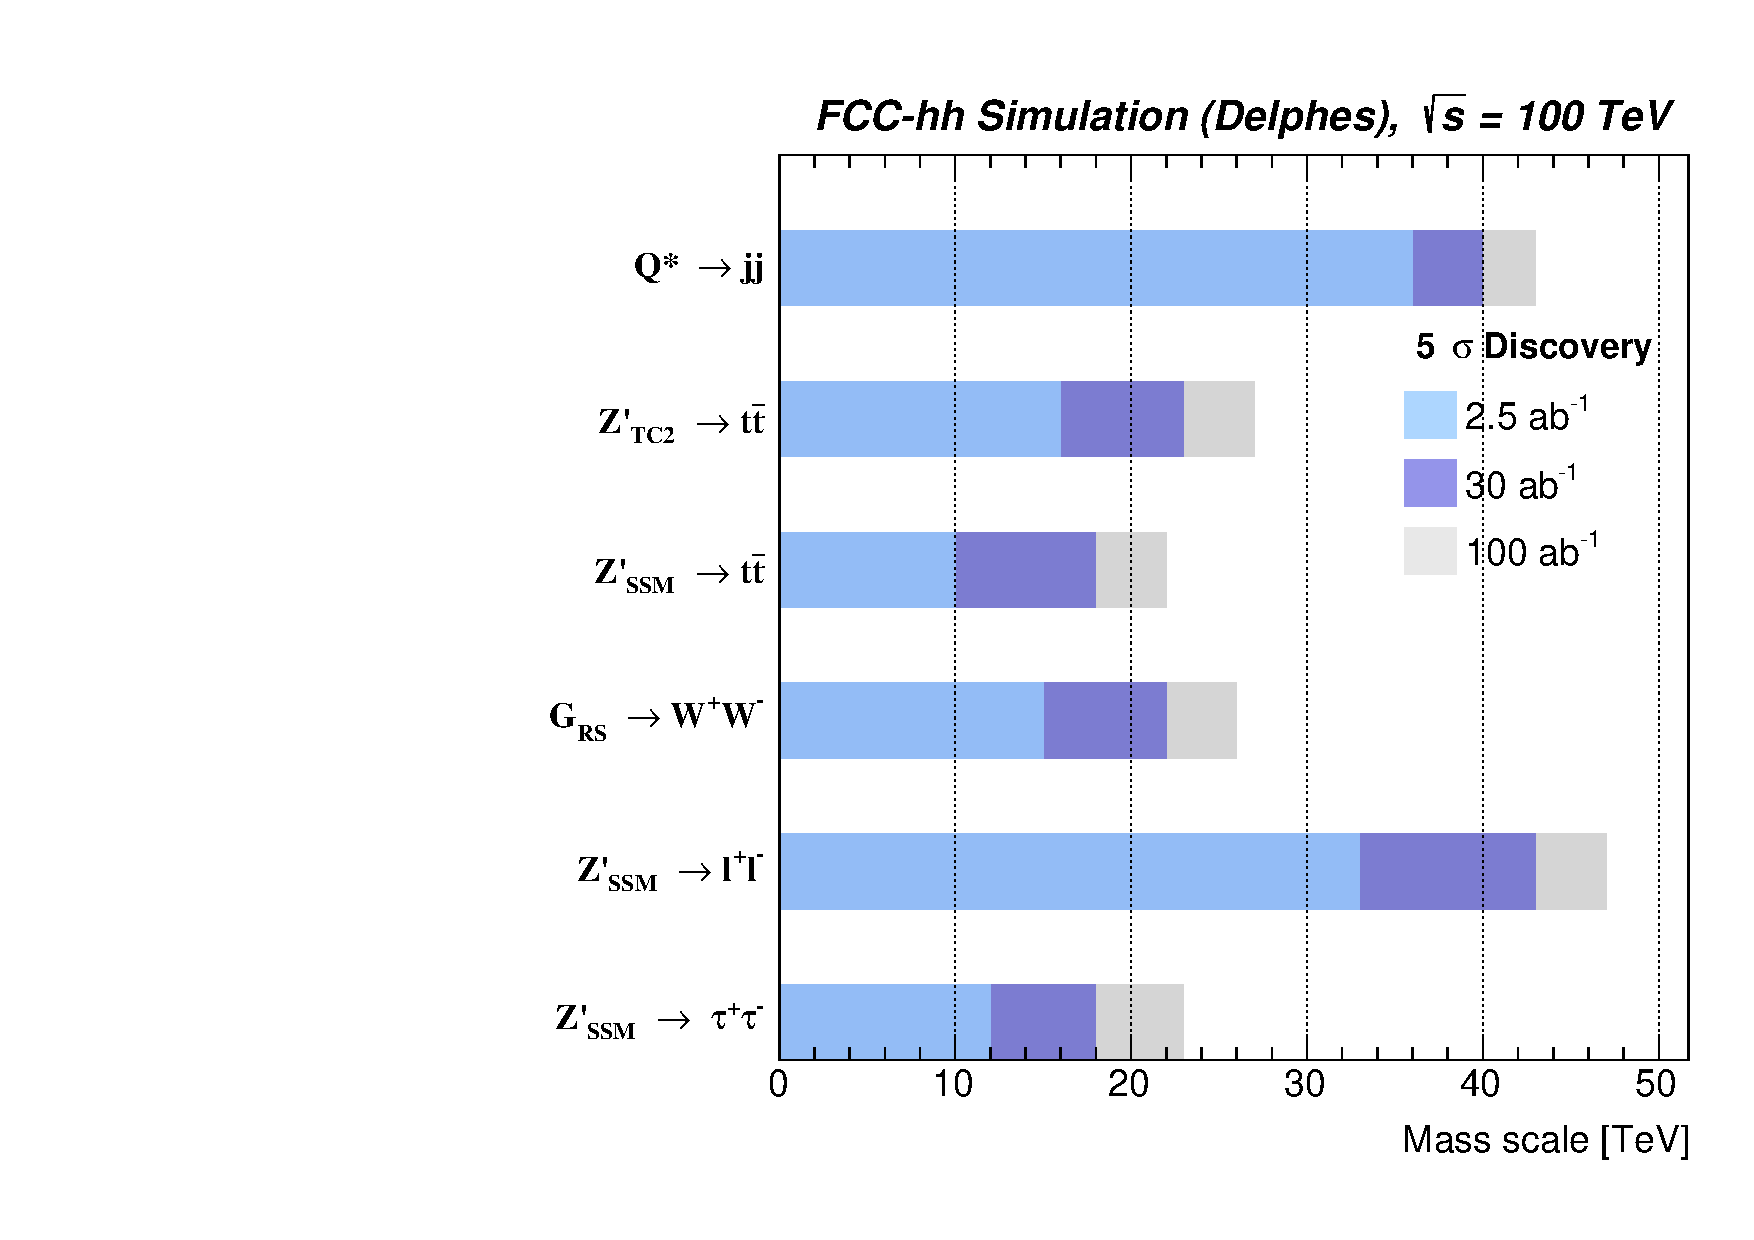
\includegraphics[width=0.49\columnwidth]{Fig/summaryDisco_onlyFCChh.pdf}
  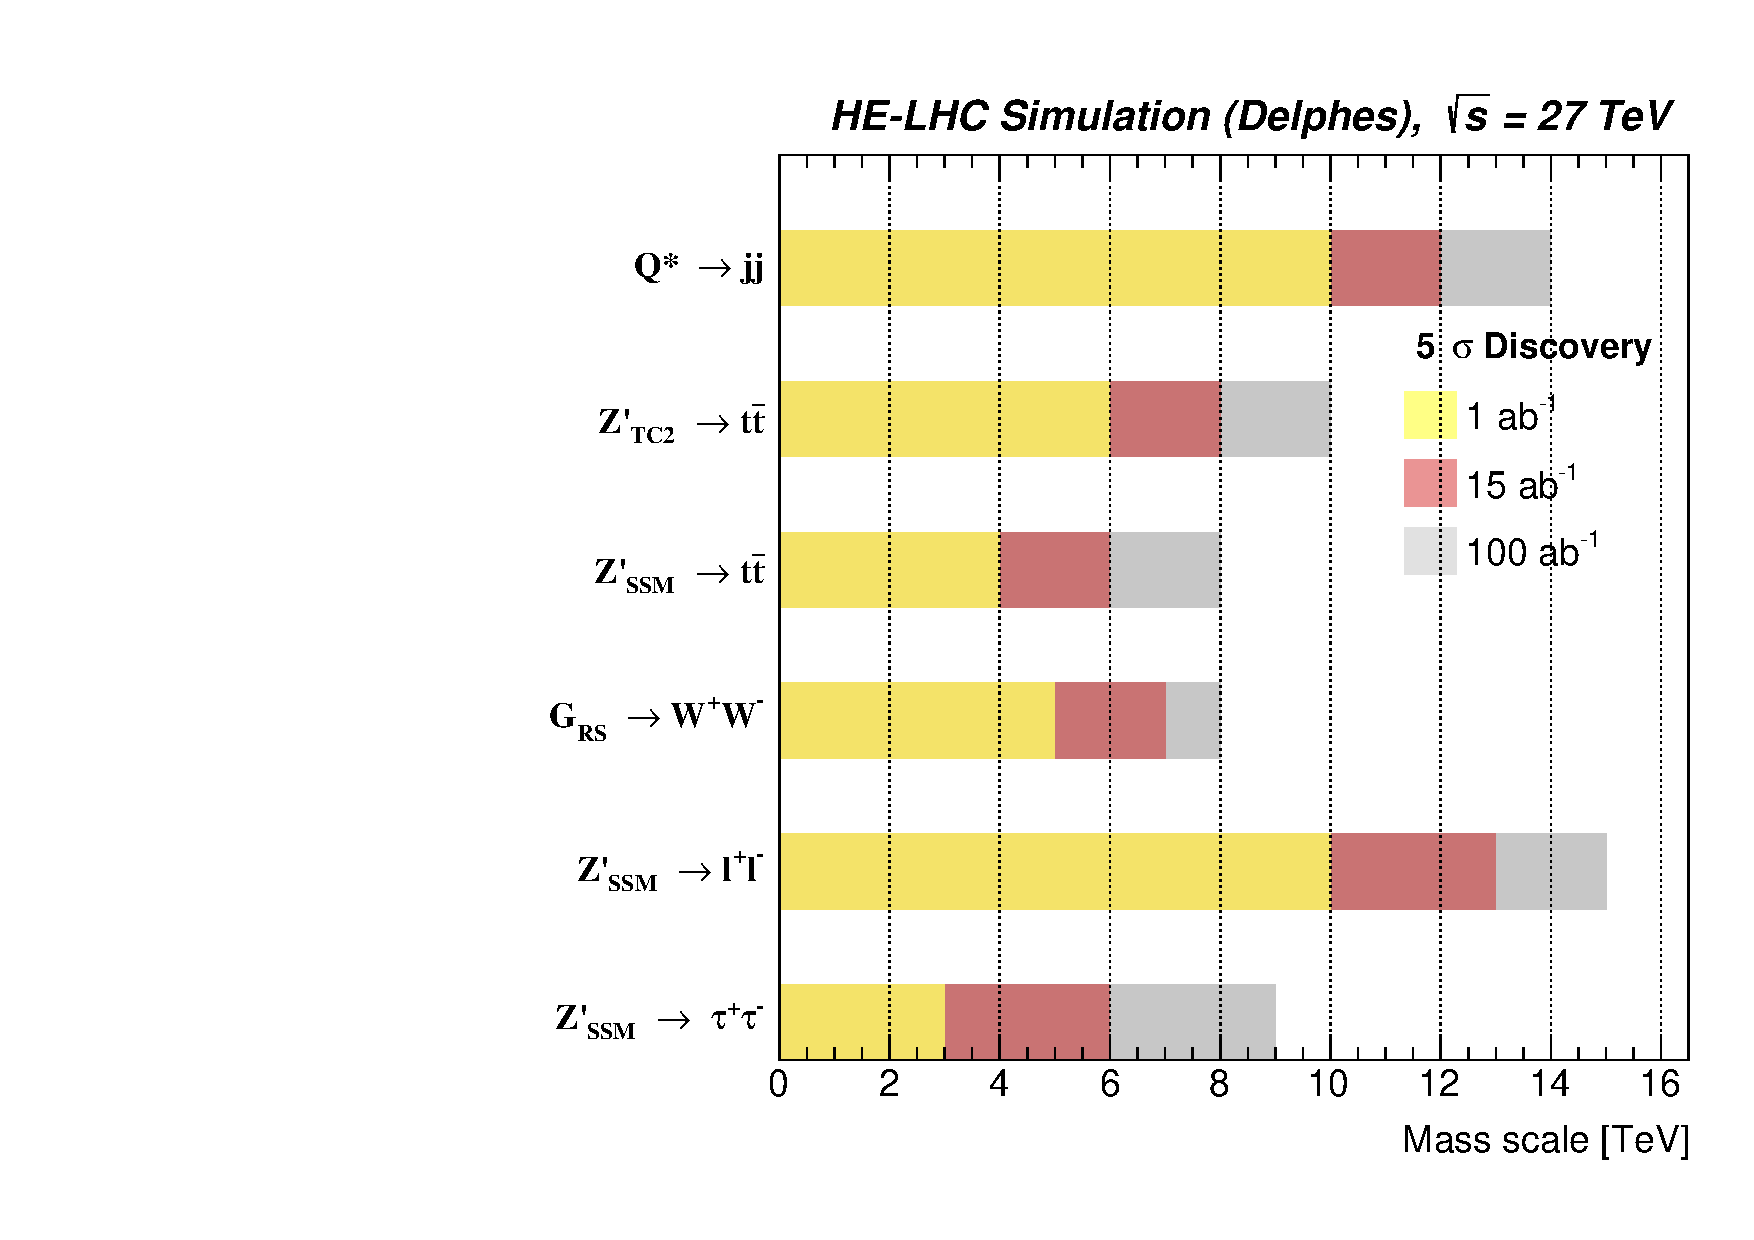
\includegraphics[width=0.49\columnwidth]{Fig/summaryDisco_onlyHELHC.pdf}
   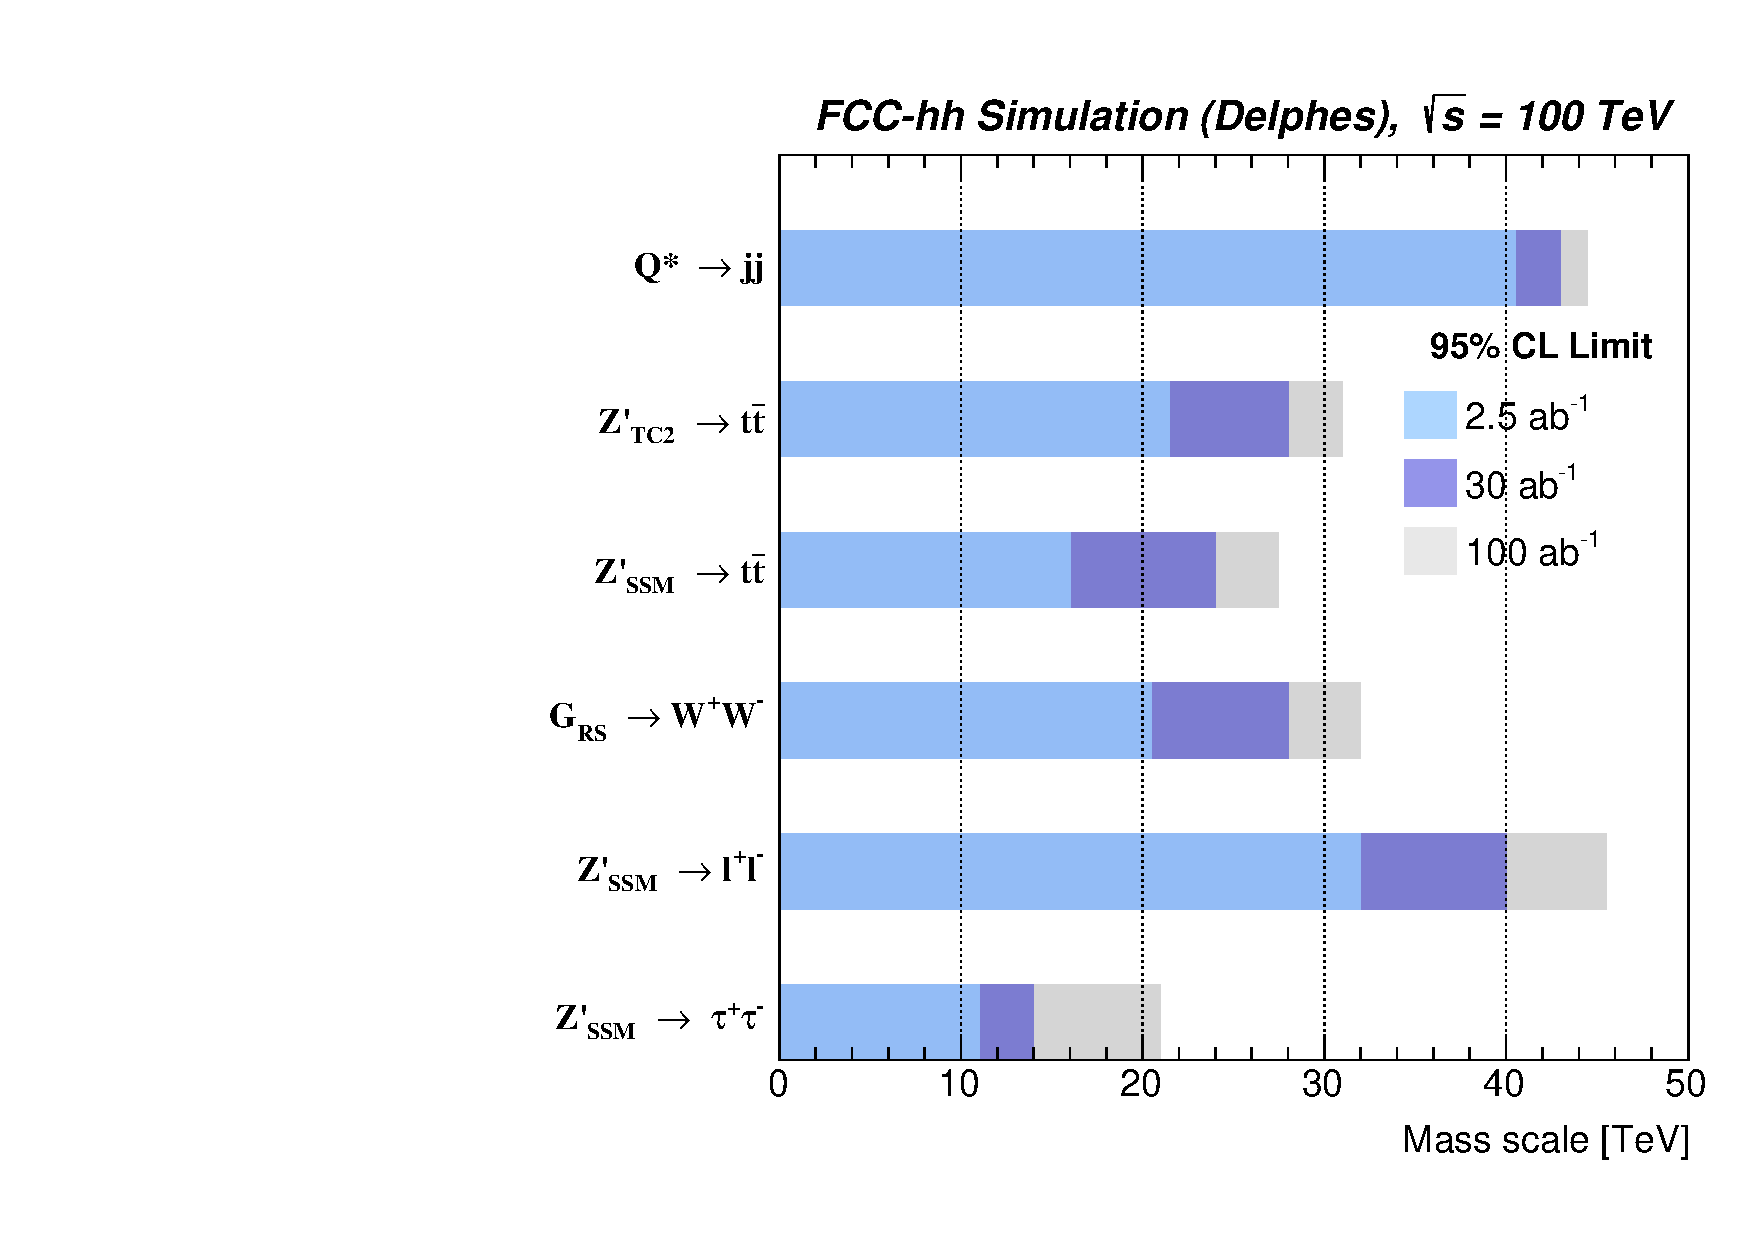
\includegraphics[width=0.49\columnwidth]{Fig/summaryLimit_onlyFCChh.pdf}
  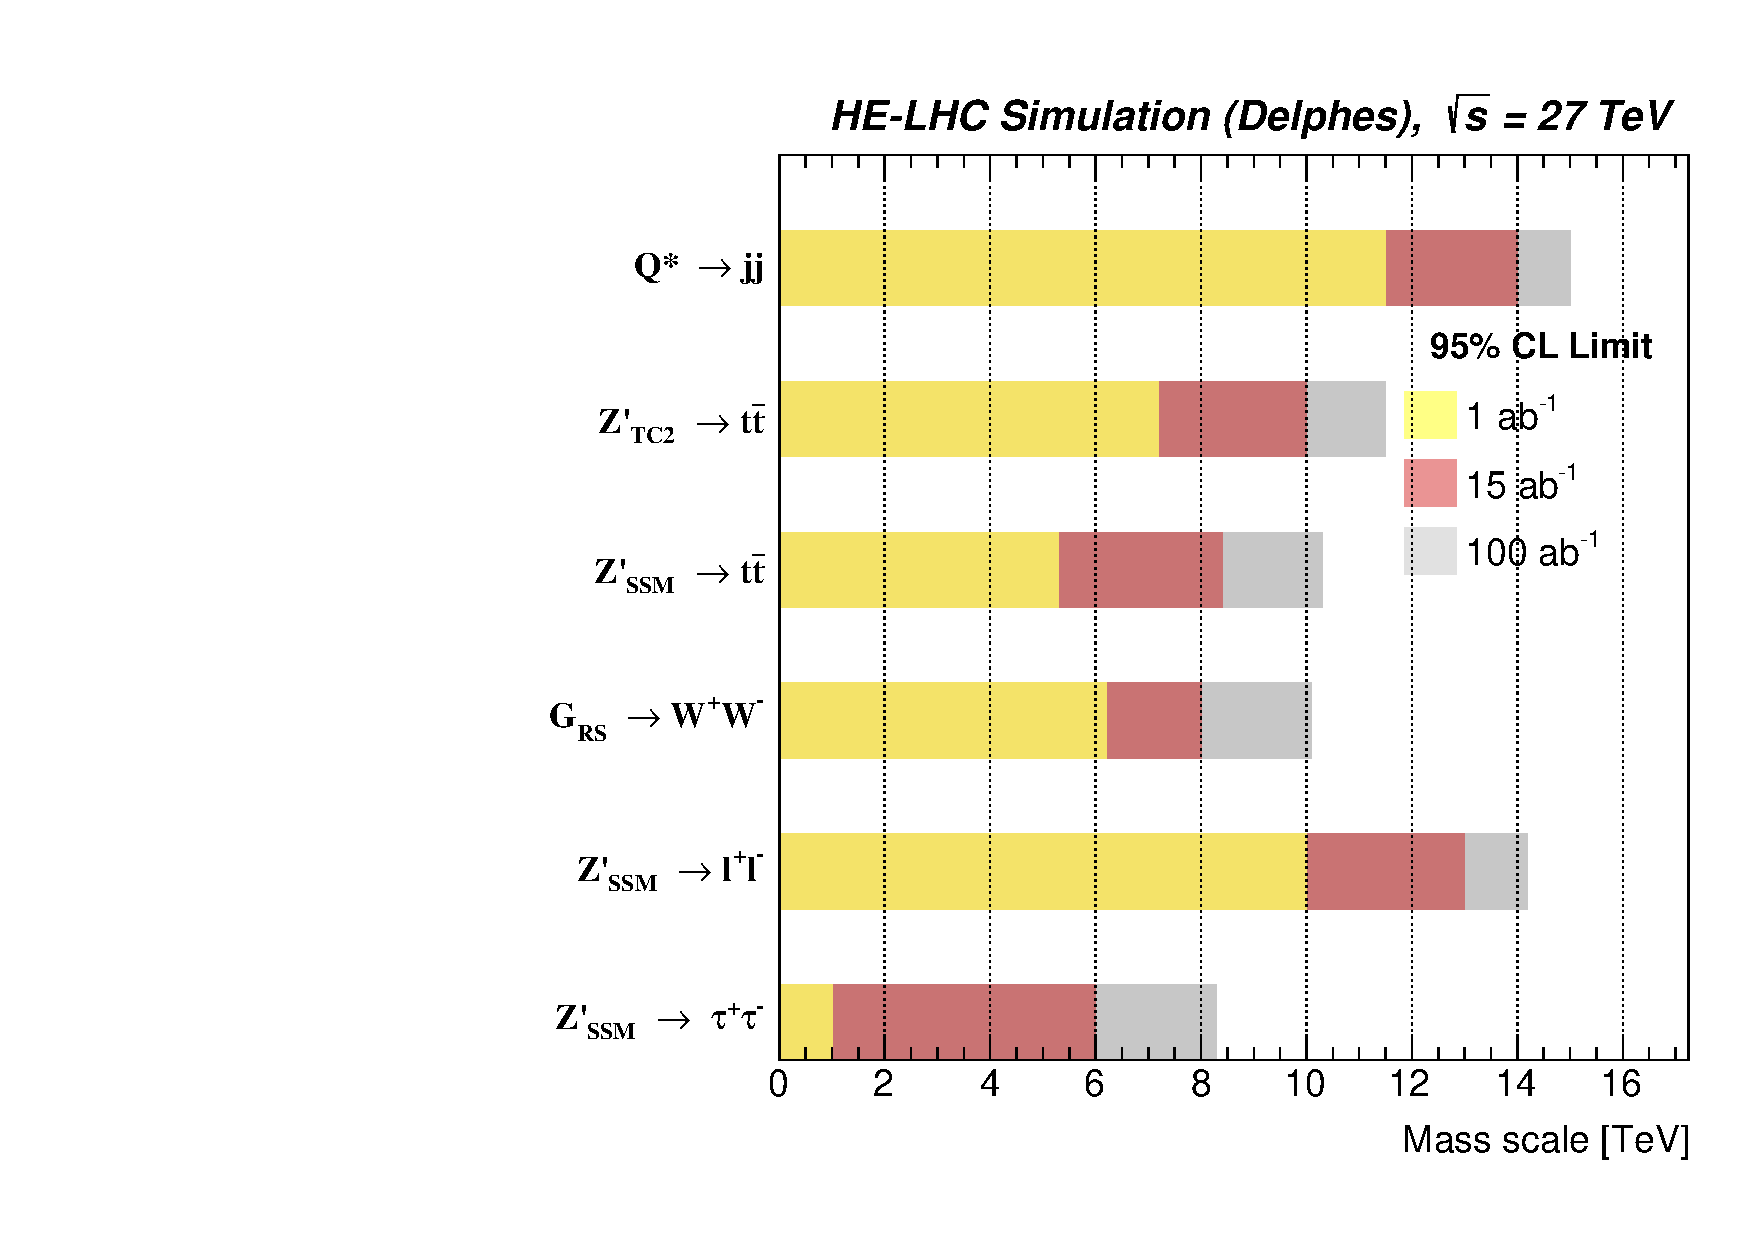
\includegraphics[width=0.49\columnwidth]{Fig/summaryLimit_onlyHELHC.pdf}
  \caption{Summary of a $5\sigma$ discovery reach (top) and 95\% CL limits (bottom) as a function of the resonance mass for different luminosity scenario of FCC-hh (left) and HE-LHC (right).}
  \label{figure:resonances100:summary}
\end{figure}


\acknowledgments

Thanks to...
The work of TGR was supported by the Department of Energy, Contract DE-AC02-76SF00515.
\paragraph{Note added.} This is also a good position for notes added
after the paper has been written.





% The bibliography will probably be heavily edited during typesetting.
% We'll parse it and, using the arxiv number or the journal data, will
% query inspire, trying to verify the data (this will probalby spot
% eventual typos) and retrive the document DOI and eventual errata.
% We however suggest to always provide author, title and journal data:
% in short all the informations that clearly identify a document.

\bibliographystyle{JHEP}
\bibliography{paper}

% Please avoid comments such as "For a review'', "For some examples",
% "and references therein" or move them in the text. In general,
% please leave only references in the bibliography and move all
% accessory text in footnotes.

% Also, please have only one work for each \bibitem.%appendix%appendix


\end{document}
